% =====================================================================================
\section{Results}
\label{sec:results}

This section reports the tests in the order of the method of Section~\ref{sec:method}, main method first. It starts with inputs that carry no instruction. First come the two published methods that we ran, with their instructions taken away (Section~\ref{sec:nodefpublished}). Next comes the recogniser \recog{} of Section~\ref{sec:audit}: what it recognises, on which tasks, and with which guarantee (Section~\ref{sec:recogniser}). Then come trained answers with its routes, against the published methods (Section~\ref{sec:nodeftrained}). After these come the certified switch \cert{} with instructions, routes from the example alone with instructions (Section~\ref{sec:exampleroutes}), the stress tests and variants of the zones, and the section ends with zones built from the inputs of a task (Section~\ref{sec:noinstruction}). Every test had its pass line written before the run (Section~\ref{sec:protocol}); where a choice or a line was changed after numbers had been seen, we say so.

\subsection{The published methods without their instructions}
\label{sec:nodefpublished}

This subsection starts the results with inputs that carry no instruction. It asks what the two published methods that we ran lose when the instruction of every task is taken away, and it counts the inputs that occur in two tasks, which set a limit to any method without instructions (Proposition~\ref{prop:noinstructionprice}). The rows of our own method in Table~\ref{tab:noinstpublished} use the recogniser \recog{} of Section~\ref{sec:audit}; it is tested in Section~\ref{sec:recogniser}, and the rows are explained in Section~\ref{sec:nodeftrained}.
Every test was written down in the plan of the repository before it was run, with the line by which it would be read (Section~\ref{sec:protocol}); the lines are repeated below, and so are the guesses that were wrong.

\paragraph{The published methods without their instructions.} We repeated the five-task run of Section~\ref{sec:five} for the two published methods that we ran, InfLoRA and GainLoRA (official code): the same five tasks, seed 42, model (T5-base) and 10 epochs per task, with one change.
The definition of every task was replaced by the empty string in every data file, for training and for testing, so that every input is the same fixed text followed by the instance.
Line fixed before the run, for each method against its own run with definitions: (1) if the score right after learning is below 60\% of the score with definitions, the method ``could not learn these tasks''; (2) if it learned, it ``holds its answers less well'' when forgetting rises by at least 5 points, or when the number of changed answers is at least twice as large and at least 60 of 400 higher.
Table~\ref{tab:noinstpublished} has the numbers.

\begin{table}[t]
  \caption{The five tasks of Section~\ref{sec:five}, T5-base, 10 epochs, seed 42, re-test (every reference answer is used). ``Definitions'': with the definition of every task in its inputs, or none (the empty string, in training and testing). Score right after learning: average score (Rouge-L) right after each task was learned. Final score: average final score. Forgetting: average forgetting. Answers changed: of the \AudPubCompared{} test inputs of the first four tasks, the answers that differ at the end from the answer right after their task was learned. Learned and AP are averages over the five tasks; FT and Changed are over the first four (the last task cannot be forgotten). The three rows of ours use plain adapters that are never blocked, with the routes of Section~\ref{sec:audit}; they were run without definitions only. The last row sends every input to its own task: the best that any route can give.}
  \label{tab:noinstpublished}
  \centering
  {\footnotesize\setlength{\tabcolsep}{3pt}\begin{tabular}{p{1.9in}lrrrr}
    \toprule
    Method & Definitions & \shortstack[r]{Score right\\after\\learning $\uparrow$} & \shortstack[r]{Final\\score $\uparrow$} & \shortstack[r]{Forgetting\\(points) $\downarrow$} & \shortstack[r]{Answers\\changed\\of \AudPubCompared{} $\downarrow$} \\
    \midrule
    InfLoRA & with & \AudPubInfloraDefLearned{} & \AudPubInfloraDefAP{} & \AudPubInfloraDefFT{} & \AudPubInfloraDefChanged{} \\
    InfLoRA & none & \AudPubInfloraNoDefLearned{} & \AudPubInfloraNoDefAP{} & \AudPubInfloraNoDefFT{} & \AudPubInfloraNoDefChanged{} \\
    GainLoRA & with & \AudPubGainloraDefLearned{} & \AudPubGainloraDefAP{} & \AudPubGainloraDefFT{} & \AudPubGainloraDefChanged{} \\
    GainLoRA & none & \AudPubGainloraNoDefLearned{} & \AudPubGainloraNoDefAP{} & \AudPubGainloraNoDefFT{} & \AudPubGainloraNoDefChanged{} \\
    \midrule
    \plain{} (all adapters on) & none & \AudOursAllLearned{} & \AudOursAllAP{} & \AudOursAllFT{} & \AudOursAllChanged{} \\
    \recog{} (ours) & none & \AudOursRidgeLearned{} & \AudOursRidgeAP{} & \AudOursRidgeFT{} & \AudOursRidgeChanged{} \\
    \handicap{}, $\nu = 2$ (ours) & none & \AudOursHandicapLearned{} & \AudOursHandicapAP{} & \AudOursHandicapFT{} & \AudOursHandicapChanged{} \\
    every input to its own task (ceiling) & none & \AudOursOwnLearned{} & \AudOursOwnAP{} & \AudOursOwnFT{} & \AudOursOwnChanged{} \\
    \bottomrule
\end{tabular}}

\end{table}

Both methods learned (the score right after learning without definitions is \AudPubInfloraNoDefLearned{} for InfLoRA and \AudPubGainloraNoDefLearned{} for GainLoRA, against \AudPubInfloraDefLearned{} and \AudPubGainloraDefLearned{} with definitions in this seed; the line was 60\%).
Both hold their answers less well, by the line fixed before: forgetting is \AudPubInfloraNoDefFT{} for InfLoRA (\AudPubInfloraDefFT{} with definitions) and \AudPubGainloraNoDefFT{} for GainLoRA (\AudPubGainloraDefFT{}); the final score falls from \AudPubInfloraDefAP{} to \AudPubInfloraNoDefAP{} and from \AudPubGainloraDefAP{} to \AudPubGainloraNoDefAP{}; and the changed answers rise from \AudPubInfloraDefChanged{} to \AudPubInfloraNoDefChanged{} and from \AudPubGainloraDefChanged{} to \AudPubGainloraNoDefChanged{} of \AudPubCompared{}.
(The line was set against the three-seed runs with definitions of Section~\ref{sec:five}; the table gives the same seed.)
Our guess for GainLoRA was 60 to 150 changed answers: \AudPubGainloraNoDefChanged{}.

Table~\ref{tab:conflictcount} counts what Proposition~\ref{prop:noinstructionprice} needs on the data used here: inputs that occur word for word in two tasks.
On both standard benchmarks, no input occurs in two tasks (\AudConfOneShared{} of \AudConfOneInputs{} inputs for the 15 SuperNI tasks, \AudConfTwoShared{} of \AudConfTwoInputs{} for the 15 Long Sequence tasks).
The count is a lower limit of the conflict: tasks can overlap without sharing a text word for word.
So the count alone shows only that no loss is forced by shared texts. That the loss of the two methods was not forced is shown by the recogniser of Section~\ref{sec:recogniser}, which gives all but \AudRouteFiveRidgeNotOwn{} of the \AudRouteFiveRidgeN{} test inputs of these five tasks to their own task without reading an instruction.

\begin{table}[t]
  \caption{Inputs that occur word for word in the data of two or more tasks. Rows are collections of tasks (training and test inputs of the benchmark tasks; the instances read from the task files for the fresh batches of the paragraph on fresh tasks in Section~\ref{sec:recogniser}). ``Also elsewhere'': inputs that occur in another task of the same collection; \%: their share of all inputs of the collection. A count, not a test.}
  \label{tab:conflictcount}
  \centering
  {\footnotesize\setlength{\tabcolsep}{3pt}\begin{tabular}{lrrrr}
    \toprule
    Collection & Tasks & Inputs & \shortstack[r]{Occur also\\in another\\task} & \shortstack[r]{Share,\\\%} \\
    \midrule
    SuperNI, 15 tasks & \AudConfOneTasks{} & \AudConfOneInputs{} & \AudConfOneShared{} & \AudConfOneShare{} \\
    Long Sequence, 15 tasks & \AudConfTwoTasks{} & \AudConfTwoInputs{} & \AudConfTwoShared{} & \AudConfTwoShare{} \\
    fresh batch 1 & \AudConfThreeTasks{} & \AudConfThreeInputs{} & \AudConfThreeShared{} & \AudConfThreeShare{} \\
    fresh batch 2 & \AudConfFourTasks{} & \AudConfFourInputs{} & \AudConfFourShared{} & \AudConfFourShare{} \\
    fresh batch 3 & \AudConfFiveTasks{} & \AudConfFiveInputs{} & \AudConfFiveShared{} & \AudConfFiveShare{} \\
    \bottomrule
\end{tabular}}

\end{table}

Caveats, written before the run: one seed, five tasks, a small model, a tenth of the published number of epochs. Only these two methods were run: this is a first look at two methods in a reduced setting, and says nothing about other methods. Two more seeds were run afterwards (Table~\ref{tab:noinstseeds} in Section~\ref{sec:nodeftrained}). Over the three seeds InfLoRA changes \AudSeedsInfloraChanged{} and GainLoRA \AudSeedsGainloraChanged{} of \AudSeedsCompared{} answers without definitions, against \FiveInfChanged{} and \FiveGainChanged{} with them (Section~\ref{sec:five}), and their forgetting is \AudSeedsInfloraFT{} and \AudSeedsGainloraFT{} points against \FiveInfFT{} and \FiveGainFT{}: the reading is the same in every seed. With their published number of epochs the two methods learn the five tasks and then lose far more (Section~\ref{sec:nodeftrained}, Table~\ref{tab:noinstfull}).

\medskip
\noindent The per-task scores of this run follow.

\begin{table}[t]
  \caption{Per-task scores of the five-task run of Table~\ref{tab:noinstpublished} (re-test): score right after the task was learned $\to$ score at the end, Rouge-L. Columns: the two published methods with the definitions in the inputs and with none, and our \recog{} with none (plain adapters). Rows: the five tasks in their order. The last task cannot be forgotten.}
  \label{tab:noinstpertask}
  \centering
  {\footnotesize\setlength{\tabcolsep}{2pt}\begin{tabular}{lrrrrr}
    \toprule
    & \multicolumn{5}{c}{\shortstack{Score right after learning\\$\to$ at the end $\uparrow$}} \\
    \cmidrule(l){2-6}
    & \multicolumn{2}{c}{InfLoRA} & \multicolumn{2}{c}{GainLoRA} & ours (L) \\
    \cmidrule(lr){2-3}\cmidrule(lr){4-5}\cmidrule(l){6-6}
    Task & with & none & with & none & none \\
    \midrule
    relation extr. & \AudPubInfloraDefPtLearnedRelation{}\,$\to$\,\AudPubInfloraDefPtFinalRelation{} & \AudPubInfloraNoDefPtLearnedRelation{}\,$\to$\,\AudPubInfloraNoDefPtFinalRelation{} & \AudPubGainloraDefPtLearnedRelation{}\,$\to$\,\AudPubGainloraDefPtFinalRelation{} & \AudPubGainloraNoDefPtLearnedRelation{}\,$\to$\,\AudPubGainloraNoDefPtFinalRelation{} & \AudOursPtLearnedRelation{}\,$\to$\,\AudOursPtFinalRelation{} \\
    sst2 & \AudPubInfloraDefPtLearnedSst{}\,$\to$\,\AudPubInfloraDefPtFinalSst{} & \AudPubInfloraNoDefPtLearnedSst{}\,$\to$\,\AudPubInfloraNoDefPtFinalSst{} & \AudPubGainloraDefPtLearnedSst{}\,$\to$\,\AudPubGainloraDefPtFinalSst{} & \AudPubGainloraNoDefPtLearnedSst{}\,$\to$\,\AudPubGainloraNoDefPtFinalSst{} & \AudOursPtLearnedSst{}\,$\to$\,\AudOursPtFinalSst{} \\
    glucose & \AudPubInfloraDefPtLearnedGlucose{}\,$\to$\,\AudPubInfloraDefPtFinalGlucose{} & \AudPubInfloraNoDefPtLearnedGlucose{}\,$\to$\,\AudPubInfloraNoDefPtFinalGlucose{} & \AudPubGainloraDefPtLearnedGlucose{}\,$\to$\,\AudPubGainloraDefPtFinalGlucose{} & \AudPubGainloraNoDefPtLearnedGlucose{}\,$\to$\,\AudPubGainloraNoDefPtFinalGlucose{} & \AudOursPtLearnedGlucose{}\,$\to$\,\AudOursPtFinalGlucose{} \\
    sentiment140 & \AudPubInfloraDefPtLearnedSentiment{}\,$\to$\,\AudPubInfloraDefPtFinalSentiment{} & \AudPubInfloraNoDefPtLearnedSentiment{}\,$\to$\,\AudPubInfloraNoDefPtFinalSentiment{} & \AudPubGainloraDefPtLearnedSentiment{}\,$\to$\,\AudPubGainloraDefPtFinalSentiment{} & \AudPubGainloraNoDefPtLearnedSentiment{}\,$\to$\,\AudPubGainloraNoDefPtFinalSentiment{} & \AudOursPtLearnedSentiment{}\,$\to$\,\AudOursPtFinalSentiment{} \\
    emotion & \AudPubInfloraDefPtLearnedEmotion{}\,$\to$\,\AudPubInfloraDefPtFinalEmotion{} & \AudPubInfloraNoDefPtLearnedEmotion{}\,$\to$\,\AudPubInfloraNoDefPtFinalEmotion{} & \AudPubGainloraDefPtLearnedEmotion{}\,$\to$\,\AudPubGainloraDefPtFinalEmotion{} & \AudPubGainloraNoDefPtLearnedEmotion{}\,$\to$\,\AudPubGainloraNoDefPtFinalEmotion{} & \AudOursPtLearnedEmotion{}\,$\to$\,\AudOursPtFinalEmotion{} \\
    \bottomrule
\end{tabular}}

\end{table}


\subsection{Recognising the task without an instruction}
\label{sec:recogniser}

This subsection tests the recogniser \recog{} and its variant \handicap{}, which has a bound in advance (Section~\ref{sec:audit}); both read no instruction and block no task. The tests are: a feature that separates the tasks; rules that block nothing and the handicap; four zone shapes (run earlier); fresh tasks; the second benchmark and many tasks. The rule that builds zones from the inputs of a task (Section~\ref{sec:bound}) was tested first; that test, reported in Section~\ref{sec:noinstruction} at the end of this section, left a better frozen feature as the open question.
Every test was written down in the plan of the repository before it was run, with the line by which it would be read (Section~\ref{sec:protocol}); the lines are repeated below, and so are the guesses that were wrong. The exceptions are the corrected form of \handicap{} and its setting, which were chosen after numbers had been seen and are marked as such.

\paragraph{The feature.} The zone rule of Section~\ref{sec:noinstruction} (zones built from the inputs of a task; the ratio score, level 0.05, the oldest zone wins) was run with a third frozen feature: the mean of the last-layer states of the frozen T5-base encoder, without any adapter, over the tokens of the instance.
Its first test, with two other features, was run before the recogniser existed and is reported in Section~\ref{sec:noinstruction}.
Development data: the 15 SuperNI tasks of order 1, at most 400 training inputs per task, official test inputs.
Line fixed before the run: ``works'' if on average at least 90\% of the test inputs reach their own task and at most 10\% are blocked.
The guess written before was 20 to 35\% blocked.
Table~\ref{tab:recogniserfeatures} (top) shows \AudZoneFrozenTBlocked{}\% blocked and \AudZoneFrozenTOwn{}\% given to their own task, against \AudZoneSentenceBlocked{}\% and \AudZoneSentenceOwn{}\% for the sentence encoder and \AudZoneWordVecBlocked{}\% and \AudZoneWordVecOwn{}\% for the word vectors; the changed routes are \AudZoneFrozenTChanged{}\%, within the claim.
By the line the verdict is ``partial'': just below 90\% own task and just above 10\% blocked.
The guess was wrong in the good direction.
A likely reason: a sentence encoder is built to keep what a text is about and to discard how it is written, and how an input is written is most of what separates tasks.
The middle of the table shows the same lesson for a joint recogniser (Section~\ref{sec:audit}) on sentence-encoder features: adding 16 simple numbers that describe the shape of the text (length, capitals, digits, punctuation, line breaks, @, \# and web addresses) raises the share given to the own task at the end from \AudRecLrMiniEndSuperni{}\% to \AudRecLrShapeEndSuperni{}\% on the SuperNI tasks and from \AudRecLrMiniEndLong{}\% to \AudRecLrShapeEndLong{}\% on the Long Sequence tasks; character n-grams give \AudRecLrCharEndSuperni{}\% and \AudRecLrCharEndLong{}\%.

\begin{table}[t]
  \caption{Features, development data (the benchmark tasks were used to choose among the variants). Top: the zone rule of Section~\ref{sec:noinstruction} with three frozen features on the 15 SuperNI tasks; means over the tasks, in \%: test inputs inside their own zone; blocked by an older zone when their task arrives; given to their own task after the last task; whose route changed after their task arrived. Middle: a joint recogniser over all tasks, fitted by logistic regression on stored fit features or by Eq.~\eqref{eq:recogniser} on random cosine features, on the sentence encoder with or without the shape numbers or character n-grams, for the 15 SuperNI and the 15 Long Sequence tasks; the last pair of columns is $(H{+}1)/(m{+}1)$, where $H$ of the $m$ held-out inputs of a task changed route (Proposition~\ref{prop:audit}), the line against which the change was read. Bottom: the audit of Proposition~\ref{prop:audit} for the variant that was chosen (logistic regression with shape numbers): the estimate $H/m$ and the 95\% bound, averaged over the tasks.}
  \label{tab:recogniserfeatures}
  \centering
  {\footnotesize\setlength{\tabcolsep}{3pt}\begin{tabular}{lrrrr}
    \toprule
    Feature & \shortstack[r]{Inside own\\zone, \%} & \shortstack[r]{Blocked,\\\% $\downarrow$} & \shortstack[r]{Sent to\\own task\\at the end,\\\% $\uparrow$} & \shortstack[r]{Route\\changed,\\\% $\downarrow$} \\
    \midrule
    word vectors & \AudZoneWordVecInside{} & \AudZoneWordVecBlocked{} & \AudZoneWordVecOwn{} & \AudZoneWordVecChanged{} \\
    sentence encoder & \AudZoneSentenceInside{} & \AudZoneSentenceBlocked{} & \AudZoneSentenceOwn{} & \AudZoneSentenceChanged{} \\
    frozen T5-base states & \AudZoneFrozenTInside{} & \AudZoneFrozenTBlocked{} & \AudZoneFrozenTOwn{} & \AudZoneFrozenTChanged{} \\
    \bottomrule
\end{tabular}}
\par\medskip
{\footnotesize\setlength{\tabcolsep}{1.8pt}\begin{tabular}{lrrrrrr}
    \toprule
    & \multicolumn{2}{c}{\shortstack{Sent to own task\\at the end, \% $\uparrow$}} & \multicolumn{2}{c}{\shortstack{Route changed,\\\% $\downarrow$}} & \multicolumn{2}{c}{\shortstack{Audit\\$(H{+}1)/(m{+}1)$, \%}} \\
    \cmidrule(lr){2-3}\cmidrule(lr){4-5}\cmidrule(l){6-7}
    Recogniser, feature & SuperNI & Long & SuperNI & Long & SuperNI & Long \\
    \midrule
    logistic reg., sentence enc., $C=$\AudRecLrMiniParam{} & \AudRecLrMiniEndSuperni{} & \AudRecLrMiniEndLong{} & \AudRecLrMiniChangedSuperni{} & \AudRecLrMiniChangedLong{} & \AudRecLrMiniAuditLineSuperni{} & \AudRecLrMiniAuditLineLong{} \\
    \textbf{\quad + shape numbers, $C=$\AudRecLrShapeParam{}} & \textbf{\AudRecLrShapeEndSuperni{}} & \textbf{\AudRecLrShapeEndLong{}} & \textbf{\AudRecLrShapeChangedSuperni{}} & \textbf{\AudRecLrShapeChangedLong{}} & \textbf{\AudRecLrShapeAuditLineSuperni{}} & \textbf{\AudRecLrShapeAuditLineLong{}} \\
    \quad + character n-grams, $C=$\AudRecLrCharParam{} & \AudRecLrCharEndSuperni{} & \AudRecLrCharEndLong{} & \AudRecLrCharChangedSuperni{} & \AudRecLrCharChangedLong{} & \AudRecLrCharAuditLineSuperni{} & \AudRecLrCharAuditLineLong{} \\
    cosine features, sentence enc., $\lambda=$\AudRecCosMiniParam{} & \AudRecCosMiniEndSuperni{} & \AudRecCosMiniEndLong{} & \AudRecCosMiniChangedSuperni{} & \AudRecCosMiniChangedLong{} & \AudRecCosMiniAuditLineSuperni{} & \AudRecCosMiniAuditLineLong{} \\
    \quad + shape numbers, $\lambda=$\AudRecCosShapeParam{} & \AudRecCosShapeEndSuperni{} & \AudRecCosShapeEndLong{} & \AudRecCosShapeChangedSuperni{} & \AudRecCosShapeChangedLong{} & \AudRecCosShapeAuditLineSuperni{} & \AudRecCosShapeAuditLineLong{} \\
    \bottomrule
\end{tabular}}
\par\medskip
{\footnotesize\setlength{\tabcolsep}{3pt}\begin{tabular}{lrrrr}
    \toprule
    & \multicolumn{2}{c}{Audit $H/m$, \%} & \multicolumn{2}{c}{95\% bound, \%} \\
    \cmidrule(lr){2-3}\cmidrule(l){4-5}
    Chosen variant & SuperNI & Long & SuperNI & Long \\
    \midrule
    logistic reg. + shape numbers, $C=$\AudRecLrShapeParam{} & \AudRecChosenAuditEstSuperni{} & \AudRecChosenAuditEstLong{} & \AudRecChosenAuditBoundSuperni{} & \AudRecChosenAuditBoundLong{} \\
    \bottomrule
\end{tabular}}

\end{table}

\paragraph{Rules that block nothing.} Development data: the 15 SuperNI tasks, at most 400 training inputs per task, 200 of them held out (half for the tasks with fewer than 400), and the official test inputs.
Table~\ref{tab:recogniserdev} gives the rules on the frozen T5-base states, standardised with the statistics of 2{,}000 instances of other SuperNI tasks (the pool of Section~\ref{sec:protocol}, not $\mathcal{B}$).
Rule written before the run: among the variants with at most 3\% changed routes, take the highest share of test inputs given to their own task after the last task; ties go to the ridge form, which stores no input.
The rule chose \recog{} with the smallest of three penalties (``ridge $1\times$'': in the code a penalty equal to the feature dimension, 768, on sums in which every task has a total weight of 200; in Eq.~\eqref{eq:recogniser} this is $\varepsilon = 768/200 = 3.84$), tied with the logistic regression.
It gives \AudDevLLamOneArrive{}\% of the test inputs to their own task right after their task arrives and \AudDevLLamOneEnd{}\% after the last task, and \AudDevLLamOneChanged{}\% of the routes change.
Our guess before the run was 95 to 99\% on the 15 tasks; it held. We also guessed 1 to 3\% changed routes; it was \AudDevLLamOneChanged{}\%.
The weights after all 15 tasks are the same for every order of arrival, up to floating-point rounding (checked with the order reversed); on the second official order and on five random orders (Table~\ref{tab:recogniserorders}) the changed routes run from \AudOrdRandTwoLChanged{}\% to \AudOrdTwoLChanged{}\%.
The audit of Proposition~\ref{prop:audit} says \AudDevLLamOneAuditEst{}\% for the average task, with a 95\% bound of \AudDevLLamOneAuditBound{}\%, next to the \AudDevLLamOneChanged{}\% that changed on the test inputs.

\begin{table}[t]
  \caption{Rules that block nothing, development data: the 15 SuperNI tasks of order 1, frozen T5-base states, official test inputs; means over the tasks, in \%. ``Own task'': test inputs given to their own task right after it arrived and after the last task. ``Route changed'': test inputs whose route after the last task differs from the route when their task arrived. Audit $H/m$ and 95\% bound: Proposition~\ref{prop:audit}, from the held-out inputs. Bound in advance: Theorem~\ref{thm:handicap} for \handicap{}, averaged over the tasks; for the zone rule, the line described in the paragraph on zones below (not a theorem of this paper). $C$: the inverse penalty of the logistic regression. Ridge $1\times$, $10\times$, $100\times$: the penalty of Eq.~\eqref{eq:recogniser} in multiples of the smallest. $r$: a new zone may hold at most $r - 1$ held-out inputs of an older task. Bold: the variants used later. The last three rows are the first form of \handicap{}, without the floor at zero in Eq.~\eqref{eq:handicap}. The rows were compared on these tasks, so these are development numbers.}
  \label{tab:recogniserdev}
  \centering
  {\scriptsize\setlength{\tabcolsep}{2.5pt}\begin{tabular}{p{1.6in}rrrrrr}
    \toprule
    Rule & \shortstack[r]{Sent to\\own task\\at arrival,\\\% $\uparrow$} & \shortstack[r]{Sent to\\own task\\at the end,\\\% $\uparrow$} & \shortstack[r]{Route\\changed,\\\% $\downarrow$} & \shortstack[r]{Audit\\$H/m$, \%} & \shortstack[r]{95\% bound,\\\%} & \shortstack[r]{Bound in\\advance, \%} \\
    \midrule
    \recog{} with logistic regression ($C = 1$) & \AudDevJCOneArrive{} & \AudDevJCOneEnd{} & \AudDevJCOneChanged{} & \AudDevJCOneAuditEst{} & \AudDevJCOneAuditBound{} & -- \\
    \textbf{\recog{}, ridge $1\times$} & \textbf{\AudDevLLamOneArrive{}} & \textbf{\AudDevLLamOneEnd{}} & \textbf{\AudDevLLamOneChanged{}} & \textbf{\AudDevLLamOneAuditEst{}} & \textbf{\AudDevLLamOneAuditBound{}} & \textbf{--} \\
    \recog{}, ridge $10\times$ & \AudDevLLamTenArrive{} & \AudDevLLamTenEnd{} & \AudDevLLamTenChanged{} & \AudDevLLamTenAuditEst{} & \AudDevLLamTenAuditBound{} & -- \\
    \recog{}, ridge $100\times$ & \AudDevLLamHundredArrive{} & \AudDevLLamHundredEnd{} & \AudDevLLamHundredChanged{} & \AudDevLLamHundredAuditEst{} & \AudDevLLamHundredAuditBound{} & -- \\
    zones, newest wins, $r = 1$ & \AudDevClaimsROneArrive{} & \AudDevClaimsROneEnd{} & \AudDevClaimsROneChanged{} & -- & -- & \AudDevClaimsROneBound{} \\
    \handicap{}, $\nu = 0$ & \AudDevHPrimeTZeroArrive{} & \AudDevHPrimeTZeroEnd{} & \AudDevHPrimeTZeroChanged{} & -- & -- & \AudDevHPrimeTZeroBound{} \\
    \handicap{}, $\nu = 1$ & \AudDevHPrimeTOneArrive{} & \AudDevHPrimeTOneEnd{} & \AudDevHPrimeTOneChanged{} & -- & -- & \AudDevHPrimeTOneBound{} \\
    \textbf{\handicap{}, $\nu = 2$} & \textbf{\AudDevHPrimeTTwoArrive{}} & \textbf{\AudDevHPrimeTTwoEnd{}} & \textbf{\AudDevHPrimeTTwoChanged{}} & \textbf{--} & \textbf{--} & \textbf{\AudDevHPrimeTTwoBound{}} \\
    \handicap{}, $\nu = 5$ & \AudDevHPrimeTFiveArrive{} & \AudDevHPrimeTFiveEnd{} & \AudDevHPrimeTFiveChanged{} & -- & -- & \AudDevHPrimeTFiveBound{} \\
    \handicap{} without protection ($\nu = \infty$) & \AudDevHPrimeTNoneArrive{} & \AudDevHPrimeTNoneEnd{} & \AudDevHPrimeTNoneChanged{} & -- & -- & -- \\
    \midrule
    \handicap{} without the floor (first form), $\nu = 0$ & \AudDevHTZeroArrive{} & \AudDevHTZeroEnd{} & \AudDevHTZeroChanged{} & -- & -- & \AudDevHTZeroBound{} \\
    \handicap{} without the floor (first form), $\nu = 1$ & \AudDevHTOneArrive{} & \AudDevHTOneEnd{} & \AudDevHTOneChanged{} & -- & -- & \AudDevHTOneBound{} \\
    \handicap{} without the floor (first form), $\nu = 2$ & \AudDevHTTwoArrive{} & \AudDevHTTwoEnd{} & \AudDevHTTwoChanged{} & -- & -- & \AudDevHTTwoBound{} \\
    \bottomrule
\end{tabular}}

\end{table}

\begin{table}[t]
  \caption{\recog{} (ridge $1\times$) and \handicap{} ($\nu = 2$) on other orders of the same 15 SuperNI tasks, development data: the second official order and five random orders. Columns as in Table~\ref{tab:recogniserdev}; $(H{+}1)/(m{+}1)$ is the line against which the changed routes were read, and the 95\% bound is the audit's.}
  \label{tab:recogniserorders}
  \centering
  {\footnotesize\setlength{\tabcolsep}{3pt}\begin{tabular}{lrrrrrrr}
    \toprule
    & \multicolumn{5}{c}{\recog{}} & \multicolumn{2}{c}{\handicap{}, $\nu = 2$} \\
    \cmidrule(lr){2-6}\cmidrule(l){7-8}
    Order & \shortstack[r]{Sent to\\own task\\at arrival,\\\% $\uparrow$} & \shortstack[r]{Sent to\\own task\\at the end,\\\% $\uparrow$} & \shortstack[r]{Route\\changed,\\\% $\downarrow$} & \shortstack[r]{$(c{+}1)/$\\$(m{+}1)$, \%} & \shortstack[r]{95\% bound,\\\%} & \shortstack[r]{Sent to\\own task\\at the end,\\\% $\uparrow$} & \shortstack[r]{Route\\changed,\\\% $\downarrow$} \\
    \midrule
    order 1 & \AudOrdOneLArrive{} & \AudOrdOneLEnd{} & \AudOrdOneLChanged{} & \AudOrdOneLAuditLine{} & \AudOrdOneLAuditBound{} & \AudOrdOneHEnd{} & \AudOrdOneHChanged{} \\
    order 2 & \AudOrdTwoLArrive{} & \AudOrdTwoLEnd{} & \AudOrdTwoLChanged{} & \AudOrdTwoLAuditLine{} & \AudOrdTwoLAuditBound{} & \AudOrdTwoHEnd{} & \AudOrdTwoHChanged{} \\
    random 0 & \AudOrdRandZeroLArrive{} & \AudOrdRandZeroLEnd{} & \AudOrdRandZeroLChanged{} & \AudOrdRandZeroLAuditLine{} & \AudOrdRandZeroLAuditBound{} & \AudOrdRandZeroHEnd{} & \AudOrdRandZeroHChanged{} \\
    random 1 & \AudOrdRandOneLArrive{} & \AudOrdRandOneLEnd{} & \AudOrdRandOneLChanged{} & \AudOrdRandOneLAuditLine{} & \AudOrdRandOneLAuditBound{} & \AudOrdRandOneHEnd{} & \AudOrdRandOneHChanged{} \\
    random 2 & \AudOrdRandTwoLArrive{} & \AudOrdRandTwoLEnd{} & \AudOrdRandTwoLChanged{} & \AudOrdRandTwoLAuditLine{} & \AudOrdRandTwoLAuditBound{} & \AudOrdRandTwoHEnd{} & \AudOrdRandTwoHChanged{} \\
    random 3 & \AudOrdRandThreeLArrive{} & \AudOrdRandThreeLEnd{} & \AudOrdRandThreeLChanged{} & \AudOrdRandThreeLAuditLine{} & \AudOrdRandThreeLAuditBound{} & \AudOrdRandThreeHEnd{} & \AudOrdRandThreeHChanged{} \\
    random 4 & \AudOrdRandFourLArrive{} & \AudOrdRandFourLEnd{} & \AudOrdRandFourLChanged{} & \AudOrdRandFourLAuditLine{} & \AudOrdRandFourLAuditBound{} & \AudOrdRandFourHEnd{} & \AudOrdRandFourHChanged{} \\
    \bottomrule
\end{tabular}}

\end{table}

Where it is weak: the tweet task (sentiment140) falls from \AudPtFourteenArrive{}\% to \AudPtFourteenEnd{}\% when the emotion task arrives (\AudPtFourteenC{} of its \AudPtFourteenM{} held-out inputs change route; audit \AudPtFourteenAuditEst{}\%, bound \AudPtFourteenBound{}\%; \AudPtFourteenChanged{}\% of its test inputs did change); the dialogue task (multi-woz) ends at \AudPtSevenEnd{}\%.
All other tasks end at 99 to 100\% (Table~\ref{tab:recogniserpertask}, at the end of this subsection).

\paragraph{\handicap{}, and a flaw in its first form.} \handicap{} (Eq.~\eqref{eq:handicap}) puts a bound known in advance on the same joint recogniser.
As first written, the threshold $\eta_k$ had no floor at zero.
When no held-out input of an older task lies near the newcomer, the threshold is then negative, and the newcomer takes inputs that even the joint recogniser gives to an older task.
For $\nu = 1$ and $2$ the first form changed more routes than no protection at all: \AudDevHTOneChanged{}\% and \AudDevHTTwoChanged{}\%, against \AudDevHPrimeTNoneChanged{}\% without protection. Our guess for the first form with $\nu = 0$ had been 97 to 99\% of the test inputs at their own task; it gave \AudDevHTZeroEnd{}\%.
The floor at zero is the correction.
It was made after seeing these numbers, on the same 15 tasks, so the numbers of the corrected rule are development numbers and no more; the proof is unchanged.
With the floor, \handicap{} gives at the end \AudDevHPrimeTZeroEnd{}\%, \AudDevHPrimeTOneEnd{}\% and \AudDevHPrimeTTwoEnd{}\% of the test inputs to their own task for $\nu = 0, 1, 2$, and changes \AudDevHPrimeTZeroChanged{}\%, \AudDevHPrimeTOneChanged{}\% and \AudDevHPrimeTTwoChanged{}\% of the routes; without protection the figures are \AudDevHPrimeTNoneEnd{}\% and \AudDevHPrimeTNoneChanged{}\%.
After seeing these numbers we chose $\nu = 2$, the smallest value within 0.2 points of the best at the end (the best was $\nu = 5$: \AudDevHPrimeTFiveEnd{}\%, with a bound of \AudDevHPrimeTFiveBound{}\%).
With $\nu = 0$ one task pays: quoref takes only about a third of its own inputs, because one held-out input of the news task sets the threshold (Remark~\ref{rem:auditlimits}(ii)).
For $\nu = 2$ the bound in advance, averaged over the tasks, is \AudDevHPrimeTTwoBound{}\%; what was measured is \AudDevHPrimeTTwoChanged{}\%.
The bound is loose, because most later tasks take nothing from most older ones, which it cannot know.

\paragraph{Zones can do it too, with the right feature.} In an earlier step, before the joint recogniser was chosen, four zone shapes were compared on the sentence encoder, under one rule: the newest zone wins, and no held-out input of an older task may lie inside a new zone, so no task is blocked.
Table~\ref{tab:shapesgrid} gives the share of test inputs that reach their own task at the end on the 15 SuperNI tasks (development data; the Long Sequence part of the grid was not computed).
The shape matters less than the feature: with the shape numbers three of the four shapes reach \AudShapeOvrShapeEnd{}\% to \AudShapePairShapeEnd{}\%, the balls fall to \AudShapePairKnnShapeEnd{}\%, and without the numbers the same three are at \AudShapeOvrMiniEnd{}\% to \AudShapePairMiniEnd{}\%.
The rule written before the grid chose one boundary per older task with the shape numbers (weight \AudShapePairShapeWeight{}): \AudShapePairShapeEnd{}\% at the end, \AudShapePairShapeChanged{}\% of the routes changed, against a line of \AudShapePairShapeBound{}\% on average. For this zone rule the line is the share of a task's test inputs outside its own zone when the task arrives, plus $r/(m+1)$ for every later task, where a new zone may hold at most $r - 1$ held-out inputs of an older task. It follows from the same rank argument as Theorem~\ref{thm:handicap}, but we use it as a line fixed in advance and do not state it as a theorem of this paper.
No guess was written down for the shapes.

\begin{table}[t]
  \caption{Four shapes of zone, development data: the 15 SuperNI tasks, the sentence encoder alone or with the 16 shape numbers (the weight of the numbers is the best of those tried). Rows: one flat boundary against everything older, one flat boundary per older task, balls around the task's inputs, boundaries curved by random cosine features. Means over the tasks, in \%: test inputs given to their own task after the last task; test inputs whose route changed. Bold: the variant chosen by the rule written before the grid.}
  \label{tab:shapesgrid}
  \centering
  {\footnotesize\setlength{\tabcolsep}{3pt}\begin{tabular}{lrrrrr}
    \toprule
    & \multicolumn{2}{c}{Sentence encoder} & \multicolumn{3}{c}{+ shape numbers} \\
    \cmidrule(lr){2-3}\cmidrule(l){4-6}
    Boundary & \shortstack[r]{Sent to\\own task\\at the end,\\\% $\uparrow$} & \shortstack[r]{Route\\changed,\\\% $\downarrow$} & \shortstack[r]{Sent to\\own task\\at the end,\\\% $\uparrow$} & \shortstack[r]{Route\\changed,\\\% $\downarrow$} & weight \\
    \midrule
    one boundary against everything & \AudShapeOvrMiniEnd{} & \AudShapeOvrMiniChanged{} & \AudShapeOvrShapeEnd{} & \AudShapeOvrShapeChanged{} & \AudShapeOvrShapeWeight{} \\
    one boundary per older task & \AudShapePairMiniEnd{} & \AudShapePairMiniChanged{} & \textbf{\AudShapePairShapeEnd{}} & \textbf{\AudShapePairShapeChanged{}} & \textbf{\AudShapePairShapeWeight{}} \\
    balls around the task's inputs & \AudShapePairKnnMiniEnd{} & \AudShapePairKnnMiniChanged{} & \AudShapePairKnnShapeEnd{} & \AudShapePairKnnShapeChanged{} & \AudShapePairKnnShapeWeight{} \\
    curved boundaries & \AudShapePairRffMiniEnd{} & \AudShapePairRffMiniChanged{} & \AudShapePairRffShapeEnd{} & \AudShapePairRffShapeChanged{} & \AudShapePairRffShapeWeight{} \\
    \bottomrule
\end{tabular}}

\end{table}

\paragraph{Fresh tasks.} Each rule of this paragraph was chosen on the 15 benchmark tasks and then read once on a batch of 30 fresh tasks that no earlier test had used (drawn at random from a collection of real tasks, instances only; at least 1{,}000 instances each, the last 200 as test inputs, and training and held-out inputs from a random part of the first 800).
Lines fixed before: the rule ``works'' if on average at least 85\% of the test inputs go to their own task, both right after their task arrives and after the last task; it ``does not'' below 70\%; between the two it is ``partial''. For the rule in which the oldest zone wins, the line also asked for at most 15\% blocked inputs, and read ``does not'' above 30\%.
For rules with a guarantee, the guarantee is ``met'' if the average changed share is at most the average bound (or, for the audit, the average $(H{+}1)/(m{+}1)$) plus two standard errors.
Table~\ref{tab:recogniserfresh} gives the rows that exist.
On the first batch the two zone rules on the sentence encoder did not work: the oldest zone wins gives \AudShapeFreshFirstOldestEnd{}\% to the own task at the end with \AudShapeFreshFirstOldestBlocked{}\% blocked (``\AudShapeFreshFirstOldestUse{}''), the newest zone wins \AudShapeFreshFirstNewestEnd{}\% (``\AudShapeFreshFirstNewestUse{}'').
On the second batch the zone rule with one boundary per older task and the shape numbers reaches \AudShapeFreshSecondEnd{}\% at the end and \AudShapeFreshSecondArrive{}\% at arrival, with \AudShapeFreshSecondChanged{}\% of the routes changed against its line of \AudShapeFreshSecondBound{}\% (see the paragraph on zones above): ``\AudShapeFreshSecondUse{}'', guarantee ``\AudShapeFreshSecondGuarantee{}''.
On the third batch the joint recogniser (logistic regression, sentence encoder and shape numbers) reaches \AudFreshThirdArrive{}\% and \AudFreshThirdEnd{}\%, with \AudFreshThirdChanged{}\% of the routes changed, audit \AudFreshThirdAuditEst{}\% and a 95\% bound of \AudFreshThirdAuditBound{}\% (line \AudFreshThirdAuditLine{}\%): ``\AudFreshThirdUse{}'', audit ``\AudFreshThirdCert{}''.
On the fourth batch \recog{} on the frozen model's states, the rule that is used for trained answers in Section~\ref{sec:nodeftrained}, reaches \AudFreshFourthLArrive{}\% at arrival and \AudFreshFourthLEnd{}\% at the end, with \AudFreshFourthLChanged{}\% of the routes changed, audit \AudFreshFourthAuditEst{}\% and a 95\% bound of \AudFreshFourthAuditBound{}\% (line \AudFreshFourthLAuditLine{}\%): ``\AudFreshFourthUse{}'', audit ``\AudFreshFourthCert{}''.
Our guess had been 80 to 90\%.
\handicap{} ($\nu = 2$), reported next to it on the same batch by a line fixed before (within 2 points of \recog{} at the end), reaches \AudFreshFourthHEnd{}\% and changes \AudFreshFourthHChanged{}\% of the routes.
The batches differ, so the rows do not compare the rules.

\begin{table}[t]
  \caption{Fresh tasks: each rule was chosen on the benchmark tasks and read once on a batch of 30 tasks that nothing had used. Rows: the rule and the batch. Columns, means over the 30 tasks, in \%: test inputs given to their own task right after their task arrived and after the last task; routes changed; audit $H/m$ and 95\% bound where the rule has an audit. Verdict: use / guarantee, by the lines in the text (works: at least 85\% own task at arrival and at the end; does not: below 70\%; else partial). The last column is the number of tasks below 70\% own task.}
  \label{tab:recogniserfresh}
  \centering
  {\scriptsize\setlength{\tabcolsep}{2pt}\begin{tabular}{p{0.95in}rrrrrcr}
    \toprule
    Fresh tasks & \shortstack[r]{Sent to\\own task\\at arrival,\\\% $\uparrow$} & \shortstack[r]{Sent to\\own task\\at the end,\\\% $\uparrow$} & \shortstack[r]{Route\\changed,\\\% $\downarrow$} & \shortstack[r]{Audit\\$H/m$, \%} & \shortstack[r]{95\% bound,\\\%} & Verdict & \shortstack[r]{Tasks below\\70\% $\downarrow$} \\
    \midrule
    first batch: zones, oldest wins, sentence encoder & -- & \AudShapeFreshFirstOldestEnd{} & \AudShapeFreshFirstOldestChanged{} & -- & -- & \AudShapeFreshFirstOldestUse{} / \AudShapeFreshFirstOldestClaim{} & -- \\
    first batch: zones, newest wins, sentence encoder & \AudShapeFreshFirstNewestArrive{} & \AudShapeFreshFirstNewestEnd{} & \AudShapeFreshFirstNewestChanged{} & -- & -- & \AudShapeFreshFirstNewestUse{} / \AudShapeFreshFirstNewestGuarantee{} & -- \\
    second batch: zones, newest wins, one boundary per older task, sentence encoder + shape numbers & \AudShapeFreshSecondArrive{} & \AudShapeFreshSecondEnd{} & \AudShapeFreshSecondChanged{} & -- & -- & \AudShapeFreshSecondUse{} / \AudShapeFreshSecondGuarantee{} & -- \\
    third batch: sentence enc. + shape numbers, logistic reg. & \AudFreshThirdArrive{} & \AudFreshThirdEnd{} & \AudFreshThirdChanged{} & \AudFreshThirdAuditEst{} & \AudFreshThirdAuditBound{} & \AudFreshThirdUse{} / \AudFreshThirdCert{} & \AudFreshThirdLow{} \\
    fourth batch: frozen T5-base states, \recog{} & \AudFreshFourthLArrive{} & \AudFreshFourthLEnd{} & \AudFreshFourthLChanged{} & \AudFreshFourthAuditEst{} & \AudFreshFourthAuditBound{} & \AudFreshFourthUse{} / \AudFreshFourthCert{} & \AudFreshFourthLow{} \\
    fourth batch: frozen T5-base states, \handicap{}, $\nu = 2$ & \AudFreshFourthHArrive{} & \AudFreshFourthHEnd{} & \AudFreshFourthHChanged{} & -- & -- & -- & -- \\
    \bottomrule
\end{tabular}}

\end{table}

The failure that belongs here is in the third batch, and it returns in the fourth.
Two tasks of the third batch are built on the same dataset (answers for a question, and a question for an answer).
Table~\ref{tab:conflictcount} (Section~\ref{sec:nodefpublished}) shows \AudConfFiveShared{} inputs of \AudConfFiveInputs{} (\AudConfFiveShare{}\%) that occur word for word in two tasks, all in this one pair, and neither of the first two batches has any (the fourth was not counted).
Each of the two tasks gets about half of its own inputs (\AudFreshThirdPairLow{}\% and \AudFreshThirdPairHigh{}\%).
This is the conflict of Proposition~\ref{prop:noinstructionprice} seen in data: \AudConfPairShare{}\% of the inputs of each of the two tasks occur word for word in the other, and on those no method without instructions can do better than split them. The rest of the two tasks' loss is not forced by this count, though their other inputs are texts of the same kind from the same dataset. The other tasks of the batch are not affected.
The fourth batch has a pair of tasks on the same reading passages too (its shared texts were not counted): under \recog{} the older one falls to about half of its inputs when the newer one arrives, and its audit shows it (about half of its held-out inputs change route); under \handicap{} the older task keeps its routes and the newer one is kept out instead. The price moves from the older task to the newer one; it does not go away.
A caveat from the independent check: in the fresh batches the test inputs are the last 200 instances read from a task file, while the held-out inputs are a random part of the first 800.
If a file is ordered, the two are not the same kind of draw, so the statements about change rest there on an assumption that is not ensured by construction; the shares given to the own task do not depend on it.

\paragraph{The second benchmark, and many tasks.} The frozen model's states are slow to compute on a CPU, so for this part they were computed on a GPU. Nothing was trained; only routes are measured.
These tasks had been used before to compare features for an earlier variant (the middle of Table~\ref{tab:recogniserfeatures}); \recog{} and its one setting had been fixed on the SuperNI tasks before it was read on them.
Line fixed before the run: \recog{} ``works on the second benchmark'' if at least 90\% of all official test inputs of the 15 Long Sequence tasks go to their own task after the last task, and ``does not'' below 75\%.
It gives \AudScaleLongThreeEnd{}\%, for both official orders, with \AudScaleLongThreeChanged{}\% of the routes changed, audit \AudScaleLongThreeAuditEst{}\% and a 95\% bound of \AudScaleLongThreeAuditBound{}\% (Table~\ref{tab:recogniserscale}): ``works'', audit ``met''.
Our guess was 94 to 98\%.
The weak tasks are two of the three entailment tasks: mnli falls to \AudScaleLongMnliEnd{}\% when rte arrives (\AudScaleLongMnliC{} of its \AudScaleLongMnliM{} held-out inputs change route) and rte gets \AudScaleLongRteEnd{}\%; under \handicap{} mnli keeps \AudScaleLongMnliHEnd{}\% and rte takes only \AudScaleLongRteHEnd{}\% of its inputs (Table~\ref{tab:recogniserlongpertask}).

The same job describes what happens with many tasks, on the three fresh batches that earlier tests had used; it is therefore a description and not a verdict.
With 30, 60 and 90 fresh tasks, and with all 120 tasks together (the two benchmarks and the 90 fresh tasks), \recog{} gives \AudScaleFreshThirtyEnd{}\%, \AudScaleFreshSixtyEnd{}\%, \AudScaleFreshNinetyEnd{}\% and \AudScaleAllHundredTwentyEnd{}\% of the test inputs to their own task (Figure~\ref{fig:recogniserscale}).
The changed routes rise to \AudScaleAllHundredTwentyChanged{}\% and the audit follows them (\AudScaleAllHundredTwentyAuditEst{}\%, bound \AudScaleAllHundredTwentyAuditBound{}\%).
\handicap{} changes about 1\% of the routes at every size (\AudScaleAllHundredTwentyHChanged{}\% with 120 tasks) and gives two to three points fewer inputs to their own task (\AudScaleAllHundredTwentyHEnd{}\%); its bound in advance says nothing at this size.
Our guess for 120 tasks was 90 to 95\%.
The two tasks built on the same texts show what the two rules do with a conflict. Under \recog{} the older one falls from \AudScalePairOlderLArrival{}\% to \AudScalePairOlderLEnd{}\% when the newer one arrives, and the newer one gets \AudScalePairNewerLEnd{}\%. Under \handicap{} the older one keeps \AudScalePairOlderHEnd{}\% and the newer one gets \AudScalePairNewerHEnd{}\%: the older task keeps what it found.
Two checks ran inside the job: the 15 SuperNI tasks reproduce the numbers computed on the CPU, and all \AudScaleFingerprintMatch{} of the \AudScaleFingerprintTotal{} downloaded task files hold the same texts as on the CPU.
A second version of the fresh sequences with one random split of all instances, made because of the caveat above, moved the shares by \AudScaleSplitMaxDiffEnd{} points or less.

\begin{table}[t]
  \caption{\recog{} and \handicap{} ($\nu = 2$) on the two benchmarks and on growing collections of tasks; frozen T5-base states computed on a GPU, routes only. Means over the tasks, in \%. The Long Sequence rows use all official test inputs and are read against a line fixed in advance; the rows with fresh tasks use batches that earlier tests had seen and are a description. Audit $H/m$ and 95\% bound: Proposition~\ref{prop:audit}.}
  \label{tab:recogniserscale}
  \centering
  {\scriptsize\setlength{\tabcolsep}{2.5pt}\begin{tabular}{p{0.85in}rrrrrrrr}
    \toprule
    & & \multicolumn{5}{c}{\recog{}} & \multicolumn{2}{c}{\handicap{}, $\nu = 2$} \\
    \cmidrule(lr){3-7}\cmidrule(l){8-9}
    Sequence & Tasks & \shortstack[r]{Sent\\to own\\task\\at\\arrival,\\\% $\uparrow$} & \shortstack[r]{Sent\\to own\\task\\at the\\end,\\\% $\uparrow$} & \shortstack[r]{Route\\changed,\\\% $\downarrow$} & \shortstack[r]{Audit\\$H/m$, \%} & \shortstack[r]{95\% bound,\\\%} & \shortstack[r]{Sent\\to own\\task\\at the\\end,\\\% $\uparrow$} & \shortstack[r]{Route\\changed,\\\% $\downarrow$} \\
    \midrule
    SuperNI order 1 & \AudScaleSuperniOneTasks{} & \AudScaleSuperniOneArrive{} & \AudScaleSuperniOneEnd{} & \AudScaleSuperniOneChanged{} & \AudScaleSuperniOneAuditEst{} & \AudScaleSuperniOneAuditBound{} & \AudScaleSuperniOneHEnd{} & \AudScaleSuperniOneHChanged{} \\
    SuperNI order 2 & \AudScaleSuperniTwoTasks{} & \AudScaleSuperniTwoArrive{} & \AudScaleSuperniTwoEnd{} & \AudScaleSuperniTwoChanged{} & \AudScaleSuperniTwoAuditEst{} & \AudScaleSuperniTwoAuditBound{} & \AudScaleSuperniTwoHEnd{} & \AudScaleSuperniTwoHChanged{} \\
    Long Sequence order 3 & \AudScaleLongThreeTasks{} & \AudScaleLongThreeArrive{} & \AudScaleLongThreeEnd{} & \AudScaleLongThreeChanged{} & \AudScaleLongThreeAuditEst{} & \AudScaleLongThreeAuditBound{} & \AudScaleLongThreeHEnd{} & \AudScaleLongThreeHChanged{} \\
    Long Sequence order 4 & \AudScaleLongFourTasks{} & \AudScaleLongFourArrive{} & \AudScaleLongFourEnd{} & \AudScaleLongFourChanged{} & \AudScaleLongFourAuditEst{} & \AudScaleLongFourAuditBound{} & \AudScaleLongFourHEnd{} & \AudScaleLongFourHChanged{} \\
    fresh batch 1 & \AudScaleFreshThirtyTasks{} & \AudScaleFreshThirtyArrive{} & \AudScaleFreshThirtyEnd{} & \AudScaleFreshThirtyChanged{} & \AudScaleFreshThirtyAuditEst{} & \AudScaleFreshThirtyAuditBound{} & \AudScaleFreshThirtyHEnd{} & \AudScaleFreshThirtyHChanged{} \\
    fresh batches 1+2 & \AudScaleFreshSixtyTasks{} & \AudScaleFreshSixtyArrive{} & \AudScaleFreshSixtyEnd{} & \AudScaleFreshSixtyChanged{} & \AudScaleFreshSixtyAuditEst{} & \AudScaleFreshSixtyAuditBound{} & \AudScaleFreshSixtyHEnd{} & \AudScaleFreshSixtyHChanged{} \\
    fresh batches 1+2+3 & \AudScaleFreshNinetyTasks{} & \AudScaleFreshNinetyArrive{} & \AudScaleFreshNinetyEnd{} & \AudScaleFreshNinetyChanged{} & \AudScaleFreshNinetyAuditEst{} & \AudScaleFreshNinetyAuditBound{} & \AudScaleFreshNinetyHEnd{} & \AudScaleFreshNinetyHChanged{} \\
    all & \AudScaleAllHundredTwentyTasks{} & \AudScaleAllHundredTwentyArrive{} & \AudScaleAllHundredTwentyEnd{} & \AudScaleAllHundredTwentyChanged{} & \AudScaleAllHundredTwentyAuditEst{} & \AudScaleAllHundredTwentyAuditBound{} & \AudScaleAllHundredTwentyHEnd{} & \AudScaleAllHundredTwentyHChanged{} \\
    \bottomrule
\end{tabular}}

\end{table}

\begin{figure}[t]
  \centering
  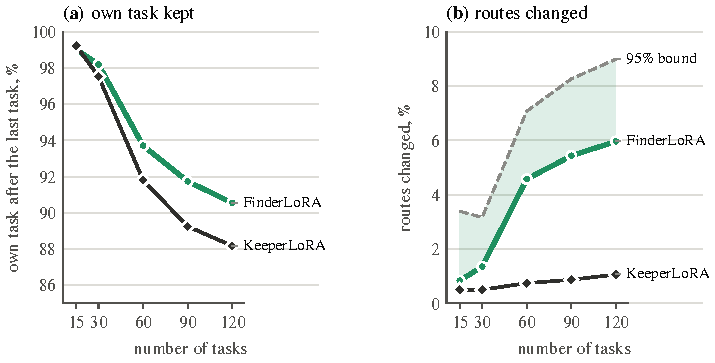
\includegraphics[width=\linewidth]{figures/recogniser_scale}
  \caption{Many tasks, routes only (frozen T5-base states). Left: share of test inputs given to their own task after the last task. Right: share of routes that changed after their task arrived, with the 95\% bound of the audit for \recog{}. The point at 15 tasks is the SuperNI benchmark; the others are 30, 60 and 90 fresh tasks and all 120 tasks together.}
  \label{fig:recogniserscale}
\end{figure}

\medskip
\noindent The per-task tables of this subsection follow.

\begin{table}[t]
  \caption{\recog{} (ridge $1\times$) per task, development data: the 15 SuperNI tasks of order 1 in the order of arrival, frozen T5-base states. Own task at arrival and at the end, route changed: \% of the test inputs of the task. Held-out: held-out inputs of the task whose route changed, of all its held-out inputs. Audit $H/m$ and 95\% bound: Proposition~\ref{prop:audit}, in \%.}
  \label{tab:recogniserpertask}
  \centering
  {\footnotesize\setlength{\tabcolsep}{3pt}\begin{tabular}{lrrrrrr}
    \toprule
    Task & \shortstack[r]{Sent to\\own task\\at arrival,\\\% $\uparrow$} & \shortstack[r]{Sent to\\own task\\at the end,\\\% $\uparrow$} & \shortstack[r]{Route\\changed,\\\% $\downarrow$} & Held-out & \shortstack[r]{Audit\\$H/m$, \%} & \shortstack[r]{95\% bound,\\\%} \\
    \midrule
    samsum & \AudPtOneArrive{} & \AudPtOneEnd{} & \AudPtOneChanged{} & \AudPtOneC{} of \AudPtOneM{} & \AudPtOneAuditEst{} & \AudPtOneBound{} \\
    sst2 & \AudPtTwoArrive{} & \AudPtTwoEnd{} & \AudPtTwoChanged{} & \AudPtTwoC{} of \AudPtTwoM{} & \AudPtTwoAuditEst{} & \AudPtTwoBound{} \\
    xsum & \AudPtThreeArrive{} & \AudPtThreeEnd{} & \AudPtThreeChanged{} & \AudPtThreeC{} of \AudPtThreeM{} & \AudPtThreeAuditEst{} & \AudPtThreeBound{} \\
    outcome extr. & \AudPtFourArrive{} & \AudPtFourEnd{} & \AudPtFourChanged{} & \AudPtFourC{} of \AudPtFourM{} & \AudPtFourAuditEst{} & \AudPtFourBound{} \\
    quoref & \AudPtFiveArrive{} & \AudPtFiveEnd{} & \AudPtFiveChanged{} & \AudPtFiveC{} of \AudPtFiveM{} & \AudPtFiveAuditEst{} & \AudPtFiveBound{} \\
    relation extr. & \AudPtSixArrive{} & \AudPtSixEnd{} & \AudPtSixChanged{} & \AudPtSixC{} of \AudPtSixM{} & \AudPtSixAuditEst{} & \AudPtSixBound{} \\
    multi-woz & \AudPtSevenArrive{} & \AudPtSevenEnd{} & \AudPtSevenChanged{} & \AudPtSevenC{} of \AudPtSevenM{} & \AudPtSevenAuditEst{} & \AudPtSevenBound{} \\
    personachat & \AudPtEightArrive{} & \AudPtEightEnd{} & \AudPtEightChanged{} & \AudPtEightC{} of \AudPtEightM{} & \AudPtEightAuditEst{} & \AudPtEightBound{} \\
    commonsenseqa & \AudPtNineArrive{} & \AudPtNineEnd{} & \AudPtNineChanged{} & \AudPtNineC{} of \AudPtNineM{} & \AudPtNineAuditEst{} & \AudPtNineBound{} \\
    diplomacy & \AudPtTenArrive{} & \AudPtTenEnd{} & \AudPtTenChanged{} & \AudPtTenC{} of \AudPtTenM{} & \AudPtTenAuditEst{} & \AudPtTenBound{} \\
    glucose & \AudPtElevenArrive{} & \AudPtElevenEnd{} & \AudPtElevenChanged{} & \AudPtElevenC{} of \AudPtElevenM{} & \AudPtElevenAuditEst{} & \AudPtElevenBound{} \\
    reddit tifu & \AudPtTwelveArrive{} & \AudPtTwelveEnd{} & \AudPtTwelveChanged{} & \AudPtTwelveC{} of \AudPtTwelveM{} & \AudPtTwelveAuditEst{} & \AudPtTwelveBound{} \\
    sciq & \AudPtThirteenArrive{} & \AudPtThirteenEnd{} & \AudPtThirteenChanged{} & \AudPtThirteenC{} of \AudPtThirteenM{} & \AudPtThirteenAuditEst{} & \AudPtThirteenBound{} \\
    sentiment140 & \AudPtFourteenArrive{} & \AudPtFourteenEnd{} & \AudPtFourteenChanged{} & \AudPtFourteenC{} of \AudPtFourteenM{} & \AudPtFourteenAuditEst{} & \AudPtFourteenBound{} \\
    emotion & \AudPtFifteenArrive{} & \AudPtFifteenEnd{} & \AudPtFifteenChanged{} & \AudPtFifteenC{} of \AudPtFifteenM{} & \AudPtFifteenAuditEst{} & \AudPtFifteenBound{} \\
    \bottomrule
\end{tabular}}

\end{table}

\begin{table}[t]
  \caption{\recog{} per task on the 15 Long Sequence tasks in order 3, all official test inputs, routes only: own task at arrival and at the end, route changed (\% of the test inputs of the task); held-out inputs whose route changed, of all; audit $H/m$ and 95\% bound (Proposition~\ref{prop:audit}); last column: own task at the end under \handicap{} ($\nu = 2$).}
  \label{tab:recogniserlongpertask}
  \centering
  {\footnotesize\setlength{\tabcolsep}{2.5pt}\begin{tabular}{lrrrrrrr}
    \toprule
    & \multicolumn{6}{c}{\recog{}} & \handicap{} \\
    \cmidrule(lr){2-7}
    Task & \shortstack[r]{Sent to\\own task\\at arrival,\\\% $\uparrow$} & \shortstack[r]{Sent to\\own task\\at the end,\\\% $\uparrow$} & \shortstack[r]{Route\\changed,\\\% $\downarrow$} & Held-out & \shortstack[r]{Audit\\$H/m$, \%} & \shortstack[r]{95\% bound,\\\%} & \shortstack[r]{Sent to\\own task\\at the end,\\\% $\uparrow$} \\
    \midrule
    yelp & \AudScaleLongPtOneArrive{} & \AudScaleLongPtOneEnd{} & \AudScaleLongPtOneChanged{} & \AudScaleLongPtOneC{} of \AudScaleLongPtOneM{} & \AudScaleLongPtOneAuditEst{} & \AudScaleLongPtOneBound{} & \AudScaleLongPtOneHEnd{} \\
    amazon & \AudScaleLongPtTwoArrive{} & \AudScaleLongPtTwoEnd{} & \AudScaleLongPtTwoChanged{} & \AudScaleLongPtTwoC{} of \AudScaleLongPtTwoM{} & \AudScaleLongPtTwoAuditEst{} & \AudScaleLongPtTwoBound{} & \AudScaleLongPtTwoHEnd{} \\
    mnli & \AudScaleLongPtThreeArrive{} & \AudScaleLongPtThreeEnd{} & \AudScaleLongPtThreeChanged{} & \AudScaleLongPtThreeC{} of \AudScaleLongPtThreeM{} & \AudScaleLongPtThreeAuditEst{} & \AudScaleLongPtThreeBound{} & \AudScaleLongPtThreeHEnd{} \\
    cb & \AudScaleLongPtFourArrive{} & \AudScaleLongPtFourEnd{} & \AudScaleLongPtFourChanged{} & \AudScaleLongPtFourC{} of \AudScaleLongPtFourM{} & \AudScaleLongPtFourAuditEst{} & \AudScaleLongPtFourBound{} & \AudScaleLongPtFourHEnd{} \\
    copa & \AudScaleLongPtFiveArrive{} & \AudScaleLongPtFiveEnd{} & \AudScaleLongPtFiveChanged{} & \AudScaleLongPtFiveC{} of \AudScaleLongPtFiveM{} & \AudScaleLongPtFiveAuditEst{} & \AudScaleLongPtFiveBound{} & \AudScaleLongPtFiveHEnd{} \\
    qqp & \AudScaleLongPtSixArrive{} & \AudScaleLongPtSixEnd{} & \AudScaleLongPtSixChanged{} & \AudScaleLongPtSixC{} of \AudScaleLongPtSixM{} & \AudScaleLongPtSixAuditEst{} & \AudScaleLongPtSixBound{} & \AudScaleLongPtSixHEnd{} \\
    rte & \AudScaleLongPtSevenArrive{} & \AudScaleLongPtSevenEnd{} & \AudScaleLongPtSevenChanged{} & \AudScaleLongPtSevenC{} of \AudScaleLongPtSevenM{} & \AudScaleLongPtSevenAuditEst{} & \AudScaleLongPtSevenBound{} & \AudScaleLongPtSevenHEnd{} \\
    imdb & \AudScaleLongPtEightArrive{} & \AudScaleLongPtEightEnd{} & \AudScaleLongPtEightChanged{} & \AudScaleLongPtEightC{} of \AudScaleLongPtEightM{} & \AudScaleLongPtEightAuditEst{} & \AudScaleLongPtEightBound{} & \AudScaleLongPtEightHEnd{} \\
    sst2 & \AudScaleLongPtNineArrive{} & \AudScaleLongPtNineEnd{} & \AudScaleLongPtNineChanged{} & \AudScaleLongPtNineC{} of \AudScaleLongPtNineM{} & \AudScaleLongPtNineAuditEst{} & \AudScaleLongPtNineBound{} & \AudScaleLongPtNineHEnd{} \\
    dbpedia & \AudScaleLongPtTenArrive{} & \AudScaleLongPtTenEnd{} & \AudScaleLongPtTenChanged{} & \AudScaleLongPtTenC{} of \AudScaleLongPtTenM{} & \AudScaleLongPtTenAuditEst{} & \AudScaleLongPtTenBound{} & \AudScaleLongPtTenHEnd{} \\
    agnews & \AudScaleLongPtElevenArrive{} & \AudScaleLongPtElevenEnd{} & \AudScaleLongPtElevenChanged{} & \AudScaleLongPtElevenC{} of \AudScaleLongPtElevenM{} & \AudScaleLongPtElevenAuditEst{} & \AudScaleLongPtElevenBound{} & \AudScaleLongPtElevenHEnd{} \\
    yahoo & \AudScaleLongPtTwelveArrive{} & \AudScaleLongPtTwelveEnd{} & \AudScaleLongPtTwelveChanged{} & \AudScaleLongPtTwelveC{} of \AudScaleLongPtTwelveM{} & \AudScaleLongPtTwelveAuditEst{} & \AudScaleLongPtTwelveBound{} & \AudScaleLongPtTwelveHEnd{} \\
    multirc & \AudScaleLongPtThirteenArrive{} & \AudScaleLongPtThirteenEnd{} & \AudScaleLongPtThirteenChanged{} & \AudScaleLongPtThirteenC{} of \AudScaleLongPtThirteenM{} & \AudScaleLongPtThirteenAuditEst{} & \AudScaleLongPtThirteenBound{} & \AudScaleLongPtThirteenHEnd{} \\
    boolq & \AudScaleLongPtFourteenArrive{} & \AudScaleLongPtFourteenEnd{} & \AudScaleLongPtFourteenChanged{} & \AudScaleLongPtFourteenC{} of \AudScaleLongPtFourteenM{} & \AudScaleLongPtFourteenAuditEst{} & \AudScaleLongPtFourteenBound{} & \AudScaleLongPtFourteenHEnd{} \\
    wic & \AudScaleLongPtFifteenArrive{} & \AudScaleLongPtFifteenEnd{} & \AudScaleLongPtFifteenChanged{} & \AudScaleLongPtFifteenC{} of \AudScaleLongPtFifteenM{} & \AudScaleLongPtFifteenAuditEst{} & \AudScaleLongPtFifteenBound{} & \AudScaleLongPtFifteenHEnd{} \\
    \bottomrule
\end{tabular}}

\end{table}


\subsection{Trained answers without instructions}
\label{sec:nodeftrained}

This subsection puts the recogniser in front of trained adapters and compares it with the two published methods of Section~\ref{sec:nodefpublished}, first on a small model and then on the model of the main runs. It uses the routes tested in Section~\ref{sec:recogniser}. The lines for each run were again fixed before it.

\paragraph{Trained answers on a small model.} The stand-alone code (\texttt{t5-small}, the five tasks, no definition in any input, one seed, on a CPU; first used for an earlier pilot reported in Section~\ref{sec:noinstruction}) was run with the routes of \recog{} on the frozen states of that small model, by the lines of that pilot: at most 20 of 200 answers changed and forgetting at most 3 points while more than 100 change with all adapters on; the score right after learning at least 90\% of that with all adapters on; at least 80\% of the test inputs at their own task.
With all adapters on, \AudSmallAllChanged{} of \AudSmallAllCompared{} answers to earlier tasks changed and the score fell from \AudSmallAllLearned{} to \AudSmallAllAP{}; with the routes, \AudSmallRidgeChanged{} of \AudSmallRidgeCompared{} changed, forgetting was \AudSmallRidgeFT{}, the score went from \AudSmallRidgeLearned{} to \AudSmallRidgeAP{}, and 97.2\% of the test inputs reached their own task: ``works''.
Two of the five tasks are learned poorly by this small model under either rule, so they add little to the comparison. This check was planned before the GPU run of the next paragraph and finished after it.

\paragraph{Trained answers: our method against the published methods, without instructions.} The same five-task run as in Section~\ref{sec:nodefpublished}, on a GPU, with plain adapters that are never blocked: while task $t$ is learned, adapters $1$ to $t$ are on for all its inputs, and at test time an input is answered by the adapters that existed when the task it is routed to was learned.
The routes of \recog{} and \handicap{} ($\nu = 2$), on the frozen T5-base states of the instance, were written to the repository before the run (Table~\ref{tab:routesgpu}, at the end of this subsection).
Line fixed before the run: ``beats the published methods in this setting'' if all three hold: the final score is at least 2 points above the better published method without definitions; forgetting is below 2 points; at most 32 of the \AudOursRidgeCompared{} compared answers change (a quarter of what GainLoRA changes).
``Does not'' if the final score is below that of the better published method or at least \AudPubGainloraNoDefChanged{} answers change; anything else is ``mixed''.
For \recog{} the final score is \AudOursRidgeAP{} against \AudPubGainloraNoDefAP{} for GainLoRA, forgetting is \AudOursRidgeFT{}, and \AudOursRidgeChanged{} of \AudOursRidgeCompared{} answers changed.
For \handicap{} the figures are \AudOursHandicapAP{}, \AudOursHandicapFT{} and \AudOursHandicapChanged{} of \AudOursHandicapCompared{}.
All three lines hold for both, so the verdict is ``beats the published methods in this setting''.
Our guesses for \recog{}, 5 to 15 changed answers and forgetting below 1 point, held; they were written before \handicap{} was added to the table.
Five things must be said with it.

(a) The line said ``official test'', but the official test scores the plain adapters with all of them on (final score \AudOffOursNoDefAP{}); the routed rules exist only in the re-test.
So the re-test is compared with the re-test.
The two scorings of the published methods differ little (\AudPubGainloraNoDefAP{} against \AudOffGainloraNoDefAP{} for GainLoRA, \AudPubInfloraNoDefAP{} against \AudOffInfloraNoDefAP{} for InfLoRA).

(b) At 10 epochs most of the gap in the final score is learning, not retention.
Our guess for the score right after learning was 54 to 58, because we assumed that our adapters would learn as poorly without definitions as the published methods do; it was far too low: it is \AudOursRidgeLearned{}.
Plain adapters learn the five tasks almost as well without the definitions (\AudOursAllLearned{}) as with them (\AudWordOriginalAllLearned{}), with sst2 at \AudOursPtLearnedSst{} and emotion at \AudOursPtLearnedEmotion{}, where the published methods reach \AudPubInfloraNoDefPtLearnedSst{} and \AudPubGainloraNoDefPtLearnedSst{} on sst2 and \AudPubInfloraNoDefPtLearnedEmotion{} and \AudPubGainloraNoDefPtLearnedEmotion{} on emotion (Table~\ref{tab:noinstpertask} in Section~\ref{sec:nodefpublished}).
These two methods restrict what a new adapter may change, to protect the old tasks, and with a tenth of their published number of epochs they learn two of the five tasks poorly; with their full number of epochs they learn them (the paragraph on \AudFullEpochs{} epochs below).
The columns that are about retention are forgetting and changed answers: \AudOursRidgeFT{} and \AudOursHandicapFT{} for ours against \AudPubGainloraNoDefFT{} and \AudPubInfloraNoDefFT{} for the published methods, and \AudOursRidgeChanged{} and \AudOursHandicapChanged{} changed answers against \AudPubGainloraNoDefChanged{} and \AudPubInfloraNoDefChanged{}.
These are less tied to learning than the final score, but not free of it: forgetting cannot exceed what was learned, and the answers of a method that has learned less may be less stable. The run of the published methods at their published number of epochs, below, separates the two.

(c) Our final score without any definition is also above the published methods with their definitions (\AudPubGainloraDefAP{} for GainLoRA and \AudPubInfloraDefAP{} for InfLoRA), with the same caveat on learning. We had expected GainLoRA with definitions to stay ahead of ours without them; it did not.

(d) The audit next to what happened (Table~\ref{tab:routesgpu}): over the first four tasks the audit of \recog{} says \AudRouteFiveRidgeFirstFourAuditEst{}\% of the routes changed on average, with 95\% bounds per task from \AudRouteFiveRidgeFirstFourBoundLow{}\% to \AudRouteFiveRidgeFirstFourBoundHigh{}\%; \AudRouteFiveRidgeChanged{} of their \AudRouteFiveRidgeCompared{} routes changed (\AudRouteFiveRidgeChangedShare{}\%). Each changed route changed its answer, and no other answer changed.
For \handicap{} it is \AudRouteFiveHandicapChanged{} of \AudRouteFiveHandicapCompared{}; the audit is not valid for it on the same held-out inputs (Remark~\ref{rem:auditlimits}(iii)).

(e) It is one sequence of five tasks and a small model: a first sign and no more. The published methods were run with their full number of epochs for one seed only (below). The five tasks are among the 15 on which the rule and its one setting were chosen, and that choice looked at the test inputs of those tasks; the choice was between variants that differ by at most 1.5 points there (Table~\ref{tab:recogniserdev} in Section~\ref{sec:recogniser}), but the routes of this run are in that sense development routes, and only the fresh batches test the recogniser on tasks it was not chosen on.

\paragraph{Three seeds.} After the first seed had been read, seeds 43 and 44 were run for the published methods and for ours (the route table does not depend on the seed; only the adapters differ).
Reading fixed before these runs: the verdict stands for three seeds if the three lines hold for the means over the seeds and the final score of \recog{} is above that of the better published method in every single seed.
Table~\ref{tab:noinstseeds} gives the means.
The final score of \recog{} is \AudSeedsRidgeAP{} (\AudSeedsRidgeAPLow{} to \AudSeedsRidgeAPHigh{} over the seeds) against \AudSeedsGainloraAP{} for GainLoRA and \AudSeedsInfloraAP{} for InfLoRA; its forgetting is \AudSeedsRidgeFT{} points, and \AudSeedsRidgeChanged{} of \AudSeedsCompared{} answers changed, against \AudSeedsGainloraChanged{} and \AudSeedsInfloraChanged{}.
\handicap{} ends at \AudSeedsHandicapAP{} with \AudSeedsHandicapChanged{} changed answers.
\recog{} is above the better published method in \AudSeedsRidgeAboveInAll{} of \AudSeedsN{} seeds, so the verdict stands for three seeds, with the same five things to be said.
Our guesses for these seeds (a final score of 76 to 79 in each, 4 to 9 changed answers of 400 for \recog{} and 0 to 3 for \handicap{}) held.
Our three seeds differ little, as expected, since the routes are the same in every seed.
The simpler rule \centre{} (the nearest centre of word-vectors of the whole input, Section~\ref{sec:method}) ends at \AudSeedsCentreAP{} with \AudSeedsCentreChanged{} changed answers: even this simple rule goes most of the way here; \recog{} and \handicap{} add about three points (the ceiling is \AudSeedsOwnAP{}), fewer changed answers, and the audit and the bound.

\paragraph{The published methods with their published number of epochs.} Point (b) left open whether the two published methods close the gap with their full training. So both were run once more without definitions with \AudFullEpochs{} epochs per task, the published number, on the same five tasks (seed 42, T5-base; Table~\ref{tab:noinstfull}).
Lines fixed before the run: ``they close the learning gap'' if the score right after learning reaches at least 73, within five points of ours with 10 epochs, and ``they do not'' below 65; ``they hold their answers less well than ours'' if forgetting is at least 5 points above ours or at least 60 more of the \AudFullCompared{} answers change than under \recog{}, and ``no such sign'' if forgetting is within 2 points of ours and at most 25 more answers change.
Both lines are met.
With \AudFullEpochs{} epochs the two methods learn the five tasks as well as plain adapters do with 10 (\AudFullInfloraLearned{} for InfLoRA and \AudFullGainloraLearned{} for GainLoRA right after learning, against \AudOursRidgeLearned{}), and a little less than plain adapters with \AudFullEpochs{} epochs (\AudFullOursRidgeLearned{}). They now learn sst2 and emotion, the two tasks they had learned poorly (Table~\ref{tab:noinstfullpertask}).
Then they lose them: forgetting is \AudFullInfloraFT{} and \AudFullGainloraFT{} points, \AudFullInfloraChanged{} and \AudFullGainloraChanged{} of \AudFullCompared{} answers change, and the final scores are \AudFullInfloraAP{} and \AudFullGainloraAP{}, against \AudOursRidgeAP{} for plain adapters behind \recog{} with a tenth of the epochs (\AudOursRidgeFT{} points of forgetting, \AudOursRidgeChanged{} changed answers) and \AudFullOursRidgeAP{} with the same number of epochs (next paragraph).
From 10 to \AudFullEpochs{} epochs their forgetting grew with what they had learned: from \AudPubInfloraNoDefFT{} to \AudFullInfloraFT{} points for InfLoRA and from \AudPubGainloraNoDefFT{} to \AudFullGainloraFT{} for GainLoRA.
So in this run the gap in the final score is forgetting and not learning; the first sentence of point (b) belongs to the comparison at 10 epochs.
Our guesses were partly wrong, and wrong in the direction of too little forgetting: we had expected them to learn 68 to 78 (right; InfLoRA is just above), to change 60 to 200 answers (right for GainLoRA, far too few for InfLoRA) and to forget 4 to 15 points (wrong for both).
One limit belongs to this run: it is one seed and five tasks on T5-base, where the published setting uses a larger model. Why the two methods lose their answers is the question of the control below.

\paragraph{Our rules with the same number of epochs.} The comparison above gives the published methods ten times the training of ours. So plain adapters were also trained for \AudFullEpochs{} epochs per task (seed 42, no definitions, the same route table; top of Table~\ref{tab:noinstfull}).
Line fixed before the run: ``beats the published methods at equal epochs, in this setting'' if the final score of \recog{} is at least 2 points above the better published method at \AudFullEpochs{} epochs, forgetting is below 2 points, and at most 44 of \AudFullCompared{} answers change (a quarter of what GainLoRA changes); ``does not'' if the final score is below that method's.
All three hold. \recog{} ends at \AudFullOursRidgeAP{}, \AudFullOursRidgeAboveGainlora{} points above GainLoRA, with \AudFullOursRidgeFT{} points of forgetting and \AudFullOursRidgeChanged{} changed answers; \handicap{} ends at \AudFullOursHandicapAP{} with \AudFullOursHandicapChanged{}.
Right after learning the three ways are close (\AudFullOursRidgeLearned{} for ours, \AudFullInfloraLearned{} and \AudFullGainloraLearned{} for the published methods), so at equal training the gap in the final score is retention.
Lemma~\ref{lem:route} said in advance that at most as many answers can change as routes: the routes do not depend on the adapters, so they are the routes of the 10-epoch run; here exactly as many answers changed as routes, \AudFullOursRidgeChanged{} under \recog{} and \AudFullOursHandicapChanged{} under \handicap{}. Ten times the training changed no further answer.
The forgetting of \recog{} is \AudFullOursRidgeFT{} points here against \AudOursRidgeFT{} with 10 epochs: the same inputs go to another task, and a wrong route costs more when the adapters are better.
Our guesses held (a score right after learning of 77 to 82, a final score within one point of it, 3 to 6 changed answers); our doubt that more epochs might not help plain adapters was wrong, the score right after learning rose by \AudFullOursLearnedGain{} points.
It is one seed and five tasks. Figure~\ref{fig:answergrid} shows the changed answers one by one, and Figure~\ref{fig:stageheat} the score of every task after every stage.

\begin{figure}[t]
  \centering
  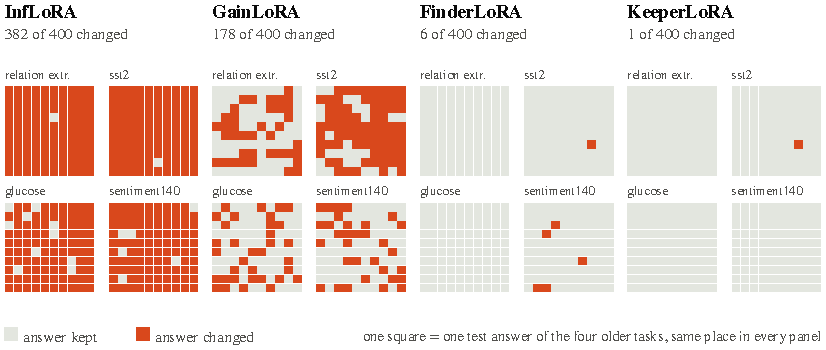
\includegraphics[width=\linewidth]{figures/answer_grid}
  \caption{Every square is one test answer. Five tasks without definitions, \AudFullEpochs{}
  epochs per task, seed 42: the \AudFullCompared{} test answers of the four older tasks, right
  after their task was learned against after the last task; a square has the same place in every
  panel. InfLoRA changes \AudFullInfloraChanged{} of the \AudFullCompared{} answers, GainLoRA
  \AudFullGainloraChanged{}, \recog{} \AudFullOursRidgeChanged{} and \handicap{}
  \AudFullOursHandicapChanged{}.}
  \label{fig:answergrid}
\end{figure}

\begin{figure}[t]
  \centering
  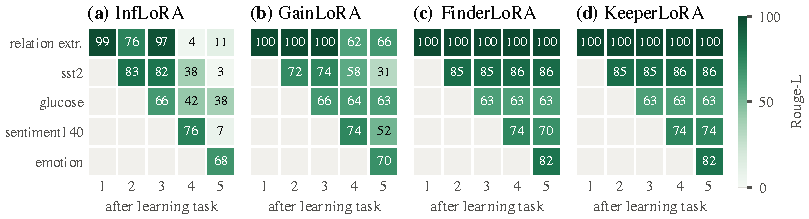
\includegraphics[width=\linewidth]{figures/stage_heatmap}
  \caption{The score of each task (rows) after each later task has been learned (columns), for the
  runs of Figure~\ref{fig:answergrid}; Rouge-L of the re-test (all reference answers), rounded. A
  row that keeps its colour is a task that is not forgotten: with InfLoRA and GainLoRA most rows of
  older tasks fade, with \recog{} and \handicap{} they stay.}
  \label{fig:stageheat}
\end{figure}


\paragraph{The control: the same methods with their definitions.} The run above cannot say by itself why the published methods lose their answers: the loss could come from the missing definition, or from \AudFullEpochs{} epochs on this smaller model. So the two methods were run once more with \AudFullEpochs{} epochs and the definitions left in; the seed, the tasks, the model and the code are the same, and the definition in the input is the only difference (Table~\ref{tab:fulldefinitions}).
Line fixed before the run, for each method: ``the instruction was what kept the answers'' if, with definitions, forgetting is at most half of its value without them and at most half as many answers change; ``it was not the instruction'' if forgetting with definitions is at least 80\% of that without.
The first holds for both. With definitions GainLoRA forgets \AudFullDefOriginalGainloraFT{} points and changes \AudFullDefOriginalGainloraChanged{} of \AudFullDefCompared{} answers, against \AudFullGainloraFT{} points and \AudFullGainloraChanged{} answers without; InfLoRA forgets \AudFullDefOriginalInfloraFT{} points and changes \AudFullDefOriginalInfloraChanged{} answers, against \AudFullInfloraFT{} and \AudFullInfloraChanged{}. The two differ in size: with their definitions GainLoRA holds nearly all its answers, InfLoRA fewer, so the instruction is what held most of their answers.
\recog{} and \handicap{}, which never read the definition, forget \AudFullOursRidgeFT{} and \AudFullOursHandicapFT{} points without it.
Two more things were to be reported as they are.
With their definitions and \AudFullEpochs{} epochs the two methods end at \AudFullDefOriginalInfloraAP{} (InfLoRA) and \AudFullDefOriginalGainloraAP{} (GainLoRA), below \cert{} and \recog{} with definitions and 10 epochs (\AudUOriginalCertAP{} and \AudUOriginalRidgeAP{}, Section~\ref{sec:exampleroutes}); we did not train our adapters for \AudFullEpochs{} epochs with definitions.
Under the heavy rewording they end at \AudFullDefHeavyInfloraAP{} and \AudFullDefHeavyGainloraAP{} with \AudFullDefHeavyInfloraChanged{} and \AudFullDefHeavyGainloraChanged{} changed answers (Table~\ref{tab:fullwordings}).
Our guesses were right for InfLoRA and for the forgetting of GainLoRA; GainLoRA learned less than we had guessed (\AudFullDefOriginalGainloraLearned{} right after learning, where we had said 79 to 84), and we had thought it more likely than not that it would end above our 10-epoch score, which it did not.
It is one seed and five tasks on T5-base. Figure~\ref{fig:learnkeep} puts the runs with and without definitions side by side.

\begin{figure}[t]
  \centering
  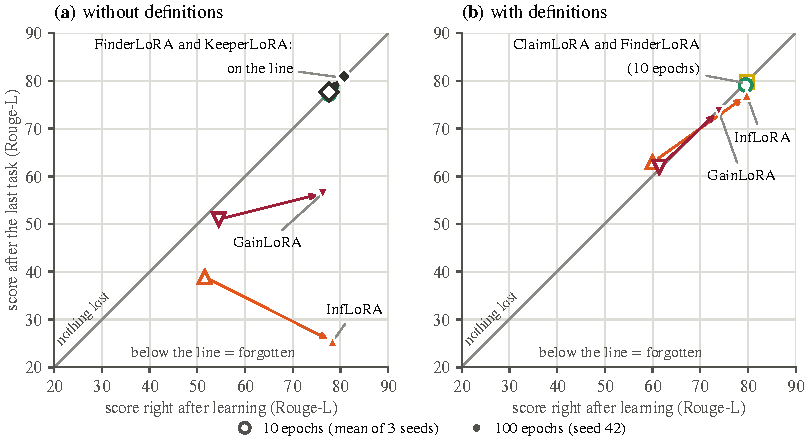
\includegraphics[width=\linewidth]{figures/learn_keep}
  \caption{Learned against kept, five tasks. A point is a method: its mean score right after
  learning ($x$) and after the last task ($y$). On the diagonal nothing is lost; the distance below
  it is what was forgotten. Hollow: 10 epochs (mean of three seeds); filled: \AudFullEpochs{} epochs
  (seed 42); an arrow goes from 10 to \AudFullEpochs{} epochs. (a)~Without definitions the two
  published methods learn more with more epochs and fall further below the diagonal; \recog{} and
  \handicap{} stay on it. (b)~With definitions the published methods stay near the diagonal (the
  control run); for our rules with definitions only 10-epoch runs exist.}
  \label{fig:learnkeep}
\end{figure}


\begin{table}[t]
  \caption{The definition as the only difference: the two published methods with \AudFullEpochs{} epochs per task, with their definitions and without them (five tasks, seed 42, T5-base, re-test), and \recog{} and \handicap{} without definitions at the same number of epochs.}
  \label{tab:fulldefinitions}
  \centering
  {\footnotesize\setlength{\tabcolsep}{3pt}\begin{tabular}{p{1.9in}lrrrr}
    \toprule
    Method (seed 42, 100 epochs) & Definitions & \shortstack[r]{Score right\\after\\learning $\uparrow$} & \shortstack[r]{Final\\score $\uparrow$} & \shortstack[r]{Forgetting\\(points) $\downarrow$} & \shortstack[r]{Answers\\changed\\of \AudFullDefCompared{} $\downarrow$} \\
    \midrule
    InfLoRA & with & \AudFullDefOriginalInfloraLearned{} & \AudFullDefOriginalInfloraAP{} & \AudFullDefOriginalInfloraFT{} & \AudFullDefOriginalInfloraChanged{} \\
    InfLoRA & none & \AudFullInfloraLearned{} & \AudFullInfloraAP{} & \AudFullInfloraFT{} & \AudFullInfloraChanged{} \\
    \midrule
    GainLoRA & with & \AudFullDefOriginalGainloraLearned{} & \AudFullDefOriginalGainloraAP{} & \AudFullDefOriginalGainloraFT{} & \AudFullDefOriginalGainloraChanged{} \\
    GainLoRA & none & \AudFullGainloraLearned{} & \AudFullGainloraAP{} & \AudFullGainloraFT{} & \AudFullGainloraChanged{} \\
    \midrule
    \recog{} (ours) & none & \AudFullOursRidgeLearned{} & \AudFullOursRidgeAP{} & \AudFullOursRidgeFT{} & \AudFullOursRidgeChanged{} \\
    \handicap{} (ours) & none & \AudFullOursHandicapLearned{} & \AudFullOursHandicapAP{} & \AudFullOursHandicapFT{} & \AudFullOursHandicapChanged{} \\
    \bottomrule
\end{tabular}}

\end{table}

\begin{table}[t]
  \caption{The two published methods with their definitions and \AudFullEpochs{} epochs per task under the four wordings of the definition (seed 42, re-test); below, for reference, \cert{} and \recog{} with definitions and 10 epochs (Table~\ref{tab:instanceroutes}).}
  \label{tab:fullwordings}
  \centering
  {\scriptsize\setlength{\tabcolsep}{2pt}\begin{tabular}{p{1.2in}rrrrrrrr}
    \toprule
    & \multicolumn{4}{c}{Final score $\uparrow$} & \multicolumn{4}{c}{\shortstack{Answers changed\\of \AudFullDefCompared{} $\downarrow$}} \\
    \cmidrule(lr){2-5}\cmidrule(l){6-9}
    & original & light & medium & heavy & original & light & medium & heavy \\
    \midrule
    InfLoRA, 100 epochs & \AudFullDefOriginalInfloraAP{} & \AudFullDefLightInfloraAP{} & \AudFullDefMediumInfloraAP{} & \AudFullDefHeavyInfloraAP{} & \AudFullDefOriginalInfloraChanged{} & \AudFullDefLightInfloraChanged{} & \AudFullDefMediumInfloraChanged{} & \AudFullDefHeavyInfloraChanged{} \\
    GainLoRA, 100 epochs & \AudFullDefOriginalGainloraAP{} & \AudFullDefLightGainloraAP{} & \AudFullDefMediumGainloraAP{} & \AudFullDefHeavyGainloraAP{} & \AudFullDefOriginalGainloraChanged{} & \AudFullDefLightGainloraChanged{} & \AudFullDefMediumGainloraChanged{} & \AudFullDefHeavyGainloraChanged{} \\
    \midrule
    \cert{}, 10 epochs & \AudUOriginalCertAP{} & \AudULightCertAP{} & \AudUMediumCertAP{} & \AudUHeavyCertAP{} & \AudUOriginalCertChanged{} & \AudULightCertChanged{} & \AudUMediumCertChanged{} & \AudUHeavyCertChanged{} \\
    \recog{}, 10 epochs & \AudUOriginalRidgeAP{} & \AudULightRidgeAP{} & \AudUMediumRidgeAP{} & \AudUHeavyRidgeAP{} & \AudUOriginalRidgeChanged{} & \AudULightRidgeChanged{} & \AudUMediumRidgeChanged{} & \AudUHeavyRidgeChanged{} \\
    \bottomrule
\end{tabular}}

\end{table}

\begin{table}[t]
  \caption{The five tasks without definitions, seed 42, T5-base, re-test: plain adapters behind \recog{} and \handicap{} and the two published methods, each with \AudFullEpochs{} epochs per task (the published number) and with 10. Score right after learning: average score right after each task was learned; Final score: average final score; Answers changed: answers to the test inputs of the first four tasks that differ at the end from the answer right after their task was learned.}
  \label{tab:noinstfull}
  \centering
  {\footnotesize\setlength{\tabcolsep}{3pt}\begin{tabular}{p{1.95in}rrrr}
    \toprule
    Method, epochs (seed 42, no definition) & \shortstack[r]{Score right\\after\\learning $\uparrow$} & \shortstack[r]{Final\\score $\uparrow$} & \shortstack[r]{Forgetting\\(points) $\downarrow$} & \shortstack[r]{Answers\\changed\\of \AudFullCompared{} $\downarrow$} \\
    \midrule
    \recog{} (ours), 100 epochs & \AudFullOursRidgeLearned{} & \AudFullOursRidgeAP{} & \AudFullOursRidgeFT{} & \AudFullOursRidgeChanged{} \\
    \handicap{} (ours), 100 epochs & \AudFullOursHandicapLearned{} & \AudFullOursHandicapAP{} & \AudFullOursHandicapFT{} & \AudFullOursHandicapChanged{} \\
    \midrule
    InfLoRA, 100 epochs & \AudFullInfloraLearned{} & \AudFullInfloraAP{} & \AudFullInfloraFT{} & \AudFullInfloraChanged{} \\
    GainLoRA, 100 epochs & \AudFullGainloraLearned{} & \AudFullGainloraAP{} & \AudFullGainloraFT{} & \AudFullGainloraChanged{} \\
    \midrule
    InfLoRA, 10 epochs & \AudPubInfloraNoDefLearned{} & \AudPubInfloraNoDefAP{} & \AudPubInfloraNoDefFT{} & \AudPubInfloraNoDefChanged{} \\
    GainLoRA, 10 epochs & \AudPubGainloraNoDefLearned{} & \AudPubGainloraNoDefAP{} & \AudPubGainloraNoDefFT{} & \AudPubGainloraNoDefChanged{} \\
    \midrule
    \recog{} (ours), 10 epochs & \AudOursRidgeLearned{} & \AudOursRidgeAP{} & \AudOursRidgeFT{} & \AudOursRidgeChanged{} \\
    \handicap{} (ours), 10 epochs & \AudOursHandicapLearned{} & \AudOursHandicapAP{} & \AudOursHandicapFT{} & \AudOursHandicapChanged{} \\
    \bottomrule
\end{tabular}}

\end{table}

\begin{table}[t]
  \caption{The two published methods without definitions with \AudFullEpochs{} epochs per task, seed 42, official test (one random reference answer): score of each task right after it was learned and after the last task.}
  \label{tab:noinstfullpertask}
  \centering
  {\footnotesize\setlength{\tabcolsep}{2pt}\begin{tabular}{lrr}
    \toprule
    & \multicolumn{2}{c}{\shortstack{Score right after\\learning $\to$ at the end $\uparrow$}} \\
    \cmidrule(l){2-3}
    Task & InfLoRA & GainLoRA \\
    \midrule
    relation extr. & \AudFullInfloraPtLearnedRelation{}\,$\to$\,\AudFullInfloraPtFinalRelation{} & \AudFullGainloraPtLearnedRelation{}\,$\to$\,\AudFullGainloraPtFinalRelation{} \\
    sst2 & \AudFullInfloraPtLearnedSst{}\,$\to$\,\AudFullInfloraPtFinalSst{} & \AudFullGainloraPtLearnedSst{}\,$\to$\,\AudFullGainloraPtFinalSst{} \\
    glucose & \AudFullInfloraPtLearnedGlucose{}\,$\to$\,\AudFullInfloraPtFinalGlucose{} & \AudFullGainloraPtLearnedGlucose{}\,$\to$\,\AudFullGainloraPtFinalGlucose{} \\
    sentiment140 & \AudFullInfloraPtLearnedSentiment{}\,$\to$\,\AudFullInfloraPtFinalSentiment{} & \AudFullGainloraPtLearnedSentiment{}\,$\to$\,\AudFullGainloraPtFinalSentiment{} \\
    emotion & \AudFullInfloraPtLearnedEmotion{}\,$\to$\,\AudFullInfloraPtFinalEmotion{} & \AudFullGainloraPtLearnedEmotion{}\,$\to$\,\AudFullGainloraPtFinalEmotion{} \\
    \bottomrule
\end{tabular}}

\end{table}

\begin{table}[t]
  \caption{The five tasks without definitions, means over \AudSeedsN{} seeds (42, 43, 44), re-test (every reference answer is used); T5-base, 10 epochs. Score right after learning: average score right after each task was learned. Final score: average final score, with the lowest and highest seed. Answers changed: answers to the test inputs of the first four tasks that differ at the end from the answer right after their task was learned, summed over the seeds. The last row sends every input to its own task. The route table of our rows is the same in every seed.}
  \label{tab:noinstseeds}
  \centering
  {\footnotesize\setlength{\tabcolsep}{2.5pt}\begin{tabular}{lrrrr}
    \toprule
    Method, no definition & \shortstack[r]{Score after\\learning $\uparrow$} & \shortstack[r]{Final\\score $\uparrow$} & \shortstack[r]{Forgetting\\(points) $\downarrow$} & \shortstack[r]{Answers changed\\of \AudSeedsCompared{} $\downarrow$} \\
    \midrule
    InfLoRA & \AudSeedsInfloraLearned{} & \AudSeedsInfloraAP{} {\scriptsize (\AudSeedsInfloraAPLow{}--\AudSeedsInfloraAPHigh{})} & \AudSeedsInfloraFT{} & \AudSeedsInfloraChanged{} \\
    GainLoRA & \AudSeedsGainloraLearned{} & \AudSeedsGainloraAP{} {\scriptsize (\AudSeedsGainloraAPLow{}--\AudSeedsGainloraAPHigh{})} & \AudSeedsGainloraFT{} & \AudSeedsGainloraChanged{} \\
    \midrule
    \plain{} & \AudSeedsPlainLearned{} & \AudSeedsPlainAP{} {\scriptsize (\AudSeedsPlainAPLow{}--\AudSeedsPlainAPHigh{})} & \AudSeedsPlainFT{} & \AudSeedsPlainChanged{} \\
    \centre{} & \AudSeedsCentreLearned{} & \AudSeedsCentreAP{} {\scriptsize (\AudSeedsCentreAPLow{}--\AudSeedsCentreAPHigh{})} & \AudSeedsCentreFT{} & \AudSeedsCentreChanged{} \\
    \recog{} (ours) & \AudSeedsRidgeLearned{} & \AudSeedsRidgeAP{} {\scriptsize (\AudSeedsRidgeAPLow{}--\AudSeedsRidgeAPHigh{})} & \AudSeedsRidgeFT{} & \AudSeedsRidgeChanged{} \\
    \handicap{} (ours) & \AudSeedsHandicapLearned{} & \AudSeedsHandicapAP{} {\scriptsize (\AudSeedsHandicapAPLow{}--\AudSeedsHandicapAPHigh{})} & \AudSeedsHandicapFT{} & \AudSeedsHandicapChanged{} \\
    own task (ceiling) & \AudSeedsOwnLearned{} & \AudSeedsOwnAP{} {\scriptsize (\AudSeedsOwnAPLow{}--\AudSeedsOwnAPHigh{})} & \AudSeedsOwnFT{} & \AudSeedsOwnChanged{} \\
    \bottomrule
\end{tabular}}

\end{table}

\begin{table}[t]
  \caption{Routes of the rules used in the GPU run, written before the run, for the five-task sequence (500 test inputs, 400 of the first four tasks compared) and for the 15 SuperNI tasks. Columns: test inputs not at their own task after the last task, out of all test inputs; routes that changed between the arrival of their task and the end, out of those compared; audit $H/m$ and 95\% bound (Proposition~\ref{prop:audit}, averaged over all tasks of the sequence, the last one included), where valid. The last row of each part sends every input to its own task.}
  \label{tab:routesgpu}
  \centering
  {\footnotesize\setlength{\tabcolsep}{3pt}\begin{tabular}{lrrrr}
    \toprule
    Rule & \shortstack[r]{Not sent\\to own task\\at the end $\downarrow$} & \shortstack[r]{Route\\changed $\downarrow$} & \shortstack[r]{Audit\\$H/m$, \%} & \shortstack[r]{95\% bound,\\\%} \\
    \midrule
    \multicolumn{5}{l}{\textit{five-task sequence}} \\
    \recog{} & \AudRouteFiveRidgeNotOwn{} of \AudRouteFiveRidgeN{} & \AudRouteFiveRidgeChanged{} of \AudRouteFiveRidgeCompared{} & \AudRouteFiveRidgeAuditEst{} & \AudRouteFiveRidgeAuditBound{} \\
    \handicap{}, $\nu = 2$ & \AudRouteFiveHandicapNotOwn{} of \AudRouteFiveHandicapN{} & \AudRouteFiveHandicapChanged{} of \AudRouteFiveHandicapCompared{} & -- & -- \\
    \recog{} with logistic regression & \AudRouteFiveJointNotOwn{} of \AudRouteFiveJointN{} & \AudRouteFiveJointChanged{} of \AudRouteFiveJointCompared{} & \AudRouteFiveJointAuditEst{} & \AudRouteFiveJointAuditBound{} \\
    every input to its own task (ceiling) & \AudRouteFiveOwnNotOwn{} of \AudRouteFiveOwnN{} & \AudRouteFiveOwnChanged{} of \AudRouteFiveOwnCompared{} & \AudRouteFiveOwnAuditEst{} & \AudRouteFiveOwnAuditBound{} \\
    \midrule
    \multicolumn{5}{l}{\textit{15 SuperNI tasks}} \\
    \recog{} & \AudRouteFifteenRidgeNotOwn{} of \AudRouteFifteenRidgeN{} & \AudRouteFifteenRidgeChanged{} of \AudRouteFifteenRidgeCompared{} & \AudRouteFifteenRidgeAuditEst{} & \AudRouteFifteenRidgeAuditBound{} \\
    \handicap{}, $\nu = 2$ & \AudRouteFifteenHandicapNotOwn{} of \AudRouteFifteenHandicapN{} & \AudRouteFifteenHandicapChanged{} of \AudRouteFifteenHandicapCompared{} & -- & -- \\
    \recog{} with logistic regression & \AudRouteFifteenJointNotOwn{} of \AudRouteFifteenJointN{} & \AudRouteFifteenJointChanged{} of \AudRouteFifteenJointCompared{} & \AudRouteFifteenJointAuditEst{} & \AudRouteFifteenJointAuditBound{} \\
    every input to its own task (ceiling) & \AudRouteFifteenOwnNotOwn{} of \AudRouteFifteenOwnN{} & \AudRouteFifteenOwnChanged{} of \AudRouteFifteenOwnCompared{} & \AudRouteFifteenOwnAuditEst{} & \AudRouteFifteenOwnAuditBound{} \\
    \bottomrule
\end{tabular}}

\end{table}

\paragraph{Fifteen tasks.} The same run was made on the 15 SuperNI tasks in their official order (seed 42, 10 epochs, no definitions; Table~\ref{tab:noinstfifteen}).
The published methods were not run on fifteen tasks without definitions, so the line fixed for that comparison cannot be read; what can be read is retention.
Plain adapters behind \recog{} end at \AudFifteenNoDefRidgeAP{}, \AudFifteenNoDefRidgeBelowOwn{} points below the ceiling of \AudFifteenNoDefOwnAP{}, with \AudFifteenNoDefRidgeFT{} points of forgetting and \AudFifteenNoDefRidgeChanged{} of \AudFifteenNoDefCompared{} changed answers; behind \handicap{} they end at \AudFifteenNoDefHandicapAP{} with \AudFifteenNoDefHandicapChanged{} changed answers.
The changed answers are exactly the routes that the route table changes; Lemma~\ref{lem:route} says that there can be at most that many.
With all adapters on, the same adapters end at \AudFifteenNoDefPlainAP{}, and every compared answer changes.
Our guesses (a score right after learning of 39 to 43, a final score within half a point of it, 8 to 20 changed answers) held.
For reference, with their definitions and the same number of epochs the two published methods ended at \AudFifteenDefGainloraAP{} (GainLoRA) and \AudFifteenDefInfloraAP{} (InfLoRA) on these tasks, with \AudFifteenDefGainloraChanged{} and \AudFifteenDefInfloraChanged{} changed answers (Section~\ref{sec:fifteen}); they had learned less there, so that gap is again partly learning.
The score right after learning is the same without definitions as with them (\AudFifteenNoDefOwnLearned{} and \AudFifteenDefCertLearned{}); the two averages agree by chance, the scores of the single tasks differ.
It is one seed, and these are the 15 tasks on which \recog{} was chosen. Figure~\ref{fig:routematrix} shows where the test inputs are sent after the last task.

\begin{figure}[t]
  \centering
  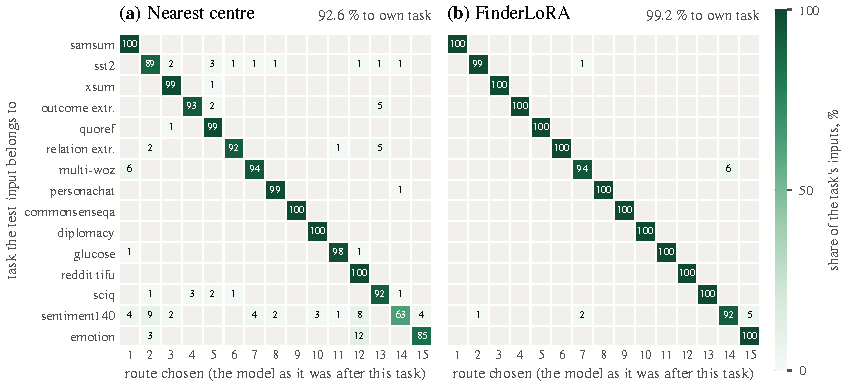
\includegraphics[width=\linewidth]{figures/route_matrix}
  \caption{Where the switch sends the test inputs: fifteen tasks without definitions, after the
  last task (seed 42). Rows: the task an input belongs to; columns: the route it gets; a cell is
  the share of the task's test inputs in per cent (shown from 1\,\%). (a)~The nearest centre sends
  \AudFifteenNoDefCentreRight{}\,\% of the inputs to their own task, (b)~\recog{}
  \AudFifteenNoDefRidgeRight{}\,\%.}
  \label{fig:routematrix}
\end{figure}


\begin{table}[t]
  \caption{The 15 SuperNI tasks without definitions, seed 42, T5-base, 10 epochs, re-test: the same plain adapters under each rule. Columns as in Table~\ref{tab:noinstfull}; the last column is the share of test inputs given to their own task after the last task. The three bottom rows are the run with definitions of Section~\ref{sec:fifteen}, for reference.}
  \label{tab:noinstfifteen}
  \centering
  {\footnotesize\setlength{\tabcolsep}{3pt}\begin{tabular}{p{1.75in}rrrrr}
    \toprule
    Method (seed 42, 15 tasks) & \shortstack[r]{Score right\\after\\learning $\uparrow$} & \shortstack[r]{Final\\score $\uparrow$} & \shortstack[r]{Forgetting\\(points) $\downarrow$} & \shortstack[r]{Answers\\changed\\of \AudFifteenNoDefCompared{} $\downarrow$} & \shortstack[r]{Sent to own\\task, \% $\uparrow$} \\
    \midrule
    \plain{} & \AudFifteenNoDefPlainLearned{} & \AudFifteenNoDefPlainAP{} & \AudFifteenNoDefPlainFT{} & \AudFifteenNoDefPlainChanged{} & \AudFifteenNoDefPlainRight{} \\
    \centre{} & \AudFifteenNoDefCentreLearned{} & \AudFifteenNoDefCentreAP{} & \AudFifteenNoDefCentreFT{} & \AudFifteenNoDefCentreChanged{} & \AudFifteenNoDefCentreRight{} \\
    \recog{} (ours) & \AudFifteenNoDefRidgeLearned{} & \AudFifteenNoDefRidgeAP{} & \AudFifteenNoDefRidgeFT{} & \AudFifteenNoDefRidgeChanged{} & \AudFifteenNoDefRidgeRight{} \\
    \handicap{} (ours) & \AudFifteenNoDefHandicapLearned{} & \AudFifteenNoDefHandicapAP{} & \AudFifteenNoDefHandicapFT{} & \AudFifteenNoDefHandicapChanged{} & \AudFifteenNoDefHandicapRight{} \\
    every input to its own task (ceiling) & \AudFifteenNoDefOwnLearned{} & \AudFifteenNoDefOwnAP{} & \AudFifteenNoDefOwnFT{} & \AudFifteenNoDefOwnChanged{} & \AudFifteenNoDefOwnRight{} \\
    \midrule
    \cert{}, with definitions & \AudFifteenDefCertLearned{} & \AudFifteenDefCertAP{} & \AudFifteenDefCertFT{} & \AudFifteenDefCertChanged{} & \AudFifteenDefCertRight{} \\
    GainLoRA, with definitions & \AudFifteenDefGainloraLearned{} & \AudFifteenDefGainloraAP{} & \AudFifteenDefGainloraFT{} & \AudFifteenDefGainloraChanged{} & -- \\
    InfLoRA, with definitions & \AudFifteenDefInfloraLearned{} & \AudFifteenDefInfloraAP{} & \AudFifteenDefInfloraFT{} & \AudFifteenDefInfloraChanged{} & -- \\
    \bottomrule
\end{tabular}}

\end{table}

\paragraph{What the results without instructions show.} This paragraph closes Sections~\ref{sec:nodefpublished}, \ref{sec:recogniser} and~\ref{sec:nodeftrained}. \emph{Reached:} without any instruction, a recogniser over all tasks that blocks nothing, stores one vector per task and one matrix for all tasks, and is the same for every order of arrival; on development data it gives \AudDevLLamOneEnd{}\% of the test inputs to their own task after 15 tasks. An audit and a bound in advance are proved (Proposition~\ref{prop:audit}, Theorem~\ref{thm:handicap}), and the measured change was within them in every run here (averages over tasks, one split each, and on the fresh batches a split that does not ensure exchangeability). Three rules passed their lines on fresh tasks, among them the \recog{} that was used on the GPU; it also passed its line on the second benchmark (\AudScaleLongThreeEnd{}\%, routes only) and still gives \AudScaleAllHundredTwentyEnd{}\% with 120 tasks. In one reduced setting, trained answers beat the two published methods that we ran without instructions, by the line fixed before (re-test against re-test). At 10 epochs most of the gap in the final score is learning; with their published \AudFullEpochs{} epochs (one seed) the two methods learn the tasks, and the gap is forgetting. The control with definitions at the same number of epochs says that the instruction is what held most of their answers (nearly all for GainLoRA, fewer for InfLoRA).
\emph{Not reached:} the published setting (a larger model; the full number of epochs was run for one seed only); the published methods on more than five tasks without definitions (ours ran on fifteen, one seed); the second benchmark with trained answers; a tight bound in advance; the published methods with an oracle for the task, or with our recogniser in front of them; the upper side of the conflict $\Omega$ (the error of the best classifier between two tasks); and inputs that occur in two tasks, which no method without instructions can do better than split.
Choices made after seeing numbers (the features, \handicap{} and its floor, the zone shapes) give development numbers; only the fresh batches and the GPU run were read once against lines written before.


The remaining subsections are mostly about inputs that carry an instruction: the certified switch \cert{} on five and on fifteen tasks, \recog{} with instructions, what the zones add and cost, and how the switch behaves under rewording, edits, other orders and other models; the last one returns to zones built without instructions.

\subsection{Five tasks with instructions: the certified switch}
\label{sec:five}

\begin{table}[t]
  \caption{Five-task sequence, original instructions (T5-base, 10 epochs per task; re-test against
  all reference answers). Score right after learning: average score of each task right after it was learned. AP:
  average score after the last task. Answers changed: test inputs of the first four
  tasks whose answer at the end differs from the answer given right after their task was learned.
  Certified: test inputs inside a zone.
  Scores are means over \FiveCertSeeds{} seeds, with the lowest and the highest seed in brackets; counts are summed over the seeds.}
  \label{tab:fivemain}
  \centering
  \small
  \setlength{\tabcolsep}{4pt}
  \begin{tabular}{lccccc}
    \toprule
    Method & \shortstack[c]{Score\\right after\\learning $\uparrow$} & \shortstack[c]{Final\\score $\uparrow$} & \shortstack[c]{Forgetting\\(points) $\downarrow$} & \shortstack[c]{Answers\\changed $\downarrow$} & Certified inputs \\
    \midrule
    \cert{} (ours) & 79.74 {\scriptsize(79.2--80.8)} & 79.74 {\scriptsize(79.2--80.8)} & 0.00 & 0 of 1{,}200 & 1{,}500 of 1{,}500 \\
    \nearest{} & 79.74 {\scriptsize(79.2--80.8)} & 79.74 {\scriptsize(79.2--80.8)} & 0.00 & 0 of 1{,}200 &  \\
    \centre{} & 79.74 {\scriptsize(79.2--80.8)} & 79.74 {\scriptsize(79.2--80.8)} & 0.00 & 0 of 1{,}200 &  \\
    \keyswitch{} & 79.74 {\scriptsize(79.2--80.8)} & 79.74 {\scriptsize(79.2--80.8)} & 0.00 & 0 of 1{,}200 &  \\
    \plain{} & 79.74 {\scriptsize(79.2--80.8)} & 36.08 {\scriptsize(32.3--39.5)} & 54.58 {\scriptsize(51.6--58.6)} & 994 of 1{,}200 &  \\
    \midrule
    InfLoRA & 60.02 {\scriptsize(56.6--63.3)} & 62.93 {\scriptsize(59.0--65.4)} & $-$3.14 {\scriptsize($-$5.3 to $-$1.7)} & 370 of 1{,}200 &  \\
    GainLoRA & 61.42 {\scriptsize(59.1--64.4)} & 61.96 {\scriptsize(60.9--63.9)} & $-$0.51 {\scriptsize($-$2.6 to 0.7)} & 65 of 1{,}200 &  \\
    \bottomrule
\end{tabular}

\end{table}

\begin{figure}[t]
  \centering
  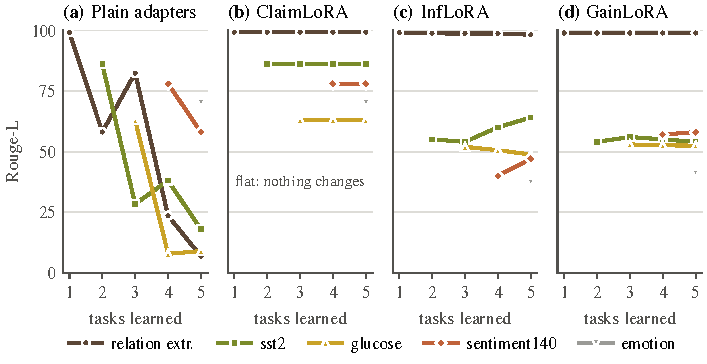
\includegraphics[width=\linewidth]{figures/five_tracks}
  \caption{Score of each of the five tasks as further tasks are learned (seed 42, original
  instructions). With plain adapters every task falls as soon as the next one is learned. With the
  certified switch the same adapters give flat lines. The two published methods are flat as well,
  at a lower level.}
  \label{fig:fivetracks}
\end{figure}

Table~\ref{tab:fivemain} and Figure~\ref{fig:fivetracks} give the result with instructions.

\paragraph{The certified switch keeps every answer.} With the certified switch the average score after the fifth task equals the
average score right after learning, \FiveCertAP{} Rouge-L. Forgetting is \FiveCertFT{}, and none of
the \FiveCertCompared{} answers to the test inputs of the first four tasks differs from the answer
that was given when the task had just been learned. All \FiveCertInputsOne{} test inputs lie inside
their own zone, as Proposition~\ref{prop:own} says they must, and no training input of a later
task lay inside an older zone (\FiveCertBlocked{} of \FiveCertTrainInputs{}). The outcome is therefore not an
observation about these runs but a consequence of Theorem~\ref{thm:writeonce}, and the experiment
confirms that the implementation does what the theorem describes. With the original instructions
\nearest{}, \centre{} and \keyswitch{} choose the same routes and give the same numbers.

\paragraph{The same adapters without a switch lose most of what they learned.} The rows from \cert{} to \plain{} use the same trained adapters; only the switches
differ. With all adapters on, the average falls from \FivePlainLearned{} right after learning to
\FivePlainAP{} at the end, forgetting is \FivePlainFT{} points, and \FivePlainChanged{} of
\FivePlainCompared{} answers change. Relation extraction, the first task, falls from
\FivePlainRelationLearned{} to \FivePlainRelationEnd{} on average over seeds (to 6.8 in the seed of
Figure~\ref{fig:fivetracks}a); only the task that was learned last is intact.

\paragraph{The published methods learned less here.} InfLoRA and GainLoRA have forgetting scores near zero on these five tasks
(\FiveInfFT{} and \FiveGainFT{} points; a
negative value means that old tasks improved on average while later ones were learned), though \FiveInfChanged{} and \FiveGainChanged{} of \FiveInfCompared{} answers change. Their curves
in Figure~\ref{fig:fivetracks} hardly fall. They nevertheless end at \FiveInfAP{}
and \FiveGainAP{}, well below the certified switch, because they are lower from the start: right
after learning, their tasks stand at \FiveInfLearned{} and \FiveGainLearned{} on average, against
\FiveCertLearned{} for plain adapters. Relation extraction is learned by both
(\FiveInfRelationLearned{} and \FiveGainRelationLearned{}). The classification tasks are not, within
ten epochs. On the two tasks with two labels the two methods are at the level of guessing right
after learning: \FiveInfSstLearned{} and \FiveGainSstLearned{} on SST-2 and
\FiveInfSentimentLearned{} and \FiveGainSentimentLearned{} on Sentiment140, where plain adapters
reach \FivePlainSstLearned{} and \FivePlainSentimentLearned{}; on emotion classification they stand
at \FiveInfEmotionLearned{} and \FiveGainEmotionLearned{} against \FivePlainEmotionLearned{}
(Table~\ref{tab:fivepertask} in the appendix). \textbf{So in our runs these two methods were at the level of guessing on two of the five tasks and clearly below plain adapters on a third, and the comparison cannot show how well they retain what they learn.} We do not know how much of this is the method and how much is our set-up: the budget is a
tenth of the published one, the model is smaller, and one step of both methods (a singular value
decomposition that the official code delegates to a library that did not load on the free GPUs) was
computed with PyTorch instead, without a check that the two agree number for number
(Appendix~\ref{app:impl}). A forgetting score at or
below zero also does not mean that nothing changes: \FiveInfChanged{} of \FiveInfCompared{} answers of
InfLoRA and \FiveGainChanged{} of \FiveGainCompared{} answers of GainLoRA are different at the end.
Changes for the better and for the worse cancel in the score.

\paragraph{The re-test agrees with the official test.} All numbers above come from the re-test, which scores every answer against all
reference answers. The scores written by the official script, which uses one randomly picked
reference per input, are \FiveCertOffAP{}, \FiveInfOffAP{} and \FiveGainOffAP{} for AP
(Table~\ref{tab:fiveofficial}) and lead to the same reading. With the original instructions the
re-test reproduced the answers of the official test on \FiveCertSame{} of \FiveCertSameOf{} inputs
for the certified switch, on \FiveInfSame{} of \FiveInfSameOf{} for InfLoRA and on \FiveGainSame{}
of \FiveGainSameOf{} for GainLoRA.

\paragraph{The same seed twice.} Seed 42 was run twice, in two separate sessions on the same kind
of GPU. For all three methods the first task was reproduced answer for answer (for the certified
switch and InfLoRA the second task as well), and the later tasks were not: for the certified
switch \RepeatCertSame{} of \RepeatCertTotal{} final
answers are the same, and the average score is \RepeatCertFirst{} in one run and
\RepeatCertSecond{} in the other (InfLoRA \RepeatInfFirst{} and \RepeatInfSecond{}, GainLoRA
\RepeatGainFirst{} and \RepeatGainSecond{}). Training is therefore not reproducible bit for bit on
this hardware, and differences of a few tenths of a point mean nothing. What does not vary is the
count for the certified switch: no answer of an earlier task changed in either run, nor in any
other seed. The tables use the second run of seed 42, which was made together with seeds 43
and 44.


\subsection{Reworded instructions}
\label{sec:reworded}

\begin{table}[t]
  \caption{Five tasks with the original and with reworded instructions: average score at the end and
  number of changed answers. The adapters are those of Table~\ref{tab:fivemain}; nothing is
  retrained. Means and sums over the seeds of Table~\ref{tab:fivemain}.}
  \label{tab:fivewordings}
  \centering
  \small
  \setlength{\tabcolsep}{4.5pt}
  \begin{tabular}{lcccccccc}
    \toprule
    & \multicolumn{4}{c}{Final score $\uparrow$} & \multicolumn{4}{c}{Answers changed (of 1{,}200) $\downarrow$} \\
    \cmidrule(lr){2-5} \cmidrule(lr){6-9}
    Method & original & light & medium & heavy & original & light & medium & heavy \\
    \midrule
    \cert{} (ours) & 79.7 & 79.6 & 79.0 & 74.1 & 0 & 0 & 0 & 0 \\
    \nearest{} & 79.7 & 79.6 & 79.0 & 74.1 & 0 & 0 & 0 & 0 \\
    \centre{} & 79.7 & 79.6 & 78.4 & 59.4 & 0 & 0 & 0 & 171 \\
    \keyswitch{} & 79.7 & 36.4 & 36.0 & 35.2 & 0 & 985 & 1{,}001 & 939 \\
    \plain{} & 36.1 & 36.4 & 36.0 & 35.2 & 994 & 985 & 1{,}001 & 939 \\
    \midrule
    InfLoRA & 62.9 & 64.3 & 57.8 & 54.3 & 370 & 296 & 320 & 470 \\
    GainLoRA & 62.0 & 64.6 & 58.8 & 51.6 & 65 & 58 & 122 & 178 \\
    \bottomrule
\end{tabular}

\end{table}

\begin{figure}[t]
  \centering
  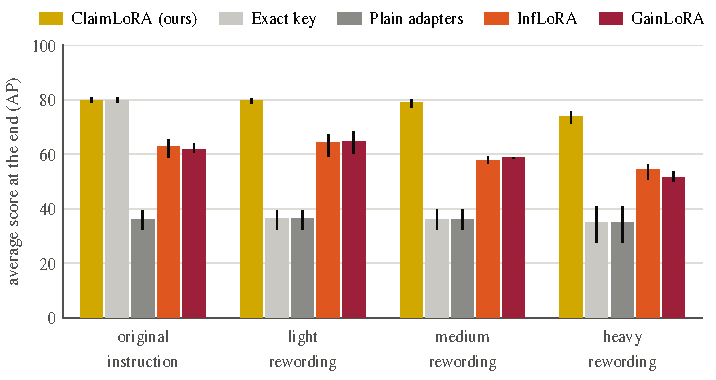
\includegraphics[width=0.9\linewidth]{figures/five_wordings}
  \caption{Average score at the end (AP) on the five tasks, with the original instructions and
  three levels of rewording. Bars are means over seeds; where there are several seeds a black line spans the lowest and the highest.}
  \label{fig:fivewordings}
\end{figure}

\begin{table}[t]
  \caption{Routes on the five tasks: how many test inputs are certified, how many are given to
  their own task, and how many answers change, for the certified switch and for the nearest-centre
  rule. Routes do not depend on the seed; counts are summed over seeds.}
  \label{tab:fiveroutes}
  \centering
  \small
  \setlength{\tabcolsep}{4.5pt}
  \begin{tabular}{lcccccc}
    \toprule
    & & \multicolumn{3}{c}{\cert{}} & \multicolumn{2}{c}{\centre{}} \\
    \cmidrule(lr){3-5} \cmidrule(lr){6-7}
    Wording & Tasks & Certified inputs & \shortstack[c]{Sent to own\\task $\uparrow$} & \shortstack[c]{Answers\\changed $\downarrow$} & \shortstack[c]{Sent to own\\task $\uparrow$} & \shortstack[c]{Answers\\changed $\downarrow$} \\
    \midrule
    original & 5 & 1{,}500 of 1{,}500 & 100.0\% & 0 of 1{,}200 & 100.0\% & 0 of 1{,}200 \\
    light & 5 & 1{,}500 of 1{,}500 & 100.0\% & 0 of 1{,}200 & 100.0\% & 0 of 1{,}200 \\
    medium & 5 & 300 of 1{,}500 & 100.0\% & 0 of 1{,}200 & 99.2\% & 0 of 1{,}200 \\
    heavy & 5 & 294 of 1{,}500 & 93.8\% & 0 of 1{,}200 & 72.2\% & 171 of 1{,}200 \\
    \bottomrule
\end{tabular}

\end{table}

A benchmark input carries its task definition word for word, so any rule that recognises the
definition looks perfect. The test that separates the rules is to ask the same task in other
words. Table~\ref{tab:fivewordings} and Figure~\ref{fig:fivewordings} repeat the evaluation with the
three rewordings of each definition, and Table~\ref{tab:fiveroutes} shows where the inputs go.

\paragraph{No answer changes under any wording.} For the certified switch the number of changed answers is zero in every column.
With the light rewording this is again guaranteed, because all \FiveCertZoneOneLight{} inputs are
still certified (Table~\ref{tab:fiveroutes}). With the medium and the heavy rewording it is not
guaranteed: only \FiveCertZoneOneMedium{} and \FiveCertZoneOneHeavy{} of the \FiveCertInputsOne{}
inputs are inside a zone, and they belong to relation extraction, the task with the longest
instruction. The other inputs kept their answers because no later task came nearer to them than
the task they had been given to, which Proposition~\ref{prop:uncertified} permits but does not
promise. It also depends on the order of the tasks: in an order in which SST-2 is learned after
Sentiment140, 31 routes of heavily reworded inputs would change when SST-2 arrives
(Section~\ref{sec:orders}). The average
score falls from \FiveCertAP{} with the original instructions to \FiveCertAPLight{},
\FiveCertAPMedium{} and \FiveCertAPHeavy{}.

\paragraph{An exact key is a lookup table.} \keyswitch{} compares the opening token for token. With the original instructions
it is perfect. With the light rewording, which changes a few words, it recognises nothing, leaves
all adapters on and ends at \FiveKeyAPLight{}, exactly where \plain{} ends. It fails because an
input that it does not recognise gets every adapter. \nearest{} and \cert{} send such an input to
the nearest zone instead, and they score alike on this benchmark; the radius of the zones decides
which of these inputs also carry the guarantee.

\paragraph{The nearest centre of the whole input fails under heavy rewording.} \centre{}, the nearest-centre rule with the token weights of Eq.~\eqref{eq:weights}, gives only
\FiveCentreRightHeavy{}\% of the heavily reworded inputs to their own task. Its score is
\FiveCentreAPHeavy{} against \FiveCertAPHeavy{}, and \FiveCentreChangedHeavy{} of
\FiveCentreComparedHeavy{} answers change as later tasks arrive. The first version of \cert{}, which used the nearest centre
with all tokens weighted equally, did better on these five tasks (97.4\% to the right task with seed 42, against
\FiveCertRightHeavy{}\% for the final rule) and was replaced because it failed on the 15-task sequence (Appendix~\ref{app:history}).

\paragraph{The published methods under rewording.} The published methods have no recognition step that a rewording could break, and
their forgetting scores stay within a few points in every wording, although many answers change (Table~\ref{tab:fivemore} in the
appendix). Their scores are \FiveInfAP{}, \FiveInfAPLight{}, \FiveInfAPMedium{} and
\FiveInfAPHeavy{} for InfLoRA and \FiveGainAP{}, \FiveGainAPLight{}, \FiveGainAPMedium{} and
\FiveGainAPHeavy{} for GainLoRA. The number of answers that differ at the end is largest under
heavy rewording, \FiveInfChangedHeavy{} and \FiveGainChangedHeavy{} of \FiveInfComparedHeavy{}.

\paragraph{Where the loss under heavy rewording comes from.} Under heavy rewording the certified switch scores \FiveCertAPHeavy{} instead of
\FiveCertAP{}. None of the difference is forgetting. One part is that the adapters themselves answer
a differently worded instruction less well: right after each task is learned, with all adapters on
(\plain{}), which at that moment is the right set of adapters, the score is
\FivePlainLearnedHeavy{}. The other part is routing:
\FiveCertWrongHeavy{} of the \FiveCertInputsOne{} heavily reworded inputs are given to another task,
which brings \FivePlainLearnedHeavy{} down to \FiveCertLearnedHeavy{}. All of them are tweets of the
Sentiment140 task that are given to SST-2, the other sentiment task.

\begin{figure}[t]
  \centering
  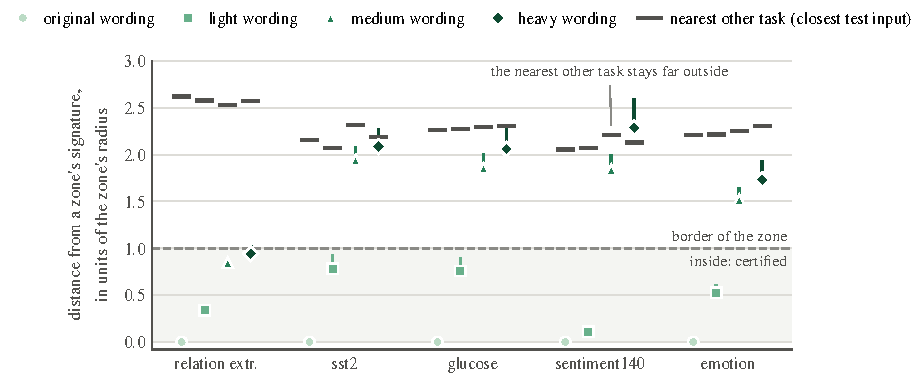
\includegraphics[width=0.92\linewidth]{figures/margins}
  \caption{Why rewording costs the certificate before it costs the route (five tasks, T5-base
  word-vectors). Markers: relative distance $\delta_k$ of the test inputs of a task from their own
  signature, in units of the radius of their own zone: median over the 100 inputs, with a line up to
  the farthest input. Short dark lines: how close the closest of these inputs comes to the signature of any
  \emph{other} task, in units of that task's radius. Below the dashed line an input is inside the
  zone, that is, certified.}
  \label{fig:margins}
\end{figure}

\paragraph{Where reworded inputs lie.}\label{sec:geometry} Figure~\ref{fig:margins} shows the geometry behind these numbers. With the original
wording every input lies exactly on the signature of its task (Proposition~\ref{prop:own}). The
light rewordings move the inputs by 0.1 to 0.8 radii, which is inside the zone. The medium and the
heavy rewordings move them by 1.5 to 2.3 radii in four of the five tasks, which is outside; relation
extraction, the task with the longest instruction, stays inside. The signatures of the other tasks,
however, are 2.1 to 2.6 of \emph{their} radii away from these inputs, so an input that has left its
zone is in most cases still nearer, in these units, to its own signature than to any other. The
certificate is lost long before the route is. The one place where the two margins cross is the
place of the errors: under the heavy rewording the tweets of Sentiment140 lie 2.29 radii from their
own signature (up to 2.60), and the signature of SST-2, the other sentiment task, is 2.13 of its
radii from the closest of them. Appendix~\ref{app:more} gives the numbers per task
(Table~\ref{tab:geometry}).

\subsection{Routes from the example alone: rewording cannot change the route}
\label{sec:exampleroutes}

The zones read the instruction, and a reworded instruction can leave them: under the heavy
rewording \cert{} sends some inputs to another task and ends below what the same adapters give
when every input reaches its own task (Section~\ref{sec:reworded}). \recog{} never
reads the instruction (Remark~\ref{rem:auditlimits}(v)). So the five tasks were trained once more
with their definitions (seed 42, plain adapters, nothing blocked), and the routes of \recog{} and
\handicap{} were computed from the example alone. It is the same route table as in the runs without
instructions (Section~\ref{sec:nodeftrained}), because these routes do not depend on the definition.
The scores of \cert{} equal those of the single-seed run of seed 42 with definitions, not those of the three-seed run of Table~\ref{tab:fivewordings} (seed 42 was trained twice; Section~\ref{sec:five}).
Line fixed before the run: \recog{} ``repairs the weak spot'' if its final score at the heavy
wording is at least 2 points above that of \cert{}, its score at the original wording is within
2 points of \cert{}, and at most 8 of the \AudUCompared{} compared answers change at every wording;
it ``does not'' if the heavy score is below that of \cert{} or the original score more than 4
points below.

\begin{table}[t]
  \caption{The five tasks with their definitions, seed 42, T5-base, 10 epochs, plain adapters; the
  same adapters under each rule, at the four wordings of the definition. Top: final score (AP,
  re-test). Bottom: answers to the test inputs of the first four tasks that differ at the end from
  the answer right after their task was learned, of \AudUCompared{}. \recog{} and \handicap{} set
  the route from the example alone; ``zone first'' uses the certified route where the input is
  inside a zone and the route of \recog{} or \handicap{} elsewhere. The rows of the published
  methods are from the run of the same seed in Section~\ref{sec:reworded}.}
  \label{tab:instanceroutes}
  \centering
  {\scriptsize\setlength{\tabcolsep}{2pt}\begin{tabular}{p{1.2in}rrrrrrrrr}
    \toprule
    & \multicolumn{4}{c}{Final score $\uparrow$} & \multicolumn{4}{c}{\shortstack{Answers changed\\of \AudUCompared{} $\downarrow$}} & \shortstack[r]{Sent to own\\task, heavy, \% $\uparrow$} \\
    \cmidrule(lr){2-5}\cmidrule(lr){6-9}
    & original & light & medium & heavy & original & light & medium & heavy & \\
    \midrule
    \cert{} (zones on the instruction) & \AudUOriginalCertAP{} & \AudULightCertAP{} & \AudUMediumCertAP{} & \AudUHeavyCertAP{} & \AudUOriginalCertChanged{} & \AudULightCertChanged{} & \AudUMediumCertChanged{} & \AudUHeavyCertChanged{} & \AudUHeavyCertRight{} \\
    \recog{} (example alone) & \AudUOriginalRidgeAP{} & \AudULightRidgeAP{} & \AudUMediumRidgeAP{} & \AudUHeavyRidgeAP{} & \AudUOriginalRidgeChanged{} & \AudULightRidgeChanged{} & \AudUMediumRidgeChanged{} & \AudUHeavyRidgeChanged{} & \AudUHeavyRidgeRight{} \\
    \handicap{}, $\nu = 2$ (example alone) & \AudUOriginalHandicapAP{} & \AudULightHandicapAP{} & \AudUMediumHandicapAP{} & \AudUHeavyHandicapAP{} & \AudUOriginalHandicapChanged{} & \AudULightHandicapChanged{} & \AudUMediumHandicapChanged{} & \AudUHeavyHandicapChanged{} & \AudUHeavyHandicapRight{} \\
    every input to its own task (ceiling) & \AudUOriginalOwnAP{} & \AudULightOwnAP{} & \AudUMediumOwnAP{} & \AudUHeavyOwnAP{} & \AudUOriginalOwnChanged{} & \AudULightOwnChanged{} & \AudUMediumOwnChanged{} & \AudUHeavyOwnChanged{} & \AudUHeavyOwnRight{} \\
    zone first, else \recog{} & \AudUOriginalMixRidgeAP{} & \AudULightMixRidgeAP{} & \AudUMediumMixRidgeAP{} & \AudUHeavyMixRidgeAP{} & \AudUOriginalMixRidgeChanged{} & \AudULightMixRidgeChanged{} & \AudUMediumMixRidgeChanged{} & \AudUHeavyMixRidgeChanged{} & \AudUHeavyMixRidgeRight{} \\
    zone first, else \handicap{} & \AudUOriginalMixHandicapAP{} & \AudULightMixHandicapAP{} & \AudUMediumMixHandicapAP{} & \AudUHeavyMixHandicapAP{} & \AudUOriginalMixHandicapChanged{} & \AudULightMixHandicapChanged{} & \AudUMediumMixHandicapChanged{} & \AudUHeavyMixHandicapChanged{} & \AudUHeavyMixHandicapRight{} \\
    \centre{} & \AudUOriginalCentreAP{} & \AudULightCentreAP{} & \AudUMediumCentreAP{} & \AudUHeavyCentreAP{} & \AudUOriginalCentreChanged{} & \AudULightCentreChanged{} & \AudUMediumCentreChanged{} & \AudUHeavyCentreChanged{} & \AudUHeavyCentreRight{} \\
    \plain{} & \AudUOriginalPlainAP{} & \AudULightPlainAP{} & \AudUMediumPlainAP{} & \AudUHeavyPlainAP{} & \AudUOriginalPlainChanged{} & \AudULightPlainChanged{} & \AudUMediumPlainChanged{} & \AudUHeavyPlainChanged{} & \AudUHeavyPlainRight{} \\
    \midrule
    GainLoRA & \AudWordOriginalGainloraAP{} & \AudWordLightGainloraAP{} & \AudWordMediumGainloraAP{} & \AudWordHeavyGainloraAP{} & \AudWordOriginalGainloraChanged{} & \AudWordLightGainloraChanged{} & \AudWordMediumGainloraChanged{} & \AudWordHeavyGainloraChanged{} & -- \\
    InfLoRA & \AudWordOriginalInfloraAP{} & \AudWordLightInfloraAP{} & \AudWordMediumInfloraAP{} & \AudWordHeavyInfloraAP{} & \AudWordOriginalInfloraChanged{} & \AudWordLightInfloraChanged{} & \AudWordMediumInfloraChanged{} & \AudWordHeavyInfloraChanged{} & -- \\
    \bottomrule
\end{tabular}}

\end{table}

Table~\ref{tab:instanceroutes} gives the result. At the heavy wording \recog{} ends at
\AudUHeavyRidgeAP{} and \handicap{} at \AudUHeavyHandicapAP{}, against \AudUHeavyCertAP{} for
\cert{} (seed 42; the mean over three seeds in Section~\ref{sec:reworded} is \FiveCertAPHeavy{});
the ceiling, with every input at its own task, is \AudUHeavyOwnAP{}. At the original
wording \recog{} ends at \AudUOriginalRidgeAP{} and \handicap{} at \AudUOriginalHandicapAP{},
against \AudUOriginalCertAP{}. At every wording \AudUOriginalRidgeChanged{} of \AudUCompared{}
answers change under \recog{} and \AudUOriginalHandicapChanged{} under \handicap{}, where \cert{}
changes none. All three lines hold: the verdict is ``repairs the weak spot''.
Our guesses (78.5 to 79.3 at the original wording, 75.5 to 76.7 at the heavy one) held, and one
was wrong in the good direction: we had expected about six changed answers for \recog{}, as in
the run without definitions. Six routes do change, but for three
of these inputs the model gives the same answer with the adapters up to either task. Without
definitions all six answers changed; why fewer change with the definition we did not test.

What this shows: the routes of \recog{} are the same at every wording, so its score stays
\AudURidgeBelowOwnLow{} to \AudURidgeBelowOwnHigh{} points below the ceiling at every wording
(\handicap{}: \AudUHandicapBelowOwnLow{} to \AudUHandicapBelowOwnHigh{} points), and what is lost
under rewording is what the adapters themselves lose when their instruction is reworded, not
misrouting. The zones are exact where the instruction is unedited and lose
\AudUHeavyCertBelowOwn{} points at the heavy wording through misrouted
inputs. The mixed rule has the best of both at the original, the light and the heavy wording; at
the medium wording it is below \cert{} (\AudUMediumMixRidgeAP{} and \AudUMediumMixHandicapAP{}
against \AudUMediumCertAP{}), whose own fallback is right for every input there. The published
methods end at \AudWordHeavyGainloraAP{} (GainLoRA) and \AudWordHeavyInfloraAP{} (InfLoRA) at the
heavy wording, with \AudWordHeavyGainloraChanged{} and \AudWordHeavyInfloraChanged{} changed
answers. This first run is one seed, five tasks, and three machine-written rewordings per task
that were looked at during development (Section~\ref{sec:protocol}), not
rewordings by people. Remark~\ref{rem:auditlimits}(v) says what this assumes about
the input.

\paragraph{Three seeds.} An independent reading of this result pointed out that seed 42 is the seed in which \cert{} loses most at the heavy wording. So the run was repeated for seeds 43 and 44 (Table~\ref{tab:instanceroutesseeds}).
Line fixed before these runs, for the means over the three seeds: the result ``stands for three seeds'' if the heavy score of \recog{} is at least 2 points above that of \cert{}, the original score is within 2 points of \cert{}, and in every seed at most 8 of \AudUCompared{} answers change at every wording.
It stands. At the heavy wording \recog{} ends at \AudUThreeHeavyRidgeAP{} and \handicap{} at \AudUThreeHeavyHandicapAP{}, against \AudUThreeHeavyCertAP{} for \cert{}, a gain of \AudUThreeHeavyRidgeAboveCert{} points; the ceiling is \AudUThreeHeavyOwnAP{}.
At the original wording \recog{} ends at \AudUThreeOriginalRidgeAP{}, \AudUThreeOriginalRidgeBelowCert{} points below \cert{} (\AudUThreeOriginalCertAP{}).
In no seed and at no wording do more than \AudUThreeMaxChangedPerSeed{} of \AudUCompared{} answers change under \recog{}.
Over the four wordings \recog{} stays \AudUThreeRidgeBelowOwnLow{} to \AudUThreeRidgeBelowOwnHigh{} points below the ceiling and \handicap{} \AudUThreeHandicapBelowOwnLow{} to \AudUThreeHandicapBelowOwnHigh{}; \cert{} loses \AudUThreeHeavyCertBelowOwn{} points at the heavy wording through misrouted inputs.
We had expected a smaller gain, 2 to 2.5 points: in seeds 43 and 44 the adapters themselves lose less under the heavy rewording than in seed 42.
These three seeds are not the training runs of Table~\ref{tab:fivewordings}: seed 42 is the single-seed run, and seeds 43 and 44 were trained again. So \cert{} ends at \AudUThreeOriginalCertAPOne{} (original) and \AudUThreeHeavyCertAPOne{} (heavy) here, and at \FiveCertAP{} and \FiveCertAPHeavy{} in Table~\ref{tab:fivewordings}; the difference is of the size seen between two runs of the same seed.
It remains five tasks, with machine-written rewordings that were looked at during development.

\begin{table}[t]
  \caption{As Table~\ref{tab:instanceroutes}, means over \AudUThreeSeeds{} seeds (42, 43, 44); changed answers are summed over the seeds. Training runs: seed 42 as in Table~\ref{tab:instanceroutes}, seeds 43 and 44 trained for this table; they are not the runs of Table~\ref{tab:fivewordings}, so the rows of \cert{} differ from it by a few tenths of a point.}
  \label{tab:instanceroutesseeds}
  \centering
  {\scriptsize\setlength{\tabcolsep}{2pt}\begin{tabular}{p{1.2in}rrrrrrrrr}
    \toprule
    & \multicolumn{4}{c}{Final score $\uparrow$} & \multicolumn{4}{c}{\shortstack{Answers changed\\of \AudUThreeCompared{} $\downarrow$}} & \shortstack[r]{Sent to own\\task, heavy, \% $\uparrow$} \\
    \cmidrule(lr){2-5}\cmidrule(lr){6-9}
    & original & light & medium & heavy & original & light & medium & heavy & \\
    \midrule
    \cert{} (zones on the instruction) & \AudUThreeOriginalCertAP{} & \AudUThreeLightCertAP{} & \AudUThreeMediumCertAP{} & \AudUThreeHeavyCertAP{} & \AudUThreeOriginalCertChanged{} & \AudUThreeLightCertChanged{} & \AudUThreeMediumCertChanged{} & \AudUThreeHeavyCertChanged{} & \AudUThreeHeavyCertRight{} \\
    \recog{} (example alone) & \AudUThreeOriginalRidgeAP{} & \AudUThreeLightRidgeAP{} & \AudUThreeMediumRidgeAP{} & \AudUThreeHeavyRidgeAP{} & \AudUThreeOriginalRidgeChanged{} & \AudUThreeLightRidgeChanged{} & \AudUThreeMediumRidgeChanged{} & \AudUThreeHeavyRidgeChanged{} & \AudUThreeHeavyRidgeRight{} \\
    \handicap{}, $\nu = 2$ (example alone) & \AudUThreeOriginalHandicapAP{} & \AudUThreeLightHandicapAP{} & \AudUThreeMediumHandicapAP{} & \AudUThreeHeavyHandicapAP{} & \AudUThreeOriginalHandicapChanged{} & \AudUThreeLightHandicapChanged{} & \AudUThreeMediumHandicapChanged{} & \AudUThreeHeavyHandicapChanged{} & \AudUThreeHeavyHandicapRight{} \\
    every input to its own task (ceiling) & \AudUThreeOriginalOwnAP{} & \AudUThreeLightOwnAP{} & \AudUThreeMediumOwnAP{} & \AudUThreeHeavyOwnAP{} & \AudUThreeOriginalOwnChanged{} & \AudUThreeLightOwnChanged{} & \AudUThreeMediumOwnChanged{} & \AudUThreeHeavyOwnChanged{} & \AudUThreeHeavyOwnRight{} \\
    zone first, else \recog{} & \AudUThreeOriginalMixRidgeAP{} & \AudUThreeLightMixRidgeAP{} & \AudUThreeMediumMixRidgeAP{} & \AudUThreeHeavyMixRidgeAP{} & \AudUThreeOriginalMixRidgeChanged{} & \AudUThreeLightMixRidgeChanged{} & \AudUThreeMediumMixRidgeChanged{} & \AudUThreeHeavyMixRidgeChanged{} & \AudUThreeHeavyMixRidgeRight{} \\
    zone first, else \handicap{} & \AudUThreeOriginalMixHandicapAP{} & \AudUThreeLightMixHandicapAP{} & \AudUThreeMediumMixHandicapAP{} & \AudUThreeHeavyMixHandicapAP{} & \AudUThreeOriginalMixHandicapChanged{} & \AudUThreeLightMixHandicapChanged{} & \AudUThreeMediumMixHandicapChanged{} & \AudUThreeHeavyMixHandicapChanged{} & \AudUThreeHeavyMixHandicapRight{} \\
    \centre{} & \AudUThreeOriginalCentreAP{} & \AudUThreeLightCentreAP{} & \AudUThreeMediumCentreAP{} & \AudUThreeHeavyCentreAP{} & \AudUThreeOriginalCentreChanged{} & \AudUThreeLightCentreChanged{} & \AudUThreeMediumCentreChanged{} & \AudUThreeHeavyCentreChanged{} & \AudUThreeHeavyCentreRight{} \\
    \plain{} & \AudUThreeOriginalPlainAP{} & \AudUThreeLightPlainAP{} & \AudUThreeMediumPlainAP{} & \AudUThreeHeavyPlainAP{} & \AudUThreeOriginalPlainChanged{} & \AudUThreeLightPlainChanged{} & \AudUThreeMediumPlainChanged{} & \AudUThreeHeavyPlainChanged{} & \AudUThreeHeavyPlainRight{} \\
    \midrule
    GainLoRA & \AudUThreeOriginalGainloraAP{} & \AudUThreeLightGainloraAP{} & \AudUThreeMediumGainloraAP{} & \AudUThreeHeavyGainloraAP{} & \AudUThreeOriginalGainloraChanged{} & \AudUThreeLightGainloraChanged{} & \AudUThreeMediumGainloraChanged{} & \AudUThreeHeavyGainloraChanged{} & -- \\
    InfLoRA & \AudUThreeOriginalInfloraAP{} & \AudUThreeLightInfloraAP{} & \AudUThreeMediumInfloraAP{} & \AudUThreeHeavyInfloraAP{} & \AudUThreeOriginalInfloraChanged{} & \AudUThreeLightInfloraChanged{} & \AudUThreeMediumInfloraChanged{} & \AudUThreeHeavyInfloraChanged{} & -- \\
    \bottomrule
\end{tabular}}

\end{table}


\subsection{Fifteen tasks with instructions}
\label{sec:fifteen}

The five-task sequence was chosen by us. To see whether the picture holds on a sequence that we did
not choose, we ran the 15 tasks of the official order~1 of Super-NaturalInstructions, with the same
model, budget and code, for the certified switch and for the two published methods. It is one seed,
and each run took 3.1 to 3.5 hours on a free GPU.

\begin{table}[t]
  \caption{Fifteen-task sequence, original instructions (T5-base, 10 epochs per task, seed 42;
  re-test against all reference answers). Columns as in Table~\ref{tab:fivemain}; ``Changed'' counts
  test inputs of the first 14 tasks. One seed.}
  \label{tab:fifteenmain}
  \centering
  \small
  \setlength{\tabcolsep}{4pt}
  \begin{tabular}{lccccc}
    \toprule
    Method & \shortstack[c]{Score\\right after\\learning $\uparrow$} & \shortstack[c]{Final\\score $\uparrow$} & \shortstack[c]{Forgetting\\(points) $\downarrow$} & \shortstack[c]{Answers\\changed $\downarrow$} & Certified inputs \\
    \midrule
    \cert{} (ours) & 42.77 & 42.77 & 0.00 & 0 of 1{,}097 & 1{,}197 of 1{,}197 \\
    \nearest{} & 42.77 & 42.77 & 0.00 & 0 of 1{,}097 &  \\
    \centre{} & 42.77 & 42.63 & 0.15 & 2 of 1{,}097 &  \\
    \keyswitch{} & 42.77 & 42.77 & 0.00 & 0 of 1{,}097 &  \\
    \plain{} & 42.77 & 14.88 & 30.67 & 973 of 1{,}097 &  \\
    \midrule
    InfLoRA & 30.46 & 26.13 & 5.69 & 661 of 1{,}097 &  \\
    GainLoRA & 29.08 & 28.62 & 1.09 & 215 of 1{,}097 &  \\
    \bottomrule
\end{tabular}

\end{table}

\begin{figure}[t]
  \centering
  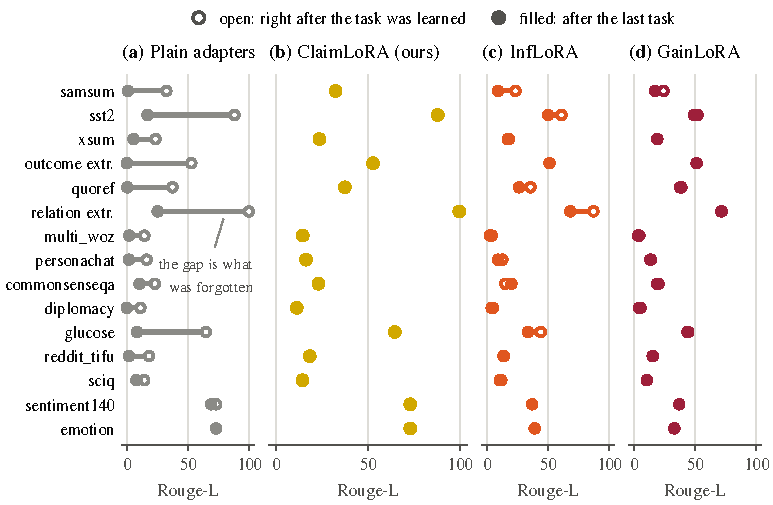
\includegraphics[width=\linewidth]{figures/fifteen_tasks}
  \caption{Score of each of the 15 tasks for four methods. Open circle: right after the task was
  learned. Filled circle: after the last task. A line between the two marks a change. For the
  certified switch the two circles coincide for every task.}
  \label{fig:fifteentasks}
\end{figure}

Table~\ref{tab:fifteenmain} and Figure~\ref{fig:fifteentasks} give the result. Appendix
Tables~\ref{tab:fifteenofficial} to \ref{tab:fifteenroutes} give the scores of the official script,
the scores for each wording, the scores of each task and the routes.

\paragraph{The certified switch keeps every answer.} The average score after the 15th task equals
the average score right after learning, \FifteenCertAP{} Rouge-L. Forgetting is \FifteenCertFT{},
and none of the \FifteenCertCompared{} answers to the test inputs of the first 14 tasks differs from
the answer given when the task had just been learned. All \FifteenCertInputsOne{} test inputs lie
inside their own zone, and no training input of a later task lay inside an older zone
(\FifteenCertBlocked{} of \FifteenCertTrainInputs{}). This is the outcome that Theorem~\ref{thm:writeonce}
guarantees. With the original instructions \nearest{} and \keyswitch{} give the same numbers, so
simpler rules reach the same score on this benchmark. \centre{} changes \FifteenCentreChanged{}
answers.

\paragraph{The same adapters without a switch lose most of what they learned.} With all adapters on,
the average falls from \FifteenPlainLearned{} to \FifteenPlainAP{}, forgetting is
\FifteenPlainFT{} points, and \FifteenPlainChanged{} of \FifteenPlainCompared{} answers change. The
score of every task except the last one falls (Table~\ref{tab:fifteenpertask} in the appendix).

\paragraph{The published methods learned less, and on fifteen tasks they also forget.} InfLoRA and
GainLoRA, run with their official code, end at \FifteenInfAP{} and \FifteenGainAP{}. On five tasks
neither forgot. Here InfLoRA forgets \FifteenInfFT{} points and GainLoRA \FifteenGainFT{}; the
answers that differ at the end are \FifteenInfChanged{} of \FifteenInfCompared{} for InfLoRA and
\FifteenGainChanged{} of \FifteenGainCompared{} for GainLoRA. The forgetting of InfLoRA is not
spread evenly. Relation extraction falls from \FifteenInfRelationLearned{} to
\FifteenInfRelationEnd{}, SST-2 from 61.0 to 50.0, summarisation of dialogues (SAMSum) from \FifteenInfSamsumLearned{} to
\FifteenInfSamsumEnd{} and Glucose from \FifteenInfGlucoseLearned{} to \FifteenInfGlucoseEnd{}. Both
methods also learned less right after each task: \FifteenInfLearned{} and \FifteenGainLearned{} on
average, against \FifteenCertLearned{} for plain adapters. So the gap of their final scores to the
certified switch has two parts, a gap in learning and a smaller gap from forgetting. We do not say
why they learned less. The caveats of the five-task runs apply: the budget is a tenth of the
published one, the model is smaller, and one step of their code was computed with a substitute
(Appendix~\ref{app:impl}). The official-script scores of InfLoRA are identical to those of an earlier run of the same method on Google Colab with the same seed, so for
this method the two platforms gave the same result (unlike the two five-task runs of seed 42, \fivefull{}).

\paragraph{The official script shows forgetting where no answer changed.} The official script gives
the certified switch an AP of \FifteenCertOffAP{} and a forgetting of \FifteenCertOffFT{}
(Table~\ref{tab:fifteenofficial}), although it changes no answer. This is evaluation noise, not
forgetting. The official script scores each answer against one reference answer, picked at random
on every load. The re-test, which scores every answer against all references, reproduces the
answers of the official test on \FifteenCertSame{} of \FifteenCertSameOf{} inputs for the certified
switch, \FifteenInfSame{} of \FifteenInfSameOf{} for InfLoRA and \FifteenGainSame{} of
\FifteenGainSameOf{} for GainLoRA, and it finds that none of the \FifteenCertCompared{} answers of
the certified switch changed. When the claim is that nothing changed, the answers have to be
compared and not the scores. The official scores of InfLoRA and GainLoRA lead to the same reading as
the re-test (AP \FifteenInfOffAP{} and \FifteenGainOffAP{}).

\begin{table}[t]
  \caption{Fifteen-task sequence with the original and with reworded instructions. The five tasks
  that have rewordings are those of the five-task sequence; they sit inside the 15-task sequence.
  AP is the average score of these five tasks after the last task, and ``Answers changed'' counts
  the test inputs of the first four of them (of 400); in the column ``original'' it counts those of the first 14 tasks (of 1{,}097). The adapters are those of Table~\ref{tab:fifteenmain};
  nothing is retrained. The column ``original'' is the whole sequence of 15 tasks.}
  \label{tab:fifteenwordings}
  \centering
  \small
  \setlength{\tabcolsep}{3.5pt}
  \begin{tabular}{lcccccccc}
    \toprule
    & \multicolumn{4}{c}{Final score $\uparrow$} & \multicolumn{4}{c}{Answers changed $\downarrow$} \\
    \cmidrule(lr){2-5} \cmidrule(lr){6-9}
    Method & original & light & medium & heavy & original & light & medium & heavy \\
    \midrule
    \cert{} (ours) & 42.8 & 80.7 & 80.2 & 76.0 & 0 & 0 & 0 & 0 \\
    \nearest{} & 42.8 & 80.7 & 80.2 & 76.0 & 0 & 0 & 0 & 0 \\
    \centre{} & 42.6 & 80.7 & 72.0 & 57.5 & 2 & 0 & 29 & 100 \\
    \keyswitch{} & 42.8 & 39.6 & 40.4 & 36.1 & 0 & 316 & 313 & 310 \\
    \plain{} & 14.9 & 39.6 & 40.4 & 36.1 & 973 & 316 & 313 & 310 \\
    \midrule
    InfLoRA & 26.1 & 51.6 & 44.7 & 32.6 & 661 & 257 & 272 & 270 \\
    GainLoRA & 28.6 & 51.1 & 47.1 & 37.0 & 215 & 69 & 85 & 109 \\
    \bottomrule
\end{tabular}

\end{table}

\paragraph{Reworded instructions inside the long sequence.} Table~\ref{tab:fifteenwordings} repeats
the five-task test inside the 15-task sequence. For the certified switch the number of changed
answers is zero in every wording. The average score of the five tasks is \FifteenCertAPLight{},
\FifteenCertAPMedium{} and \FifteenCertAPHeavy{} for the light, medium and heavy rewording. The
guarantee covers all \FifteenCertZoneOneLight{} inputs of the light rewording. For the medium and
the heavy rewording only \FifteenCertZoneOneMedium{} and \FifteenCertZoneOneHeavy{} of
\FifteenCertInputsOneMedium{} inputs are inside a zone, so the zero is again not guaranteed there.
\FifteenCertRightLight{}\%, \FifteenCertRightMedium{}\% and \FifteenCertRightHeavy{}\% of the inputs
are given to their own task. The exact key ends where plain adapters end (\FifteenPlainAPLight{},
\FifteenPlainAPMedium{}, \FifteenPlainAPHeavy{}). The nearest-centre rule \centre{} fails here: it gives \FifteenCentreRightMedium{}\% and
\FifteenCentreRightHeavy{}\% of the inputs with medium and heavy rewording to their own task, and
\FifteenCentreChangedMedium{} and \FifteenCentreChangedHeavy{} of \FifteenCentreComparedHeavy{}
answers change. InfLoRA forgets \FifteenInfFTLight{} points with the light rewording and
\FifteenInfFTHeavy{} with the heavy one on these five tasks, GainLoRA \FifteenGainFTLight{} and
\FifteenGainFTHeavy{} (Table~\ref{tab:fifteenmore} in the appendix). These rewordings are the
machine-written development set (Section~\ref{sec:protocol}); this run does not make
them an independent test.


\subsection{Where the gap to the published methods comes from}
\label{sec:gap}

\begin{figure}[t]
  \centering
  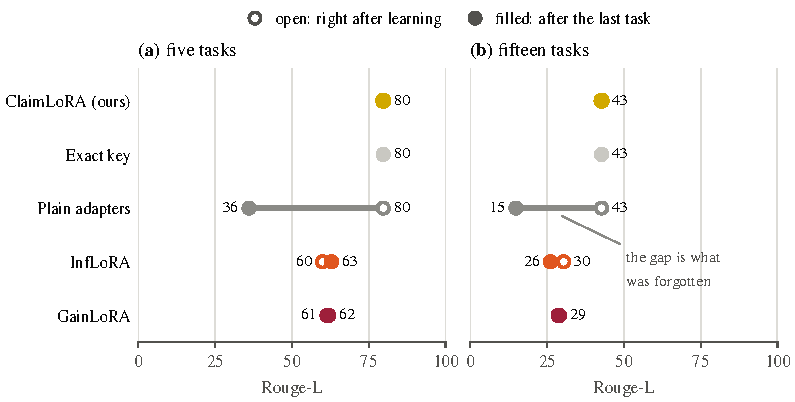
\includegraphics[width=0.9\linewidth]{figures/learn_forget}
  \caption{Learning and forgetting side by side, (a) on five tasks (mean over three seeds) and (b)
  on fifteen tasks (one seed). Open circle: average score of each task right
  after it was learned. Filled circle: average score after the last task. A gap between the two circles
  of a method is forgetting; an open circle far to the left is a lack of learning.}
  \label{fig:learnforget}
\end{figure}

Figure~\ref{fig:learnforget} separates the two things that a final score mixes.
For plain adapters the open circle is high and the filled circle is low: they learn and then forget.
For the two published methods on five tasks both circles are low and nearly equal: their forgetting scores are
near zero, but within ten epochs they have learned less. On fifteen tasks (panel b) their open circles are low
as well, and the filled circles are lower than the open ones for InfLoRA (\FifteenInfLearned{} to
\FifteenInfAP{}) and, by less, for GainLoRA (\FifteenGainLearned{} to \FifteenGainAP{}). The
certified switch has the open circle of plain adapters and no gap. On five tasks the comparison
therefore does not show that the published methods forget, and we do not claim that it does. On
fifteen tasks it shows some forgetting, and a larger lack of learning. In both, in our
set-up they had learned less by the time the next task arrived, for reasons we did not
separate (the method, the short budget, or our set-up), while the switch leaves the training of an
adapter untouched. The published results of both methods were
obtained with 100 epochs and T5-large. We could not run that setting, and the gap in learning may
well close there. Without instructions the same two methods did forget more
(Section~\ref{sec:nodefpublished}), with the same caveat on learning.


\subsection{What the zones add: a later task that looks like an old one}
\label{sec:stress}

On the benchmark sequences \nearest{} and \cert{} give the same routes, so the experiments above
cannot show what the frozen zones and the priority of older tasks are for. They matter when a later
task resembles an earlier one. We construct this case from the five-task sequence, at the level of
routes, which needs no GPU: after the five tasks a sixth task arrives whose inputs are of the same
kind as those of task~2 (SST-2 sentences) and whose definition is one of the rewordings of task~2's
definition. This is what happens when someone adds ``the same task again'' with a slightly
different instruction and possibly different labels. Table~\ref{tab:stress} counts how many of the
100 old test inputs of task~2, under each wording, are routed differently after the sixth task has
been added.

\begin{table}[t]
  \caption{Stress test (routes only, T5-base word-vectors). A sixth task with SST-2 inputs and a
  reworded SST-2 definition is added after the five tasks. ``Blocked'': training
  inputs of the new task that lie inside an older zone, reported when the task arrives. ``Routes
  changed'': old test inputs of task~2 (100 per wording) that are given to a different task
  afterwards.}
  \label{tab:stress}
  \centering
  \small
  \setlength{\tabcolsep}{4pt}
  \begin{tabular}{lccccccccc}
    \toprule
    & & \multicolumn{4}{c}{Routes changed, \cert{} $\downarrow$} & \multicolumn{4}{c}{Routes changed, \nearest{} $\downarrow$} \\
    \cmidrule(lr){3-6} \cmidrule(lr){7-10}
    New task's definition & Blocked & original & light & medium & heavy & original & light & medium & heavy \\
    \midrule
    light & 799 of 800 & 0 & 0 & 0 & 0 & 0 & 100 & 0 & 0 \\
    medium & 0 of 800 & 0 & 0 & 100 & 2 & 0 & 0 & 100 & 2 \\
    heavy & 0 of 800 & 0 & 0 & 0 & 100 & 0 & 0 & 0 & 100 \\
    \bottomrule
\end{tabular}

\end{table}

\paragraph{A look-alike inside an old zone is blocked and reported.} If the definition of the new
task is the light rewording of task~2's definition, its inputs fall inside the zone of task~2: 799 of
its 800 training inputs are blocked. The user is told so when the task arrives, before any
training. Under \cert{} not a single old input changes its route. Under \nearest{} the picture is
different: the old inputs with the light rewording, which task~2 has answered until now, carry the
instruction of the new task word for word and lie exactly on its signature, and all 100 are
re-routed to it. The same text gets a different answer from then on, and nothing announces it.
This is the case the frozen zones exist for: under a rule that always picks the best match, the
arrival of a task can change answers that were given before; under the oldest-claim rule it
cannot, for a certified input. Section~\ref{sec:paraphrase} counts how often this occurs among \WidenTasksEval{} real tasks with machine-paraphrased instructions: rarely, and the zones did not prevent it there (\nearest{} and \cert{} changed the same \RerouteNearNChanged{} of \RerouteInputs{} routes), so this constructed case is not typical of that collection. Whether the old or the new task ought to answer such a text is a question the rules do not
settle. The test is one constructed case and it is about routes; no adapter was trained for the
sixth task.

\paragraph{A look-alike outside every zone can take uncertified inputs.} If the new definition is
the medium or the heavy rewording, the new signature lies outside the zone of task~2. Nothing is
blocked, the new task gets a zone of its own, and under both rules the old inputs that carry exactly
that rewording are re-routed (100 of 100, plus 2 inputs with the heavy wording in the medium case).
Those inputs were never certified. The certified inputs of task~2, the original and the light
wording, keep their route in every case. The stress test thus shows both sides of the guarantee:
it protects exactly the certified inputs, and it does not protect the others.


\subsection{What the zones cost: 875 real tasks}
\label{sec:many}

The stress test built one look-alike task by hand. A large collection of real tasks contains
look-alikes by itself, and it shows how often the price of the guarantee has to be paid. We take
the \ManyTasks{} tasks of the default English split of Super-NaturalInstructions
\citep{wang2022superni}, each with its definition and its first inputs (\ManyInputs{} inputs;
openings of \ManyOpeningMin{} to \ManyOpeningMax{} tokens, \ManyOpeningMedian{} in the middle; the longest, \ManyOpeningMax{}, is the truncation length, so for these tasks the instance is cut off), let
them arrive in a random order, and give each task its zone when it arrives. No model is trained;
the test is about routes. Its rules, including what would count against the method, were fixed
before it was run (Appendix~\ref{app:many}).

\begin{table}[t]
  \caption{The zones on \ManyTasks{} real tasks arriving in a random order (routes only, T5-base
  word-vectors, unedited instructions). ``Blocked'': inputs of a new task that lie inside an older
  zone when the task arrives; the columns count the tasks for which this holds for none, some or all
  of their inputs. ``Routes changed later'': inputs that are given to a different task
  than right after their own task arrived, under \cert{} / \exactfirst{} / \nearest{}.}
  \label{tab:many}
  \centering
  \small
  \setlength{\tabcolsep}{4pt}
  \begin{tabular}{rccccccc}
    \toprule
    & \multicolumn{3}{c}{Tasks with blocked inputs} & \multicolumn{3}{c}{Inputs to their own task, \%} & Routes \\
    \cmidrule(lr){2-4} \cmidrule(lr){5-7}
    Tasks & none & some & all & \cert{} & \exactfirst{} & \nearest{} & changed later \\
    \midrule
    50 & 49 & 1 & 0 & 98.7 & 100.0 & 100.0 & 0 / 0 / 0 \\
    100 & 96 & 3 & 1 & 96.7 & 100.0 & 100.0 & 0 / 0 / 0 \\
    200 & 178 & 7 & 15 & 90.4 & 99.0 & 98.5 & 0 / 0 / 0 \\
    400 & 337 & 13 & 50 & 85.7 & 99.2 & 99.0 & 0 / 0 / 0 \\
    875 & 724 & 22 & 129 & 83.8 & 98.4 & 98.3 & 0 / 0 / 0 \\
    \bottomrule
\end{tabular}

\end{table}

\begin{figure}[t]
  \centering
  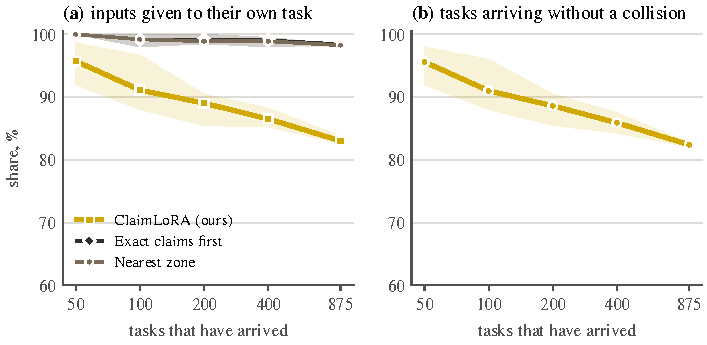
\includegraphics[width=0.86\linewidth]{figures/many}
  \caption{The price of the guarantee as the collection grows (same test as
  Table~\ref{tab:many}; lines are means over five random orders of arrival, bands span the lowest
  and the highest). (a) Share of inputs that are given to their own task; the variant of
  Section~\ref{sec:exactfirst} and the nearest-zone rule nearly coincide. (b) Share of tasks that
  arrive with no input inside an older zone.}
  \label{fig:many}
\end{figure}

\paragraph{The guarantee holds, and its price grows with the collection.} No certified input changed
its route, in any order of arrival and at any size of the collection. But the larger the
collection, the more often a new task arrives inside an older zone (Table~\ref{tab:many},
Figure~\ref{fig:many}). After all \ManyTasks{} tasks, \ManyColliding{} of them
(\ManyCollidingPct{}\%) have collided with an older task, and for \ManyAllHeld{} every input is
blocked, so that under their given instruction they could not be learned at all. In four other
random orders between \ManyCollidingPctLow{}\% and \ManyCollidingPctHigh{}\% of the tasks collide,
and in the order of the task numbers \ManyNumericCollidingPct{}\%. These collisions are not
accidents of the geometry. Of the \ManyColliding{} colliding tasks, \ManySameText{} have the same
definition text as the task they collide with, a further \ManyAlikeHigh{} share at least 80\% of its words,
and none shares less than \ManyAlikeLowest{}\%. They come from families
of tasks whose definitions differ in a word or two: \ManyFamilyMmlu{} are subject variants of one
multiple-choice task and \ManyFamilyAtomic{} are relation variants of one classification task
(examples in Table~\ref{tab:manyexamples}).

\paragraph{On unedited instructions the nearest-zone rule is the better rule.} \nearest{} gives
\ManyNearRightPct{}\% of the inputs to their own task and \cert{} \ManyCertRightPct{}\%, and under
neither rule is a single input re-routed after its task has arrived. The reason is simple. An
input with an unedited instruction lies exactly on the signature of its task, so no other zone can
be nearer, whatever arrives later. Before the test we had written down that we expected \nearest{}
to re-route inputs here; that was wrong. The weakness of \nearest{} needs edited inputs, as in
Section~\ref{sec:stress}, and the unedited inputs of this collection contain none. Section~\ref{sec:paraphrase} adds machine paraphrases to the collection and
counts the re-routing: \nearest{} changed \RerouteNearNChanged{} of \RerouteInputs{} routes there, the same as \cert{}.

\paragraph{The trade, stated plainly.} A zone protects a neighbourhood of an old instruction, where its light rewordings and fewer than half of its machine paraphrases lie, and it takes that neighbourhood away from later tasks. With
frozen zones a later sibling of an old task is blocked, and the collision is reported. With a best-match rule the
sibling is served, and reworded inputs of the old task can be re-routed instead. Measured with machine paraphrases (Section~\ref{sec:paraphrase}), this was rare and the zones did not reduce it:
\RerouteNearChanged{}\% of the routes changed under the nearest-zone rule and the same \RerouteCertNChanged{} inputs under \cert{}; the plain nearest signature changed \RerouteSigChanged{}\% and gave more paraphrased inputs to their own task (\RerouteSigOwnEnd{}\% against \RerouteCertOwnEnd{}\%). Which of the two
events is the more common one depends on where a system is used; in a collection built from task
families, as this one is, it is the sibling. The radius factor moves the trade. With
$\kappa = 0.3$, \ManyCleanKappaThree{} of the \ManyTasks{} tasks arrive without a collision
instead of \ManyClean{} (Table~\ref{tab:manykappa} in the appendix), but only 59\% of the lightly
reworded inputs of the five tasks are certified instead of all of them (Table~\ref{tab:kappa}). We
kept $\kappa = 0.5$, as fixed before this test.

\paragraph{A variant that serves the siblings.} The rule \exactfirst{} of
Section~\ref{sec:exactfirst} was designed in response to this result, so its numbers on the same
collection are not an independent test. With it, \ExactTasksOwn{} of the \ManyTasks{} tasks receive
all their own inputs when they arrive; the remaining \ExactTasksNone{} have an opening that is, token for token, the opening of an older
task. \ExactRightPct{}\% of the inputs are given to their own task, in every order
of arrival, and no input changes its route later (Table~\ref{tab:many}). In the stress test of
Section~\ref{sec:stress} the variant serves the look-alike task, \ExactStressOwn{} of its
\StressTrain{} training inputs instead of \CertStressOwn{}, and it pays for this exactly as
Proposition~\ref{prop:exactfirst} says: the 100 old inputs that carry the look-alike's instruction
word for word are handed to it, and no other old input moves. On these tests the routes of the
variant are almost those of \nearest{}; what differs is what can be promised about an edited input
(Table~\ref{tab:guarantees}). We have no test in which the two differ on real inputs (on the French and German machine paraphrases the variant and \nearest{} gave the same routes; on the Spanish ones \nearest{} gives \RerouteNearEsOwn{}\% and the variant \RerouteExactEsOwn{}\% to their own task), and the
variant has not been run with trained answers on a GPU.


\subsection{Mechanical edits of the instruction}
\label{sec:edits}

The rewordings of the five tasks were written by machine during development, and they were
looked at during the design; the machine paraphrases of Section~\ref{sec:paraphrase} come from translation models.
A further view needs no wording at all: we damage the instruction
mechanically and look at the routes. The rules of this test, including the outcomes that would count
against the method, were written into the repository before it was run, and nothing was changed
afterwards (Appendix~\ref{app:edits}). Every test input of the fifteen tasks (1{,}197 inputs) gets
its own random edit of the task definition: $k$ words of at least four letters with a typo ($k$ is capped at the number of such words; two neighbouring inner letters
swapped), $k$ words deleted, or $k$ words replaced by words drawn at random from the fifteen
definitions, for $k \in \{1, 2, 4, 8, 16\}$; the definition in lower case; the sentence ``Please
help me with this task.'' in front of the whole input; the first or the last sentence of the
definition removed; and its sentences shuffled. That makes 23{,}640 edited inputs.

\begin{figure}[t]
  \centering
  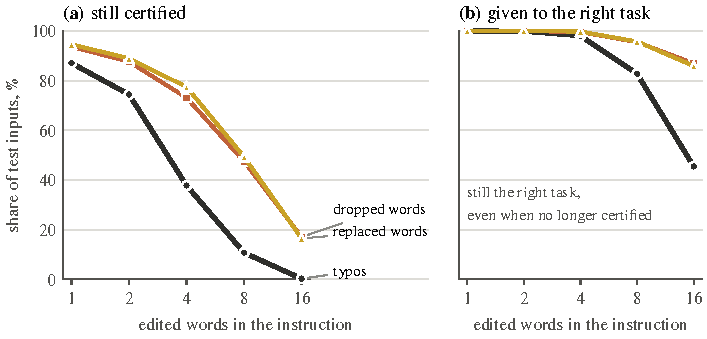
\includegraphics[width=0.86\linewidth]{figures/edits}
  \caption{Mechanical edits of the instruction, all fifteen tasks, routes only (T5-base
  word-vectors; 1{,}197 test inputs per point, each with its own random edit). (a) Share of inputs
  that are still inside their own zone. (b) Share of inputs that are given to their own task.
  No edited input was inside the zone of another task.}
  \label{fig:edits}
\end{figure}

\begin{table}[t]
  \caption{Edits of the whole instruction (same test as Figure~\ref{fig:edits}). Tasks whose
  definition has a single sentence are left out of the last three rows.}
  \label{tab:edits}
  \centering
  \small
  \begin{tabular}{lccccc}
    \toprule
    Edit of the instruction & Tasks & Inputs & Certified inputs, \% & \shortstack[c]{Sent to own\\task, \% $\uparrow$} & Wrong zone \\
    \midrule
    Lower case & 15 & 1197 & 91.4 & 100.0 & 0 \\
    Sentence in front & 15 & 1197 & 91.6 & 100.0 & 0 \\
    First sentence removed & 14 & 1097 & 24.7 & 100.0 & 0 \\
    Last sentence removed & 14 & 1097 & 32.8 & 81.5 & 0 \\
    Sentences shuffled & 14 & 1097 & 100.0 & 100.0 & 0 \\
    \bottomrule
\end{tabular}

\end{table}

\paragraph{No edited input was certified for another task.} Not one of the 23{,}640 edited inputs
lay inside the zone of another task. An edited input was either certified for its own task or not
certified at all. This is a statement about these fifteen tasks, whose instructions are far apart;
in the large collection of Section~\ref{sec:many} the inputs of sibling tasks do lie inside older
zones. A certificate promises that an answer will stay the same, not that it comes from the right
task.

\paragraph{Small edits keep the certificate, large ones lose it.} With one typo 87.1\% of the inputs
are still certified, with one dropped word 93.7\%, with one replaced word 94.6\%, in lower case
91.4\% and with a sentence in front 91.6\% (Figure~\ref{fig:edits}a,
Table~\ref{tab:edits}). With four edited words between 38\% and 77\% remain certified, with sixteen
at most 17\%. A typo costs more than a dropped word, presumably because a misspelt word falls apart into
several rare word pieces, which carry a high weight in Eq.~\eqref{eq:weights}.

\paragraph{The route of an uncertified input is not safe under heavy damage.} Up to four edited
words, at least 98.1\% of the inputs still reach their own task. With eight typos it is 82.7\%, and
with sixteen typos only 45.4\% (Figure~\ref{fig:edits}b). Before the test we had written down that a
share under 80\% for any edit would count against the method, and it does: when an instruction is
badly damaged, the nearest-zone route cannot be relied on. What the method offers in this situation
is the missing certificate, which marks every one of these inputs.

\paragraph{Long instructions are robust, short ones are not.} The failures are not spread evenly
(Table~\ref{tab:editspertask} in the appendix). Tasks whose opening has at least 90 tokens keep
98\% to 100\% of their inputs on the right task even with sixteen typos. The two tasks that fail
first have the shortest instructions: \texttt{sciq}, whose definition has ten words (opening of 26
tokens), and \texttt{xsum} (34 tokens); with eight typos only 3\% and 18\% of their inputs arrive.
With sixteen typos every word of four or more letters in a definition of ten words carries a typo.

\paragraph{Two findings that follow from how the switch reads.} Removing the last sentence of the
definition leaves 81.5\% of the inputs on their task, but only 2\% for SST-2 and 8\% for emotion
classification: in both, the removed sentence is the one that states the task. Shuffling the
sentences changes nothing at all, and every input stays certified, because the feature of
Eq.~\eqref{eq:prefix} is an average and ignores the order of the words
(Proposition~\ref{prop:edits}).

\paragraph{The guaranteed tolerance.} The largest distance between two rows of the rescaled
embedding table of T5-base is $D = 509.6$, and the ratio $R_k / D$ of Proposition~\ref{prop:edits}
lies between 2.0\% and 4.2\% for the fifteen tasks. Edits that remove at most this share of the
weight of the opening, and add at most this share, can therefore never leave the zone. Counted in
tokens of average weight this is the replacement of \BoundTokensLow{} to \BoundTokensHigh{} tokens,
depending on the task. The measured tolerance is far larger, as it should be: the bound has to
cover the two most different tokens of the vocabulary. We also
checked the bound itself on \BoundInputs{} edited inputs of this test (ten per task and edit with
typos, dropped and replaced words). It held for every one of them; the inputs moved by at most
\BoundWorstPct{}\% of what the bound allows, \BoundMedianPct{}\% in the middle, and the bound
alone would have certified \BoundGuaranteed{} of the \BoundInside{} inputs that in fact stayed inside
their zone.


\subsection{The order of the tasks}
\label{sec:orders}

The signature of a task depends on its own opening only, and its radius on the signatures known
when the task arrives. How the routes would look if the tasks had arrived in another order can
therefore be computed exactly, without training. Table~\ref{tab:orders} does this for every one of
the 120 orders of the five tasks, and for the two official orders of the benchmark and 1{,}000 random
orders of the fifteen tasks.

\begin{table}[t]
  \caption{The order of the tasks (routes only, T5-base word-vectors). Entries with four numbers are
  for the original / light / medium / heavy wording; the reworded inputs are those of the five tasks.
  ``Blocked'': training inputs inside an older zone. ``Changed'': test inputs whose route changed
  after their task had been added; where a range is given it depends on the order.}
  \label{tab:orders}
  \centering
  \footnotesize
  \setlength{\tabcolsep}{3.5pt}
  \begin{tabular}{lcccccc}
    \toprule
    Sequence & Orders & \shortstack[c]{Sent to own\\task, \% $\uparrow$} & \shortstack[c]{Certified\\inputs, \%} & Wrong zone & Blocked & \shortstack[c]{Routes\\changed $\downarrow$} \\
    \midrule
    5 tasks, all orders & 120 & 100/100/100/93.8 & 100/100/20/19.6 & 0 & 0 & 0--31 \\
    \midrule
    15 tasks, official order 1 & 1 & 100/100/100/93.8 & 100/100/20/19.6 & 0 & 0 & 0 \\
    15 tasks, official order 2 & 1 & 100/100/100/93.8 & 100/100/20/19.6 & 0 & 0 & 31 \\
    15 tasks, random orders & 1,000 & 100/100/100/93.8 & 100/100/20/19.6 & 0 & 0 & 0--31 \\
    \bottomrule
\end{tabular}

\end{table}

In every order all inputs with the original wording are certified, no input lies in a foreign
zone, no training input is blocked, and the shares of inputs that reach their own task are the
same to the last digit. The reason is plain once the distances are written down
(Table~\ref{tab:distances} in the appendix). For 13 of the 15 tasks the nearest known signature is
that of an unrelated task, and the unrelated tasks are known from the start, so the radius of
these zones does not depend on the order at all. The two exceptions are the summarisation tasks
\texttt{samsum} and \texttt{xsum}, whose nearest signature is a third summarisation task
(\texttt{reddit\_tifu}); their radius is up to 7\% and 13\% smaller if that task was learned
before them, and no test input is affected.

What does depend on the order is \emph{when} an uncertified input goes wrong. The 31 heavily
reworded tweets that are given to SST-2 are given to it from the start if SST-2 is learned before
Sentiment140, as in our five-task sequence and in official order~1. If SST-2 comes later, as in
official order~2, they are first given to their own task and are re-routed at the moment SST-2
arrives. In that order 31 routes change after the inputs were first answered, and with a route the answer
changes in general (this test computes routes only). They are uncertified inputs, and
Proposition~\ref{prop:uncertified} says that this can happen; for certified ones it cannot.


\subsection{The unrelated inputs}
\label{sec:background}

The switch uses the collection $\mathcal{B}$ of unrelated inputs in three places: the token
weights, the scale of distances, and the signatures of the unrelated tasks, which set most radii.
A reader may ask whether the results depend on this particular collection. We repeated the route
computations with two other random draws of the 4{,}000 inputs, with 500, 1{,}000 and 2{,}000 inputs,
and with only five of the ten unrelated tasks, in two ways (Table~\ref{tab:background} in the
appendix; the settings and what would count against the method were again fixed beforehand). In
all eight settings every input with the original or the light wording is certified, every input
with the original, light or medium wording reaches its own task, no input lies in a foreign zone,
and no training input is blocked. The part of the results that rests on the guarantee therefore
did not depend on the choice. The share of heavily reworded inputs that reach their own task did:
it ranges from \BackgroundHeavyLow{}\% to \BackgroundHeavyHigh{}\% across the settings, so the value
of our main configuration, 93.8\%, is one draw from that range and not a property of the method.
One thing we had expected did not happen: with only five unrelated tasks the radii hardly changed (Table~\ref{tab:background}),
and at most two more heavily reworded inputs were certified.


\subsection{Other models}
\label{sec:models}

\paragraph{The routes with other embedding tables.} The switch needs nothing from a model except its
tokenizer and its embedding table, so where the test inputs would be routed can be computed for any
model without training it. Table~\ref{tab:models} does this for eight models of three kinds:
encoder-decoder models (T5 in three sizes \citep{raffel2020t5} and Flan-T5
\citep{chung2024flant5}), decoder-only models (GPT-2 \citep{radford2019gpt2}, SmolLM2
\citep{allal2025smollm2} and Qwen2.5 \citep{yang2024qwen25}) and an encoder (RoBERTa
\citep{liu2019roberta}), with embedding dimensions from 512 to 1024 and five different
vocabularies. Nothing was adjusted per model; the radius factor and the word weights are those of
Section~\ref{sec:method}. For every model, every test input with the original wording lies in its
own zone, in the five-task and in the 15-task sequence, no input lies in a foreign zone, and no
training input of a later task is blocked. With light rewording 99\% to 100\% of the inputs are
certified, and with medium rewording all inputs still reach their own task. Heavy rewording is
where the models differ: between 80\% and 99\% of those inputs reach their own task. Under heavy rewording the routes of three uncertified inputs changed when a later task arrived (two with Flan-T5, one with GPT-2); no certified route changed.

\begin{table}[t]
  \caption{Routes computed with the embedding tables of eight models (CPU, no training). Entries
  with four numbers are for the original / light / medium / heavy wording. ``Wrong zone'': inputs
  inside the zone of another task, over both sequences and all wordings. ``Changed'': inputs
  whose route changed after their task had been added. With the original wording every input of
  the 15-task sequence is certified for every model.}
  \label{tab:models}
  \centering
  \footnotesize
  \setlength{\tabcolsep}{3pt}
  \begin{tabular}{lcccccc}
    \toprule
    & & \multicolumn{2}{c}{Five tasks} & Fifteen tasks & & \\
    \cmidrule(lr){3-4} \cmidrule(lr){5-5}
    Embedding table of & \shortstack[c]{Embedding\\dimension\\$d$} & \shortstack[c]{certified\\inputs, \%} & \shortstack[c]{sent to\\own task,\\\% $\uparrow$} & \shortstack[c]{sent to\\own task,\\\% $\uparrow$} & Wrong zone & \shortstack[c]{Routes\\changed\\$\downarrow$} \\
    \midrule
    \texttt{t5-small} & 512 & 100/100/20/20 & 100/100/100/89 & 100/100/100/89 & 0 & 0 \\
    \texttt{t5-base} & 768 & 100/100/20/20 & 100/100/100/94 & 100/100/100/94 & 0 & 0 \\
    \texttt{t5-large} & 1024 & 100/100/20/19 & 100/100/100/83 & 100/100/100/83 & 0 & 0 \\
    \texttt{flan-t5-base} & 768 & 100/100/20/14 & 100/100/100/99 & 100/100/100/99 & 0 & 2 \\
    \texttt{gpt2} & 768 & 100/99/20/20 & 100/100/100/87 & 100/100/100/87 & 0 & 1 \\
    \texttt{SmolLM2-135M} & 576 & 100/99/20/20 & 100/100/100/82 & 100/100/100/82 & 0 & 0 \\
    \texttt{Qwen2.5-0.5B} & 896 & 100/99/20/20 & 100/100/100/80 & 100/100/100/80 & 0 & 0 \\
    \texttt{roberta-base} & 768 & 100/99/20/20 & 100/100/100/94 & 100/100/100/93 & 0 & 0 \\
    \bottomrule
\end{tabular}

\end{table}

\paragraph{Training other models with the stand-alone code.} To check that the method, and not
only its routes, carries over to other models, we ran the stand-alone implementation
(Appendix~\ref{app:impl}) on three small models on a CPU: T5-small (encoder-decoder), GPT-2 and
SmolLM2-135M (both decoder-only). The runs are small on purpose: the five tasks with 400 training
examples and five epochs each, 30 to 50 test inputs per task, one seed. They show whether the code
keeps answers on another architecture, not how good these models can become. In all three runs
(Table~\ref{tab:demo}) the certified switch ends exactly where it stood right after learning, no
answer of an earlier task changes, and every test input with the original wording is certified. With
all adapters on, the same adapters end at \DemoTfivePlainAP{}, \DemoGptPlainAP{} and
\DemoSmolPlainAP{} instead of \DemoTfiveAP{}, \DemoGptAP{} and \DemoSmolAP{}, and nearly all answers of
earlier tasks change. With heavily reworded instructions no answer changes either, and
\DemoTfiveHeavyRight{}\%, \DemoGptHeavyRight{}\% and \DemoSmolHeavyRight{}\% of those inputs reach
their own task.

\begin{table}[t]
  \caption{The stand-alone implementation on three small models (CPU, five tasks, 400 training
  examples and 5 epochs per task, one seed). ``Changed'': answers of the first four tasks that
  differ at the end. ``Certified'': test inputs with the original wording that are inside a zone.
  ``enc.-dec.'': encoder-decoder; ``dec.-only'': decoder-only.}
  \label{tab:demo}
  \centering
  \footnotesize
  \setlength{\tabcolsep}{3pt}
  \begin{tabular}{llcccccccc}
    \toprule
    & & \multicolumn{3}{c}{\cert{}, original} & \multicolumn{2}{c}{\plain{}, original} & & \multicolumn{2}{c}{\cert{}, heavy} \\
    \cmidrule(lr){3-5} \cmidrule(lr){6-7} \cmidrule(lr){9-10}
    Model & Kind & \shortstack[c]{Score\\right\\after\\learning\\$\uparrow$} & \shortstack[c]{Final\\score\\$\uparrow$} & \shortstack[c]{Answers\\changed $\downarrow$} & \shortstack[c]{Final\\score\\$\uparrow$} & \shortstack[c]{Answers\\changed $\downarrow$} & \shortstack[c]{Certified\\inputs} & \shortstack[c]{Final\\score\\$\uparrow$} & \shortstack[c]{Answers\\changed $\downarrow$} \\
    \midrule
    \texttt{SmolLM2-135M} & dec.-only & 74.3 & 74.3 & 0 of 120 & 27.7 & 100 of 120 & 150 of 150 & 65.1 & 0 of 120 \\
    \texttt{gpt2} & dec.-only & 67.9 & 67.9 & 0 of 120 & 15.8 & 119 of 120 & 150 of 150 & 54.8 & 0 of 120 \\
    \texttt{t5-small} & enc.-dec. & 65.8 & 65.8 & 0 of 200 & 12.0 & 200 of 200 & 250 of 250 & 56.2 & 0 of 200 \\
    \bottomrule
\end{tabular}

\end{table}

\paragraph{A sibling task, with trained answers.} The variant \exactfirst{} was also run with the
stand-alone code on T5-small. After the five tasks a sixth task is learned: the sentences of SST-2
under the lightly reworded definition of SST-2, but with other answer words (``good'' and ``bad''
instead of ``POS'' and ``NEG''), so that one can see which adapters answered. The sixth task is
learned twice from the same starting point. Under \cert{}, all \SiblingCertBlocked{} of its
\SiblingTrain{} training inputs are blocked; after training, its test inputs are still answered in
the words of the old task (\SiblingCertRight{} of \SiblingTest{} right), and no answer of the five
old tasks changes in any wording. Under \exactfirst{} the task is learned (\SiblingExactRight{} of
\SiblingTest{} right), no answer to an unedited input of the old tasks changes, and the
\SiblingExactChangedLight{} old test inputs of SST-2 that carry the sibling's instruction word for
word now get the sibling's answer; nothing else changes (\SiblingOldInputs{} old test inputs per
wording). This is one small model and one constructed sibling. It shows the two behaviours side by side with trained answers, and it is not a test of the variant at scale.


\subsection{Rewording at scale: machine paraphrases of 700 real tasks}
\label{sec:paraphrase}

Our other tests of rewording rest on the development rewordings (five tasks) or on
damage made by a program (Section~\ref{sec:edits}). Here the rewordings come from neither. We took
the \WidenTasksAll{} definitions of Section~\ref{sec:many} and paraphrased each one by machine: back-translation
from English into German and back, and into French and back, sentence by sentence, with MarianMT
models \citep{junczys2018marian,tiedemann2020opusmt} and beam search without sampling. On average
\WidenKeptDe{}\% (German) and \WidenKeptFr{}\% (French) of the words of a definition survive; \WidenSameDe{}
German and \WidenSameFr{} French paraphrases equal the original. Two more pivots, Spanish and Italian, were made later, for the checks below (\WidenSpKept{}\% and \RerouteItKept{}\% of the words survive; \WidenSpSame{} and \RerouteItSame{} paraphrases equal the original). Two more pivots, Spanish and Italian, were made later, for the checks below (\WidenSpKept{}\% and \RerouteItKept{}\% of the words survive; \WidenSpSame{} and \RerouteItSame{} paraphrases equal the original). They are used as they come, poor
ones included. A paraphrased input is an input of its task whose definition has been replaced by the
paraphrase. \WidenTasksCal{} of the tasks are kept for choosing and calibrating (they are not used
again), and \WidenTasksEval{} are used for evaluation, arriving in a random order, each with its
zone. No model is trained; the test is about routes, with the T5-base word-vectors and the rule of
Section~\ref{sec:method} unchanged.

\paragraph{Measures.} All are shares. \textsf{C}: tasks that arrive with at least one unedited input inside an
older zone. \textsf{U}: unedited inputs given to their own task. \textsf{P}: paraphrased inputs that lie inside their
own task's zone and are given to it, a correct certificate. \textsf{M}: paraphrased inputs that are certified
for \emph{another} task, a wrong certificate: the answer is stable, but it comes from the wrong
adapters. \textsf{R}: paraphrased inputs given to their own task, with or without a certificate. These letters name measures in this section and its appendix only; they are not the covariance, the radius or the zone of the method.

\paragraph{The result for \cert{}.} With \WidenParaInputs{} paraphrased inputs (German and
French pivot together) we find \textsf{C}~=~\WidenRefTfiveC{}\%, \textsf{U}~=~\WidenRefTfiveU{}\%, \textsf{P}~=~\WidenRefTfiveP{}\%,
\textsf{M}~=~\WidenRefTfiveM{}\% and \textsf{R}~=~\WidenRefTfiveR{}\%. By pivot, \textsf{P} is \WidenRefTfiveFrP{}\% (French),
\WidenRefTfiveDeP{}\% (German) and \WidenRefTfiveEsP{}\% (Spanish); \textsf{M} is \WidenRefTfiveFrM{}\%,
\WidenRefTfiveDeM{}\% and \WidenRefTfiveEsM{}\%; \textsf{R} is \WidenRefTfiveFrR{}\%, \WidenRefTfiveDeR{}\% and
\WidenRefTfiveEsR{}\%. The Spanish paraphrases were made later, for the check described below, and the Italian ones last, for the fallback tests (on the Italian pivot \textsf{P}~=~\WidenRefTfiveItP{}\%, \textsf{M}~=~\WidenRefTfiveItM{}\%,
\textsf{R}~=~\WidenRefTfiveItR{}\%, inside the same ranges); \cert{} was not tuned on any of the four. So between four and five in ten machine-paraphrased inputs get a correct certificate
(\WidenRefTfivePLow{}\% to \WidenRefTfivePHigh{}\%, depending on the language the paraphrase went through), \WidenRefTfiveMLow{}\% to
\WidenRefTfiveMHigh{}\% are certified for another task, and the rest are uncertified. About three quarters of all paraphrased inputs (\WidenRefTfiveRLow{}\% to \WidenRefTfiveRHigh{}\%) reach their own task, with or
without a certificate. The figures of \FiveCertRightLight{}\%, \FiveCertRightMedium{}\% and
\FiveCertRightHeavy{}\% of Section~\ref{sec:reworded} were measured on five tasks that are far apart and on the development
rewordings. This is a limitation of the method as built: the zones are narrow at scale.

\paragraph{Can the zones be made wider?} We tried five ways, each with a rule for success written
before the run (Appendix~\ref{app:widen}): (1) the hidden states of a frozen causal language model
instead of the word-vectors; (2) a metric that counts distance in units of what paraphrasing does;
(3) a frozen sentence encoder of 22 million weights \citep{reimers2019sbert,wang2020minilm} with
a radius set by split-conformal calibration; (4) a zone decided by a frozen inference model
\citep{he2023debertav3} that judges whether two instructions ask for the same thing; (5) the same kind of judge, asked sentence by sentence. None of the five met the bar set for it in advance
(Table~\ref{tab:widenmain}, Figure~\ref{fig:widen}). For (3) to (5) the bar was \textsf{P}~$\ge$~75\%, \textsf{M}~$\le$~5\% and \textsf{C}~$\le$~19\%, read on the French pivot for (3) and (4) and on the Italian pivot for (5); the encoder reached \textsf{P}~=~\WidenEncPrimP{}\%,
\textsf{M}~=~\WidenEncPrimM{}\% and \textsf{C}~=~\WidenEncPrimC{}\%, the judge \textsf{P}~=~\WidenJudgeFrP{}\%,
\textsf{M}~=~\WidenJudgeFrM{}\% and \textsf{C}~=~\WidenJudgeC{}\%; (5) reached, on the Italian pivot that no study had read, \textsf{P}~=~\WidenSentItP{}\%, \textsf{M}~=~\WidenSentItM{}\% and \textsf{C}~=~\WidenSentC{}\%, the best point so far: \textsf{P} and \textsf{C} are on the right side of the success lines, \textsf{M} is above the 9\% limit.

\begin{table}[t]
  \caption{Machine paraphrases of 700 real tasks, routes only: \cert{} and the
  attempts to widen the zones, each in the setting named before its run. \textsf{C}: tasks that collide;
  \textsf{P}: paraphrased inputs certified for their own task; \textsf{M}: certified for another task; \textsf{R}: given to
  their own task; all in \%. ``Both'': German and French pivot together. Paper: T5-base word-vectors, weighted mean,
  $\kappa = 0.5$; its second row is the French pivot alone, the reference for the rows (2) to (4), which are French. (1) was run with another model, SmolLM2-135M, so it has its own reference row; the
  hidden state is that of the last layer, with one radius for all tasks. (2) uses the T5-base word-vectors with a metric fitted on
  paraphrases, read at the radius where \textsf{C} equals that of \cert{}, which is why its \textsf{C} is the same.
  (3) is MiniLM-L6 with the paraphrase ruler and a split-conformal radius ($\alpha = 0.1$); (4) is a MiniLM filter and the
  DeBERTa-v3-xsmall inference model ($\tau = \WidenJudgeTau{}$); (5) the same judge, sentence by sentence, read on the Italian pivot (its French-pivot point is in Figure~\ref{fig:widen}). Settings other than these are in
  Appendix~\ref{app:widen}. Units: rows marked ``both'' use \WidenParaInputs{} paraphrased inputs, the French rows \WidenParaInputsPivot{}, except (4) and (5), which
  take the instruction as a separate field and count one paraphrased instruction per task (\WidenTasksEval{}); its \textsf{C} is about the tasks' original
  instructions. The pre-registered reference of (2) is the old ruler at the same radius (\textsf{P} \WidenRulerTfivePOld{}\%, \textsf{M} \WidenRulerTfiveMOld{}\%).}
  \label{tab:widenmain}
  \centering
  \footnotesize
  \setlength{\tabcolsep}{3pt}
  \begin{tabular}{llcrrrrl}
    \toprule
    & Features and zone & Pivot & \textsf{C} & \textsf{P} & \textsf{M} & \textsf{R} & Verdict \\
    \midrule
    Paper & T5-base word-vectors, weighted mean & both & 16.9 & 40.5 & 7.6 & 75.4 & reference \\
    Paper & T5-base word-vectors, weighted mean & French & 16.9 & 39.8 & 9.2 & 75.4 & ref. for (2)--(4) \\
    \midrule
    (1) & SmolLM2 word-vectors & both & 18.9 & 42.1 & 8.9 & 75.6 & ref. for (1) \\
    (1) & SmolLM2 last layer & both & 25.7 & 64.9 & 13.7 & 83.2 & against \\
    (2) & T5-base, paraphrase ruler & French & 16.9 & 42.0 & 10.7 & 84.4 & against \\
    (3) & MiniLM, ruler, $\alpha = 0.1$ & French & 16.6 & 71.2 & 11.6 & 86.1 & against \\
    (4) & MiniLM and NLI judge & French & 36.0 & 58.9 & 34.7 & 64.7 & against \\
    (5) & MiniLM, sentence-wise NLI judge & Italian & 12.4 & 76.1 & 10.9 & 88.7 & against \\
    \midrule
    Bar (3)--(5) & \multicolumn{2}{l}{fixed in advance} & $\le 19$ & $\ge 75$ & $\le 5$ & & \\
    \bottomrule
\end{tabular}

\end{table}

\begin{figure}[t]
  \centering
  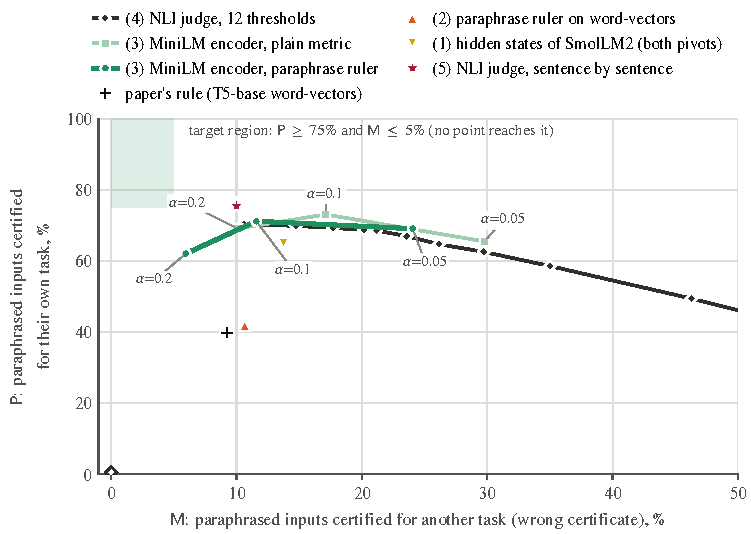
\includegraphics[width=0.86\linewidth]{figures/widen_tradeoff}
  \caption{Correct against wrong certificates on paraphrased inputs (French pivot; hidden states of
  (1): both pivots). The shaded box is the target. The sentence encoder (3) is shown plain and with
  the paraphrase ruler at $\alpha = 0.05, 0.1, 0.2$; the curve of the judge (4) has one point per
  threshold, and its point at the strictest threshold (open) covers almost nothing. One point
  of the curve (the loosest threshold) lies beyond the right edge. Only (3) at $\alpha = 0.1$ with the ruler, (4) at $\tau = \WidenJudgeTau{}$ and (5) were named before the runs; (5) is shown at its French-pivot value.}
  \label{fig:widen}
\end{figure}

\paragraph{What rises and what does not.} The sentence encoder lifts the share of correct certificates
from \WidenRefTfiveFrP{}\% (\cert{}, French pivot alone) to between \WidenEncRulerTwentyFrP{}\% and
\WidenEncPlainTenFrP{}\% over its six settings (Table~\ref{tab:widenencoder} in the appendix). At $\alpha = 0.1$ and
$0.2$ ($\alpha$ is the level of the split-conformal radius, not the scaling factor of the adapters) it gives between \WidenEncRHighLow{}\% and \WidenEncRHighHigh{}\% of the inputs to the right task, where \cert{}
gives \WidenRefTfiveFrR{}\%. The wrong certificates do not stay low as \textsf{P} rises. The setting with the fewest
(\textsf{M}~=~\WidenEncRulerTwentyFrM{}\%, above the bar of 5\%) has \textsf{P}~=~\WidenEncRulerTwentyFrP{}\%, and the setting with the
highest \textsf{P} (\WidenEncPlainTenFrP{}\%) has \textsf{M}~=~\WidenEncPlainTenFrM{}\%. \cert{} has \textsf{M}~=~\WidenRefTfiveFrM{}\%
on the French pivot alone, so the first setting is lower in \textsf{M} and higher in \textsf{P} than \cert{}; it was
not the primary setting, and we checked it on held-out paraphrases (next paragraph). Most of the tasks that collide under \cert{} are siblings
that differ in one or a few decisive words: a date format day-month against month-day, the closest integers against
the farthest, the reaction of a person in the ATOMIC tasks against their intent
(Table~\ref{tab:widensiblings} in the appendix, a selection). Every feature for which we inspected the collisions puts the
rewordings of such siblings together. The judge also certifies some paraphrases for unrelated tasks, for example
sentence generation from a relation for an entailment task. The judge is good on single pairs (area under the curve
\WidenJudgeAucNli{} on calibration pairs) and bad as a zone: a text is judged against up to \WidenJudgeLimit{} nearby
instructions, and one wrong ``same'' from an older zone, or from any zone when its own zone does not hold it, is enough.

\paragraph{One setting, checked on held-out paraphrases.} After the runs we saw that one setting of the sentence
encoder that was not the primary one (paraphrase ruler, $\alpha = 0.2$) was ahead of \cert{} on the French pivot
on each measure. A comparison chosen after the results proves nothing, so we fixed one more check before running it: the same two
rules on paraphrases made through Spanish, which no study had read, on the same \WidenTasksEval{} tasks, with nothing fitted again.
It would count as confirmed if the encoder setting gained at least \WidenSpAskP{} points in \textsf{P} and \WidenSpAskR{} points in \textsf{R}
and had no more wrong certificates. On the Spanish pivot (Table~\ref{tab:widenspanish}) \cert{} has
\textsf{P}~=~\WidenRefTfiveEsP{}\%, \textsf{M}~=~\WidenRefTfiveEsM{}\% and \textsf{R}~=~\WidenRefTfiveEsR{}\%, the encoder setting \textsf{P}~=~\WidenSpEncEsP{}\%,
\textsf{M}~=~\WidenSpEncEsM{}\% and \textsf{R}~=~\WidenSpEncEsR{}\%. The gain in \textsf{P} is \WidenSpGainP{} points, so by our rule the check is \emph{not
confirmed} (the gain in \textsf{R}, \WidenSpGainR{} points, and \textsf{M} pass). On this split the encoder setting is ahead on each measure, but by less than we
asked for; \cert{} itself does better on these paraphrases, which keep more of the original words
(\WidenSpKept{}\% against \WidenKeptDe{}\% and \WidenKeptFr{}\%). On \WidenSplitCount{} other random splits of the tasks into calibration and
evaluation tasks (everything fitted again), the Spanish pivot gives \textsf{P} of \WidenSplitRulePMean{}\% (\WidenSplitRulePLow{} to
\WidenSplitRulePHigh{}) and \textsf{M} of \WidenSplitRuleMMean{}\% (\WidenSplitRuleMLow{} to \WidenSplitRuleMHigh{}) for \cert{}, and
\textsf{P} of \WidenSplitEncPMean{}\% (\WidenSplitEncPLow{} to \WidenSplitEncPHigh{}) and \textsf{M} of \WidenSplitEncMMean{}\%
(\WidenSplitEncMLow{} to \WidenSplitEncMHigh{}) for the encoder setting, which therefore depends more on the split. On \WidenSplitMoreM{} of these \WidenSplitCount{} splits the encoder setting has more wrong
certificates than \cert{} (and on \WidenSplitMoreC{} of them more collisions), so the advantage on every measure is a property
of the original split, not of the setting. We report the encoder
zone as a variant, not as an improvement that we have shown. It needs a second model, run at several prefix lengths, for every input
(\WidenEncMs{} ms per input on two CPU threads), it has no edit bound, its radius does not keep the promised coverage on another pivot (\textsf{Z} is
\WidenSpEncEsZ{}\% on Spanish and \WidenSpEncFrZ{}\% on French where \WidenSpPromise{}\% was promised, and \WidenSpEncDeZ{}\% on the German pivot it
was fitted on), and with it none of the medium and heavy development rewordings of the five benchmark tasks lies inside a zone
(\WidenSpBenchMediumZone{}\% and \WidenSpBenchHeavyZone{}\%); they are still given to the right task.

\begin{table}[t]
  \caption{The check on Spanish-pivot paraphrases: \cert{} and the encoder setting (paraphrase ruler,
  $\alpha = 0.2$) on the three pivots, \WidenSpInputs{} paraphrased inputs each; nothing was fitted again for Spanish. ``Encoder'': the sentence encoder with the paraphrase ruler at $\alpha = 0.2$. In \%.}
  \label{tab:widenspanish}
  \centering
  \footnotesize
  \setlength{\tabcolsep}{3pt}
  \begin{tabular}{lrrrrrrrrrr}
    \toprule
    & & \multicolumn{3}{c}{French} & \multicolumn{3}{c}{German} & \multicolumn{3}{c}{Spanish} \\
    \cmidrule(lr){3-5} \cmidrule(lr){6-8} \cmidrule(lr){9-11}
    & \textsf{C} & \textsf{P} & \textsf{M} & \textsf{R} & \textsf{P} & \textsf{M} & \textsf{R} & \textsf{P} & \textsf{M} & \textsf{R} \\
    \midrule
    Paper's rule & 16.9 & 39.8 & 9.2 & 75.4 & 41.2 & 5.9 & 75.5 & 50.4 & 9.7 & 77.5 \\
    Encoder & 12.1 & 62.1 & 6.0 & 90.0 & 72.6 & 8.1 & 89.7 & 63.8 & 5.3 & 91.7 \\
    \bottomrule
\end{tabular}

\end{table}

\begin{table}[t]
  \caption{The same two rules on \WidenSplitCount{} other random splits of the \WidenTasksAll{} tasks, Spanish pivot: mean (smallest to largest), with
  ruler and radius fitted again on each split. In \%.}
  \label{tab:widensplits}
  \centering
  \footnotesize
  \begin{tabular}{lcc}
    \toprule
    Spanish pivot & Paper's rule & Encoder \\
    \midrule
    Tasks that collide (\textsf{C}), \% $\downarrow$ & 16.0 (14.3 to 17.3) & 12.7 (9.1 to 16.6) \\
    Right certificate (\textsf{P}), \% $\uparrow$ & 49.4 (48.3 to 50.7) & 63.1 (55.5 to 70.0) \\
    Wrong certificate (\textsf{M}), \% $\downarrow$ & 7.9 (4.2 to 10.4) & 6.0 (2.4 to 9.7) \\
    Sent to own task (\textsf{R}), \% $\uparrow$ & 76.9 (75.8 to 78.1) & 90.4 (87.7 to 93.3) \\
    \bottomrule
\end{tabular}

\end{table}

\paragraph{Do later tasks re-route reworded inputs?} The stress test of Section~\ref{sec:stress} built by hand a case in which a best-match rule
changes an old route. With the paraphrased inputs we can count how often this happens among real tasks. For every paraphrased input we compare its route
right after its own task has arrived with its route after all \WidenTasksEval{} tasks. The reading was fixed before the run (Appendix~\ref{app:reroute}): the zones
add something at scale if \nearest{} changes at least 5\% of the routes and \cert{} at most half as many, and little if \nearest{} changes fewer than \RerouteLimitLow{}\%.

The result is against us (Table~\ref{tab:reroute}); by the reading fixed in advance, ``the zones add little here''. \nearest{} changed \RerouteNearNChanged{} of \RerouteInputs{} routes (\RerouteNearChanged{}\%), and \cert{} changed the same
\RerouteCertNChanged{}, all of them outside every zone. None of the \RerouteCertInZone{}\% of the inputs that were inside a zone at arrival changed, as Theorem~\ref{thm:writeonce} says, but
the nearest-zone rule did not change them either. We had expected \RerouteExpectNearLow{}\% to \RerouteExpectNearHigh{}\% for \nearest{}; that expectation was wrong. In this collection the certified switch adds
the proof, and no stability that we could measure.

\begin{table}[t]
  \caption{Do later tasks re-route reworded inputs? Routes only; \WidenTasksEval{} real tasks. ``Own'': share of the \RerouteInputs{} paraphrased inputs (French and German pivot) given to their own task after all tasks; ``Italian: own'':
  the same on the \RerouteInputsPivot{} Italian-pivot inputs (paraphrases made for the two fallback tests and read only for them). ``Changed'': route after all tasks differs from the route right after the input's own task arrived. ``In a zone'': inside a zone
  at arrival. ``Unedited'': unedited inputs given to their own task at the end (none changed under any rule). \signature{}: nearest signature in plain distance, no radius. \hybrid{}: the oldest zone that holds the
  input, else the nearest signature in plain distance. \scaled{}: nearest signature, its distance divided by the distance of the task's signature to the nearest signature of the unrelated tasks. \certscaled{}: the oldest zone that holds the input, else \scaled{}.
  \hybrid{} was designed after the first three results were seen and \scaled{} after \hybrid{}, on the same data; none has a free setting.}
  \label{tab:reroute}
  \centering
  \scriptsize
  \setlength{\tabcolsep}{2pt}
  \begin{tabular}{lrrrrr}
    \toprule
    Rule & \shortstack[r]{Sent to own\\task, \% $\uparrow$} & \shortstack[r]{Italian pivot: sent\\to own task, \% $\uparrow$} & \shortstack[r]{Routes changed,\\\% (n) $\downarrow$} & \shortstack[r]{Inside a zone\\at arrival, \%} & \shortstack[r]{Unedited, sent to\\own task, \% $\uparrow$} \\
    \midrule
    \signature{} (plain nearest signature) & 91.3 & 93.1 & 2.22 (93) & -- & 98.4 \\
    \nearest{} (nearest zone) & 75.4 & 77.0 & 0.31 (13) & -- & 98.4 \\
    \cert{} (the rule of the paper) & 75.4 & 76.8 & 0.31 (13) & 48.1 & 83.1 \\
    \hybrid{} (zones, then nearest signature) & 85.6 & 88.5 & 1.95 (82) & 48.1 & 83.1 \\
    \scaled{} (scaled by the distance to unrelated text) & 94.4 & 95.9 & 1.60 (67) & -- & 98.4 \\
    \certscaled{} (zones, then \scaled{}) & 88.6 & 91.3 & 1.33 (56) & 48.1 & 83.1 \\
    \bottomrule
\end{tabular}

\end{table}

\begin{table}[t]
  \caption{The same rules on the benchmark tasks with the development rewordings (routes only): share of the \RerouteBenchInputs{} inputs given to their own task after the last task; ``(n)'': routes changed by later tasks (of \RerouteBenchInputs{}, including the inputs of the last task, which cannot change).
  With the original and the light wording every rule gives 100\% and changes nothing.}
  \label{tab:reroutebench}
  \centering
  \footnotesize
  \setlength{\tabcolsep}{3pt}
  \begin{tabular}{lrrrr}
    \toprule
    & \multicolumn{2}{c}{Five tasks} & \multicolumn{2}{c}{Fifteen tasks} \\
    \cmidrule(lr){2-3} \cmidrule(lr){4-5}
    Rule & \shortstack[r]{Medium wording:\\own task, \% $\uparrow$\\(routes changed)} & \shortstack[r]{Heavy wording:\\own task, \% $\uparrow$\\(routes changed)} & \shortstack[r]{Medium wording:\\own task, \% $\uparrow$\\(routes changed)} & \shortstack[r]{Heavy wording:\\own task, \% $\uparrow$\\(routes changed)} \\
    \midrule
    \signature{} & 76.8 (55) & 60.0 (100) & 71.6 (74) & 60.0 (100) \\
    \nearest{} & 100.0 (0) & 93.8 (0) & 100.0 (0) & 93.8 (0) \\
    \cert{} & 100.0 (0) & 93.8 (0) & 100.0 (0) & 93.8 (0) \\
    \hybrid{} & 76.8 (55) & 60.0 (100) & 71.6 (74) & 60.0 (100) \\
    \scaled{} & 100.0 (0) & 93.8 (0) & 100.0 (0) & 93.8 (0) \\
    \certscaled{} & 100.0 (0) & 93.8 (0) & 100.0 (0) & 93.8 (0) \\
    \bottomrule
\end{tabular}

\end{table}

Two more rules were computed on the same routes after this result, each written down before it was computed. The plain nearest signature, without radii, is the usual prototype rule. It changed
\RerouteSigNChanged{} routes (\RerouteSigChanged{}\%), and \RerouteSigNLost{} inputs lost their own task; by its reading fixed in advance that is ``some'' re-routing, less than the 5\% we had expected.
But it gave \RerouteSigOwnEnd{}\% of the paraphrased inputs to their own task, where \cert{} and \nearest{} give \RerouteCertOwnEnd{}\% (Spanish pivot: \RerouteSigEsOwn{}\% against \RerouteCertEsOwn{}\% for \cert{} and \RerouteNearEsOwn{}\% for \nearest{}; unedited inputs:
\RerouteSigUnOwn{}\% against \RerouteCertUnOwn{}\%). At this scale the simplest rule serves reworded inputs better than \cert{}, and it pays with about two silent changes in a hundred inputs. Dividing the distance by the radius is the fallback that
we chose on the benchmark tasks; it keeps routes stable here and gives fewer inputs to their own task.

Zones first and the plain nearest signature outside them (\hybrid{}, designed after the result of the plain nearest signature was seen, on the same data, with no free setting) keeps every certificate and gives \RerouteHybOwnEnd{}\% of the inputs to their own task, with \RerouteHybChanged{}\% changed routes. It is not a repair. On the benchmark tasks with
the development rewordings the plain fallback is much worse than the fallback of \cert{}: \RerouteHybBenchFiveHeavyOwn{}\% against \RerouteCertBenchFiveHeavyOwn{}\% under the heavy rewording, and \RerouteHybBenchFiveHeavyChanged{} of the \RerouteBenchChangeable{} routes
that later tasks could change are changed by them. The two fallbacks trade places between the two tests.

A reading of why, from the numbers and not a test of its own: the radius of a zone is half the distance to the nearest known signature, and ``known'' means the unrelated tasks \emph{and} the earlier tasks. Write $U_k$ for the distance from the signature of task $k$ to the nearest
signature of the unrelated tasks only. On the benchmark tasks the radius is half of $U_k$ for all five tasks and for \RerouteBBenchFifteenCount{} of the fifteen; among the \WidenTasksEval{} real tasks it is so for only \RerouteBShare{}\% of them. For the others an earlier task, usually a
sibling, is nearer than every unrelated one; the radius of the newer sibling is then tiny, and its reworded inputs look far from it and are turned away by the nearest-zone fallback.

We then tested two fallbacks, each with its rule fixed before the run and with the verdict at scale read on paraphrases through a fourth language, Italian, that no study had read (Appendix~\ref{app:reroute}). Success meant at least \RerouteLineHeavy{}\% of the inputs to their own task under
heavy and \RerouteLineMedium{}\% under medium rewording on the benchmark tasks (five and fifteen), and at least \RerouteLineItalian{}\% on the Italian pivot; heavy rewording below \RerouteLineHeavyAgainst{}\% or the Italian pivot below \RerouteLineItalianAgainst{}\% counted against. A fallback scaled by the length of the opening
\emph{failed}: \RerouteNormHeavyFive{}\% under heavy rewording on the benchmark, although it gave \RerouteNormItOwn{}\% on the Italian pivot. A fallback scaled by $U_k$ alone, \scaled{}, \emph{succeeded} (Tables~\ref{tab:reroute} and~\ref{tab:reroutebench}): \RerouteBgHeavyFive{}\% under heavy and \RerouteBgMediumFive{}\% under medium rewording on the benchmark, as
the fallback of \cert{}, and \RerouteBgItOwn{}\% of the Italian-pivot inputs to their own task (plain nearest signature \RerouteSigItOwn{}\%, nearest zone \RerouteNearItOwn{}\%), \RerouteBgOwnEnd{}\% on the French and German pivot. With the zones of \cert{} in front (\certscaled{}: the same zones, the same certificates, the same theorem) it gives
\RerouteCertFourItOwn{}\% on the Italian pivot and \RerouteCertFourOwnEnd{}\% on the French and German pivot, where \cert{} gives \RerouteCertItOwn{}\% and \RerouteCertOwnEnd{}\%, and on the benchmark the routes and shares are those of \cert{}.

It has costs. After their task has arrived \RerouteCertFourChanged{}\% to \RerouteBgChanged{}\% of the paraphrased inputs change their route (French and German pivot; \RerouteBgItChanged{}\% on the Italian and \RerouteCertFourEsChanged{}\% to \RerouteBgEsChanged{}\% on the Spanish pivot; \RerouteCertChanged{}\% with the fallback of \cert{}). In the stress test of Section~\ref{sec:stress} a look-alike task takes uncertified old inputs that the fallback of \cert{} kept: with the light rewording as its definition \RerouteStressCertFourMedium{} of \RerouteStressOld{} with the medium and \RerouteStressCertFourHeavy{} with the heavy wording (0 and 0 for the fallback of \cert{}), and with the medium rewording as its definition \RerouteStressMedCertFourHeavy{} of \RerouteStressOld{} with the heavy wording (\RerouteStressMedCertHeavy{} for the fallback of \cert{}); no certified input changes. Its status: a variant found at the end of this work. The benchmark rewordings are the development set, so on that side it is no independent test;
no GPU run was repeated with it, but an input-by-input check on the benchmark sequences found its routes identical to those of \cert{} at every point where a score is taken. For the five-task sequence the radius is half of $U_k$ for all five tasks, so the two fallbacks order the tasks identically and the routes are the same by construction (the check finds \RerouteIdFiveLast{} differing routes in \RerouteIdFiveComparisons{} comparisons). For the fifteen-task sequence one task, \texttt{\RerouteIdTask{}} (the \RerouteIdTaskPos{}rd to arrive), has a radius that is half the distance to an earlier task and not half of $U_k$; even so \RerouteIdFifteenLast{} routes differ after the last task and \RerouteIdFifteenScored{} at any point from the arrival of the input's own task on, in every wording (they differ only at points before the input's own task has arrived, where no score is taken: \RerouteIdFifteenBeforeOriginal{}, \RerouteIdFifteenBeforeMedium{} and \RerouteIdFifteenBeforeHeavy{} inputs with the original, medium and heavy wording). Every score of the GPU runs of \cert{} and \nearest{} in this paper, for five and for fifteen tasks, is therefore also the score of the corresponding variant. The other route tests were not repeated with it (except the stress test), \cert{} remains the zone rule of every GPU run with instructions, and the certificates are the same under both. With this fallback the zones cost \RerouteZonesCost{} points of right routes on the Italian pivot, \RerouteZonesCostFG{} on the French and German pivot and \RerouteZonesCostEs{} on the Spanish pivot
compared with the best rule without zones (\RerouteBgItOwn{}\% against \RerouteCertFourItOwn{}\%, \RerouteBgOwnEnd{}\% against \RerouteCertFourOwnEnd{}\%), and give a proof for about half of the inputs (\RerouteCertInZone{}\% at arrival). None of these rules was run with trained answers.

\paragraph{The guarantee does not depend on the zone.} Theorem~\ref{thm:writeonce} needs only that the
zone of a task is a fixed set once the task has arrived and that membership is computed reproducibly from frozen parts
(Remark~\ref{rem:otherzones}); the proof does not use how the set was built. It therefore holds for every zone in this
section as defined; for the judge zone as measured, which judges only the \WidenJudgeLimit{} nearest tasks, see Appendix~\ref{app:widen}. What changes is how many inputs a zone covers, and for which task: a certificate promises a
stable answer, not the right task, and a certificate for the wrong task is a stable wrong routing.
The edit bound of Proposition~\ref{prop:edits} does not carry over, because it needs an average.

\paragraph{What this test is not.} Machine paraphrases are made by translation models, not by people.
There is one collection of tasks, in which many tasks are siblings, and the calibration and the
evaluation tasks come from it; the test uses one split and one order of arrival, except for the \WidenSplitCount{} extra splits of the Spanish check. The development rewordings of the five benchmark tasks
move further than a back-translation does: with the sentence encoder
\WidenEncBenchMediumZone{}\% (medium) and \WidenEncBenchHeavyZone{}\% (heavy) of them lie inside their own
zone, while all are still given to the right task. The settings that were not the primary ones
are observations made after the run, and none of them meets the bar.


\subsection{Zones from the inputs of a task: the first test without instructions}
\label{sec:noinstruction}

This subsection reports the first test of the rule of Section~\ref{sec:bound}: a version of the zones that needs no instruction, with a guarantee on how much can be forgotten. It was run before the recogniser of Section~\ref{sec:recogniser} existed, and what it found is the reason why that recogniser was built; the reader has met the recogniser first, and here the story goes back to this earlier step.
The rule and its guarantee are Theorem~\ref{thm:bound} (Section~\ref{sec:bound}): a zone is built from the inputs of the task itself, its size is set on inputs of the task that were held out, and then, for any model and any later tasks, each input of the task changes its answer with probability at most a chosen level.
The test below is a first, small check of that statement on benchmark files. It is routes only, on a CPU: no model was trained and no GPU was used, so it says nothing yet about answers.

\paragraph{Set-up (fixed in the plan of the repository before the run).} We use the official benchmark files, the instances only; the definition of a task is never read. Three sequences: the 15 tasks of SuperNI order~1 of Section~\ref{sec:protocol}, the 15 tasks of the Long Sequence benchmark in its
official order~3, and the two together as one sequence of \BoundTasksBoth{} tasks. All the training inputs of a task are used for its zone (the plan said 800; the largest file, of the Long Sequence benchmark, has \BoundTrainMax{}), and the official test inputs, which are never used for a zone, for the measures; so the condition of the theorem, that the test inputs are like the training inputs, is assumed here for the benchmark's own split; the coverage line below checks it.
The frozen feature of an input is the weighted, rescaled average of the T5-base word-vectors of all its tokens (cut at 256 tokens), as in the rule \centre{} (its token weights and rescaling use the dev files of ten of the Long Sequence tasks, frozen, not their training or test data). The score $a_k(x)$ of the primary setting is the distance of the feature to its 10th nearest neighbour among the fit inputs of task $k$; a second score, reported next to it, is the distance to the mean of the fit features. A third score, designed later, is described below. When task $k$ arrives,
\BoundMCal{} of its training inputs are held out for calibration (for the \BoundSmallTasks{} tasks with fewer than 400 training inputs, half of them, a deviation from the plan forced by the data; the smallest file has \BoundSmallMin{}), the level is $\beta = 0.05$ (levels 0.1 and 0.2 are reported), and $q_k$ is the split-conformal quantile of Section~\ref{sec:bound}. An input goes to the oldest zone that holds it; an input outside every zone goes to the task with the smallest score divided by its $q_k$.
Four measures, per task and averaged over the tasks of a sequence: the share of its test inputs inside its own zone (covered); the share inside the zone of an older task when the task arrives (blocked); the share given to the own task after the last task (own task); the share whose route after the last task differs from the route when their task arrived (changed).

\paragraph{Two lines, fixed before the run.} (1) \emph{The claim:} on each sequence the average share of changed routes must be at most $\beta$ plus two standard errors and the average coverage at least $1 - \beta$ minus two standard errors; if not, the assumption that test inputs are like training inputs fails on these files, and the paper has to say so. (2) \emph{The use:} ``works without instructions'' on a sequence if on average at least \BoundLineOwn{}\% of the test inputs go to their own task and at most \BoundLineBlock{}\% are blocked; ``does not'' if fewer than \BoundLineNotOwn{}\% go to their own task or more than \BoundLineNotBlock{}\% are blocked; otherwise partial.

\begin{table}[t]
  \caption{Zones from the inputs of a task, no instruction (routes only; $\beta = 0.05$; means over the tasks of a sequence, in \%). Covered: test inputs inside their own zone (promised at least \BoundCovPromised{}\% on average). Answers changed: test inputs whose route after the last task differs from the route when their task arrived (promised at most \BoundAlpha{}\%).
  Blocked: test inputs inside the zone of an older task when their task arrives. Own task: test inputs given to their own task after the last task. ``sentence enc.'': the frozen all-MiniLM-L6-v2 on the instance text, mean pooling. 10-NN: score is the distance to the 10th nearest fit input; mean: distance to the mean of the fit inputs; ``word-vec.'': the word-vector feature.}
  \label{tab:boundpilot}
  \centering
  \footnotesize
  \setlength{\tabcolsep}{3pt}
  \begin{tabular}{lllrrrr}
    \toprule
    Sequence & Feature & Score & Covered, \% & \shortstack[r]{Routes\\changed, \% $\downarrow$} & \shortstack[r]{Blocked inputs,\\\% $\downarrow$} & \shortstack[r]{Sent to own\\task, \% $\uparrow$} \\
    \midrule
    SuperNI (15) & word-vec. & 10-NN & 96.1 & 0.7 & 86.5 & 12.7 \\
    SuperNI (15) & word-vec. & mean & 95.7 & 0.5 & 86.4 & 12.9 \\
    SuperNI (15) & word-vec. & ratio & 94.3 & 0.0 & 65.5 & 33.7 \\
    SuperNI (15) & sentence enc. & 10-NN & 94.7 & 1.4 & 46.6 & 51.0 \\
    SuperNI (15) & sentence enc. & mean & 95.2 & 0.9 & 59.8 & 37.9 \\
    SuperNI (15) & sentence enc. & ratio & 95.9 & 1.8 & 39.9 & 58.0 \\
    \midrule
    Long (15) & word-vec. & 10-NN & 94.9 & 1.1 & 88.3 & 10.6 \\
    Long (15) & word-vec. & mean & 95.0 & 1.0 & 88.6 & 10.4 \\
    Long (15) & word-vec. & ratio & 94.3 & 1.1 & 81.0 & 17.8 \\
    Long (15) & sentence enc. & 10-NN & 93.7 & 3.0 & 53.2 & 43.5 \\
    Long (15) & sentence enc. & mean & 94.0 & 2.9 & 62.6 & 34.4 \\
    Long (15) & sentence enc. & ratio & 94.4 & 1.4 & 54.3 & 43.8 \\
    \midrule
    Both (30) & word-vec. & 10-NN & 95.5 & 0.5 & 93.2 & 6.3 \\
    Both (30) & word-vec. & mean & 95.4 & 0.7 & 93.2 & 6.2 \\
    Both (30) & word-vec. & ratio & 94.3 & 1.5 & 78.1 & 20.3 \\
    Both (30) & sentence enc. & 10-NN & 94.2 & 2.3 & 63.5 & 34.1 \\
    Both (30) & sentence enc. & mean & 94.6 & 1.9 & 75.2 & 22.8 \\
    Both (30) & sentence enc. & ratio & 95.2 & 1.5 & 62.6 & 35.7 \\
    \bottomrule
\end{tabular}

\end{table}

\paragraph{Result.} The claim holds on all three sequences (Table~\ref{tab:boundpilot}). Coverage is \BoundSuperniWordKnnFiveCov{}\%, \BoundLongWordKnnFiveCov{}\% and \BoundBothWordKnnFiveCov{}\% (the line fixed in advance is \BoundSuperniCovLimit{}\%, \BoundLongCovLimit{}\% and \BoundBothCovLimit{}\%), and the share of changed routes is \BoundSuperniWordKnnFiveChanged{}\%, \BoundLongWordKnnFiveChanged{}\% and \BoundBothWordKnnFiveChanged{}\% (the line is \BoundSuperniChangedLimit{}\%, \BoundLongChangedLimit{}\% and \BoundBothChangedLimit{}\%).
None of the test inputs that were inside their own zone when their task arrived changed its route, as Theorem~\ref{thm:writeonce} says. The distance to the mean gives the same picture, and so do the levels 0.1 and 0.2 (on SuperNI: coverage \BoundSuperniWordKnnTenCov{}\% and \BoundSuperniWordKnnTwentyCov{}\%, changed \BoundSuperniWordKnnTenChanged{}\% and \BoundSuperniWordKnnTwentyChanged{}\%).
The use fails, by the lines fixed in advance: \BoundSuperniWordKnnFiveBlocked{}\%, \BoundLongWordKnnFiveBlocked{}\% and \BoundBothWordKnnFiveBlocked{}\% of the test inputs lie inside the zone of an older task when their task arrives, and only \BoundSuperniWordKnnFiveOwn{}\%, \BoundLongWordKnnFiveOwn{}\% and \BoundBothWordKnnFiveOwn{}\% are given to their own task, far from the \BoundLineOwn{}\% and \BoundLineBlock{}\% asked for and beyond the lines for ``does not''.

\paragraph{A second score, designed after the first had failed.} The first score says how unlike the task's fit inputs an input is, and in this feature the inputs of other tasks are about as close as the task's own outliers. What worked for the fallback in Section~\ref{sec:paraphrase} was to measure in units of the distance to unrelated text, and the same idea is used here:
$a_k(x) = d_k(x) / d_0(x)$, where $d_k$ is the distance to the 10th nearest fit input of task $k$ as before and $d_0$ is the distance to the 10th nearest input of a fixed pool of \BoundPool{} unrelated inputs (instances only, no definitions; a few from each of the real tasks of Section~\ref{sec:many} that are not in the sequences; fixed before the first task; for the Long Sequence tasks the pool contains instances of other task files built on the same datasets, for example Yelp, IMDB and MNLI, which were not removed). Everything else is as before, with the same lines.
It was designed after the numbers of the first score had been seen, on the same sequences, and has no free setting; it is therefore a second attempt and not an independent test.

\paragraph{Result for both scores.} The claim holds in every row of Table~\ref{tab:boundpilot} (word-vector feature): the share of changed routes is \BoundAllChangedLow{}\% to \BoundAllChangedHigh{}\% where \BoundAlpha{}\% is allowed, and the coverage is \BoundAllCovLow{}\% to \BoundAllCovHigh{}\% where at least \BoundCovPromised{}\% is promised on average, within two standard errors. The use fails in every row, by the lines fixed in advance (far more than \BoundLineNotBlock{}\% blocked).
The ratio score helps: on the SuperNI tasks \BoundSuperniWordRatioFiveOwn{}\% of the test inputs reach their own task instead of \BoundSuperniWordKnnFiveOwn{}\%, and \BoundToldApartCount{} of the 15 tasks are told apart almost completely (at least \BoundToldApartMin{}\% of their test inputs reach their own task): \texttt{\BoundToldApartNames{}}, that is the three summarisation tasks, the dialogue task and the reading-comprehension task.
It is not enough: nine tasks have at most 10\% of their test inputs given to themselves (\BoundNotApartNames{}), the short-input tasks and the question tasks among them, because their inputs lie inside older zones. With the frozen sentence encoder as the feature (all-MiniLM-L6-v2 on the instance text, mean pooling; rows ``sentence enc.'' of Table~\ref{tab:boundpilot}) the claim holds again (coverage \BoundMiniCovLow{}\% to \BoundMiniCovHigh{}\%, at most \BoundMiniChangedMax{}\% of the routes changed in any row) and the use still fails by the lines fixed in advance (with the ratio score \BoundSuperniMiniRatioFiveBlocked{}\%, \BoundLongMiniRatioFiveBlocked{}\% and \BoundBothMiniRatioFiveBlocked{}\% blocked on the three sequences), but the sentence encoder tells the tasks apart better than the word-vector average: on the SuperNI tasks \BoundSuperniMiniRatioFiveBlocked{}\% blocked instead of \BoundSuperniWordRatioFiveBlocked{}\% and \BoundSuperniMiniRatioFiveOwn{}\% of the test inputs given to their own task instead of \BoundSuperniWordRatioFiveOwn{}\%. It was the secondary feature of the plan, so it changes no verdict.


\paragraph{Pilot B: trained answers on a small model.} To see the same thing with answers, the stand-alone code (\texttt{certified\_switch/}) was run on \texttt{t5-small} with the five tasks of the paper, with the definition removed from every input (training and test), \BoundBTrain{} training and \BoundBTest{} test inputs per task, \BoundBEpochs{} epochs, one seed, on a CPU; \BoundBCal{} calibration inputs per task, $\beta = 0.05$. Rules compared on the same adapters: all adapters on, and the zones with the plain score or with the ratio score.
Lines fixed before the first run: ``works'' if with the zones at most 10\% of the \BoundBCompared{} answers to earlier tasks change and forgetting is at most 3 points, while with all adapters on more than half change; ``does not'' if more than 20\% change. It is one seed and a small model: a demonstration, not a result about scale.

\begin{table}[t]
  \caption{Pilot B, \texttt{t5-small}, five tasks, no definition in any input, one seed. Scores are Rouge-L averages over the tasks: ``Learned'', right after each task was learned, and ``End'', at the end; forgetting is the average over the first four tasks of the drop from right after learning to the end (the last task cannot be forgotten), so it is not the difference of the two columns; ``Changed'': of the \BoundBCompared{} answers to the test inputs of the first four tasks, those that differ at the end. ``Own task'': test inputs given to their own task after the last task. The last column lists, per task in order, the test inputs that lie inside the zone of an older task when the task arrives.}
  \label{tab:boundpilotb}
  \centering
  \footnotesize
  \setlength{\tabcolsep}{3pt}
  \begin{tabular}{lrrrrrl}
    \toprule
    Rule & \shortstack[r]{Score\\right after\\learning $\uparrow$} & Final score $\uparrow$ & \shortstack[r]{Forgetting\\(points) $\downarrow$} & \shortstack[r]{Answers\\changed $\downarrow$} & \shortstack[r]{Sent to own\\task, \% $\uparrow$} & Blocked (of 50) \\
    \midrule
    All adapters on & 64.4 & 9.6 & 68.4 & 200 of 200 & -- & -- \\
    Zones, plain score & 24.1 & 24.1 & 0.0 & 0 of 200 & 21 & 0, 48, 50, 47, 50 \\
    Zones, ratio score & 36.7 & 33.6 & 3.8 & 8 of 200 & 50 & 0, 0, 23, 48, 45 \\
    \bottomrule
\end{tabular}

\end{table}

\emph{First run (plain score).} By the lines written before it, it met them: no answer changed (\BoundBPlainChanged{} of \BoundBCompared{}), forgetting \BoundBPlainFT{}, against \BoundBAllChanged{} of \BoundBCompared{} changed with all adapters on. It was nevertheless empty: \BoundBPlainFirstTrainBlocked{} of the \BoundBTrain{} training inputs of the second task lie inside the zone of the first, nearly all inputs of the later tasks do too, and only the first task was learned; with these zones the later tasks were never served by their own adapters, so there was nothing to forget.
The lines had been badly chosen. Before the second run was read they were corrected: ``works'' needs, in addition, that the tasks are learned (the average score right after learning with the zones at least 90\% of that with all adapters on) and that on average at least 80\% of the test inputs go to their own task, and the other conditions stayed as before (at most 20 of the \BoundBCompared{} answers changed, more than 100 with all adapters on, forgetting at most 3 points).
\emph{Second run (ratio score).} With the zones, \BoundBRatioChanged{} of \BoundBCompared{} answers to earlier tasks changed (4\%, where the bound allows 5\% on average) and none of the \BoundBRatioInside{} test inputs that lay inside their own zone changed; forgetting is \BoundBRatioFT{} points, above the 3 allowed. But the tasks are not learned: the average score right after learning is \BoundBRatioLearned{} against \BoundBAllLearned{} with all adapters on (\BoundBRatioRatioToAll{}\%); only the first two tasks reached, right after learning, the score they have with all adapters on (\BoundBRatioScoreOne{} and \BoundBRatioScoreTwo{}, the latter at the level of guessing under both rules); the third reached \BoundBRatioScoreThree{} against \BoundBAllScoreThree{}, the fourth and fifth \BoundBRatioScoreFour{} and \BoundBRatioScoreFive{} against \BoundBAllScoreFour{} and \BoundBAllScoreFive{}; and only about \BoundBRatioOwn{}\% of the test inputs reach their own task. By the corrected lines the second run does not work either.
The bound held in both runs (\BoundBPlainChanged{} and \BoundBRatioChanged{} of \BoundBCompared{} answers changed; no answer to an input inside its own zone changed). One more finding: without its definition the small model reached only the level of guessing (\BoundBAllGuessScore{}) on \BoundBAllGuess{} of the five tasks even with all adapters on; whether these two tasks are learned better with their definition was not compared task by task in this run.

\paragraph{What this subsection shows.} \emph{Reached:} a guarantee that needs no instruction, is more than ``inside a zone nothing changes'' (each input of a task changes its answer with probability at most a chosen level, for any model and any later tasks), is proved (Theorem~\ref{thm:bound}), and was met in every run (routes on 30 benchmark tasks; answers of a small trained model).
\emph{Not reached by these zones:} a method that works without instructions. With frozen word-vector features the zones of early tasks hold the inputs of later tasks; this is reported when a task arrives, nothing is silent, but those tasks are then not learned. The bound moves the whole difficulty to one thing: a frozen feature in which the inputs of different tasks are apart without an instruction (a sentence encoder helps but does not suffice, \BoundBothMiniRatioFiveBlocked{}\% blocked at best on all 30 tasks; the hidden states of the frozen model itself were tried next, and they are the feature of the recogniser of Section~\ref{sec:recogniser}). The test inputs here are like the training inputs (the benchmark's own split); a reworded or shifted input has no guarantee from this theorem. No GPU run was made for these zones, because no pilot worked.
The recogniser of Section~\ref{sec:recogniser}, reported earlier in this section, was built because of these two findings, the blocked tasks and the need for a better feature. It needs no zone and blocks no task.

